\documentclass[10]{article}
%\documentclass[11pt]{book}
\usepackage{hyperref}
\usepackage{amsfonts,amssymb,amsmath,amsthm,cite}
\usepackage{lmodern, mathtools}
\usepackage{old-arrows} 
\usepackage{graphicx}
\usepackage[toc,page]{appendix}
\usepackage{nicefrac}
%% \usepackage[francais]{babel}
\usepackage[applemac]{inputenc}
\usepackage{amssymb, euscript}
\usepackage[matrix,arrow,curve]{xy}
\usepackage{graphicx}
\usepackage{tabularx}
\usepackage{float}
\usepackage{tikz}
\usepackage{slashed}
\usepackage{mathrsfs}
\usepackage{multirow}
%\usepackage{tikz-cd}

\usetikzlibrary{cd}

%\usepackage{mathtools}

\usetikzlibrary{matrix}

\usepackage[T1]{fontenc}
\usepackage{amsfonts,cite}
\usepackage{graphicx}

%% \usepackage[francais]{babel}
\usepackage[applemac]{inputenc}


\usepackage[sc]{mathpazo}
\usepackage{environ}

\linespread{1.05}         % Palatino needs more leading (space between lines)


%\usepackage[usenames]{color}



\DeclareFontFamily{T1}{pzc}{}
\DeclareFontShape{T1}{pzc}{m}{it}{1.8 <-> pzcmi8t}{}
\DeclareMathAlphabet{\mathpzc}{T1}{pzc}{m}{it}
% the command for it is \mathpzc

\textwidth=140mm


% % % % % % % % % % % % % % % % % % % %
\theoremstyle{plain}
\newtheorem{prop}{Proposition}[section]
\newtheorem{prdf}[prop]{Proposition and Definition}
\newtheorem{lem}[prop]{Lemma}%[section]
\newtheorem{cor}[prop]{Corollary}%[section]
\newtheorem{thm}[prop]{Theorem}%[section]
\newtheorem{theorem}[prop]{Theorem}
\newtheorem{lemma}[prop]{Lemma}
\newtheorem{proposition}[prop]{Proposition}
\newtheorem{corollary}[prop]{Corollary}
\newtheorem{statement}[prop]{Statement}

\theoremstyle{definition}
\newtheorem{defn}[prop]{Definition}%[section]
\newtheorem{cordefn}[prop]{Corollary and Definition}%[section]
\newtheorem{empt}[prop]{}%[section]
\newtheorem{exm}[prop]{Example}%[section]
\newtheorem{rem}[prop]{Remark}%[section]
\newtheorem{prob}[prop]{Problem}
\newtheorem{conj}{Conjecture}       %% Hypothesis 1
\newtheorem{cond}{Condition}        %% Condition 1
%\newtheorem{axiom}[thm]{Axiom}           %% Axiom 1 modified
\newtheorem{fact}[prop]{Fact}
\newtheorem{ques}{Question}         %% Question 1
\newtheorem{answ}{Answer}           %% Answer 1
\newtheorem{notn}{Notation}        %% Notations are not numbered

\theoremstyle{definition}
\newtheorem{notation}[prop]{Notation}
\newtheorem{definition}[prop]{Definition}
\newtheorem{example}[prop]{Example}
\newtheorem{exercise}[prop]{Exercise}
\newtheorem{conclusion}[prop]{Conclusion}
\newtheorem{conjecture}[prop]{Conjecture}
\newtheorem{criterion}[prop]{Criterion}
\newtheorem{summary}[prop]{Summary}
\newtheorem{axiom}[prop]{Axiom}
\newtheorem{problem}[prop]{Problem}
%\theoremstyle{remark}
\newtheorem{remark}[prop]{Remark}

\numberwithin{equation}{section}
\newtheorem*{claim}{Claim}
\DeclareMathOperator{\Dom}{Dom}              %% domain of an operator
\newcommand{\Dslash}{{D\mkern-11.5mu/\,}}    %% Dirac operator


%\newcommand\myeq{\stackrel{\mathclap{\normalfont\mbox{def}}}{=}}
\newcommand{\nor}[1]{\left\Vert #1\right\Vert}    %\nor{x}=||x||
\newcommand{\vertiii}[1]{{\left\vert\kern-0.25ex\left\vert\kern-0.25ex\left\vert #1
		\right\vert\kern-0.25ex\right\vert\kern-0.25ex\right\vert}}
\newcommand{\Ga}{\Gamma}  
\newcommand{\coker}{\mathrm{coker}}                   %% short for  \Gamma
\newcommand{\Coo}{C^\infty}                  %% smooth functions
% % % % % % % % % % % % % % % % % % % %


\usepackage[sc]{mathpazo}
\linespread{1.05}         % Palatino needs more leading (space between lines)

\newbox\ncintdbox \newbox\ncinttbox %% noncommutative integral symbols
\setbox0=\hbox{$-$} \setbox2=\hbox{$\displaystyle\int$}
\setbox\ncintdbox=\hbox{\rlap{\hbox
		to \wd2{\hskip-.125em \box2\relax\hfil}}\box0\kern.1em}
\setbox0=\hbox{$\vcenter{\hrule width 4pt}$}
\setbox2=\hbox{$\textstyle\int$} \setbox\ncinttbox=\hbox{\rlap{\hbox
		to \wd2{\hskip-.175em \box2\relax\hfil}}\box0\kern.1em}

\newcommand{\ncint}{\mathop{\mathchoice{\copy\ncintdbox}%
		{\copy\ncinttbox}{\copy\ncinttbox}%
		{\copy\ncinttbox}}\nolimits}  %% NC integral

%%% Repeated relations:
\newcommand{\xyx}{\times\cdots\times}      %% repeated product
\newcommand{\opyop}{\oplus\cdots\oplus}    %% repeated direct sum
\newcommand{\oxyox}{\otimes\cdots\otimes}  %% repeated tensor product
\newcommand{\wyw}{\wedge\cdots\wedge}      %% repeated exterior product
\newcommand{\subysub}{\subset\hdots\subset}      %% repeated subset
\newcommand{\supysup}{\supset\hdots\supset}      %% repeated supset
\newcommand{\rep}{\mathfrak{rep}}
\newcommand{\lift}{\mathfrak{lift}}
\newcommand{\desc}{\mathfrak{desc}}
%%% Roman letters:
\newcommand{\id}{\mathrm{id}}                %% identity map
\newcommand{\Id}{\mathrm{Id}}                %% identity map
\newcommand{\pt}{\mathrm{pt}}                %% a point
\newcommand{\const}{\mathrm{const}}          %% a constant
\newcommand{\codim}{\mathrm{codim}}          %% codimension
\newcommand{\cyc}{\mathrm{cyclic}}  %% cyclic sum
\renewcommand{\d}{\mathrm{d}}       %% commutative differential
\newcommand{\dR}{\mathrm{dR}}       %% de~Rham cohomology
\newcommand{\proj}{\mathrm{proj}}                %% a projection



\newcommand*{\Mult}{\mathcal M}% multiplier algebra

\newcommand{\A}{\mathcal{A}}                 %%\newcommand{\unitsv}[1]{#1^{(0)}}
\newcommand{\units}{G^{(0)}}
\newcommand{\haars}{\{\lambda^{u}\}_{u\in\units}}
\newcommand{\shaars}{\{\lambda_{u}\}_{u\in\units}}
\newcommand{\haarsv}[2]{\{\lambda^{#2}_{#1}\}_{#2\in\unitsv{#1}}}
\newcommand{\haarv}[2]{\lambda^{#2}_{#1}}

\renewcommand{\a}{\alpha}                    %% short for  \alphapha
\DeclareMathOperator{\ad}{ad}                %% infml adjoint repn
\newcommand{\as}{\quad\mbox{as}\enspace}     %% `as' with spacing
\newcommand{\Aun}{\widetilde{\mathcal{A}}}   %% unital algebra
\newcommand{\B}{\mathcal{B}}                 %% space of distributions
\newcommand{\E}{\mathcal{E}}                 %% space of distributions
\renewcommand{\b}{\beta}                     %% short for \beta
\newcommand{\braCket}[3]{\langle#1\mathbin|#2\mathbin|#3\rangle}
\newcommand{\braket}[2]{\langle#1\mathbin|#2\rangle} %% <w|z>
\newcommand{\C}{\mathbb{C}}                  %% complex numbers
\newcommand{\CC}{\mathcal{C}}                %% space of distributions
\newcommand{\cc}{\mathbf{c}}                 %% Hochschild cycle
\DeclareMathOperator{\Cl}{C\ell}             %% Clifford algebra
\newcommand{\F}{\mathcal{F}}                 %% space of test functions
\newcommand{\G}{\mathcal{G}}                 %% 
\newcommand{\D}{\mathcal{D}}                 %% Moyal L^2-filtration
\renewcommand{\H}{\mathcal{H}}               %% Hilbert space
\newcommand{\half}{\tfrac{1}{2}}             %% small fraction  1/2
\newcommand{\hh}{\mathcal{H}}                %% Hilbert space
\newcommand{\hookto}{\hookrightarrow}        %% abbreviation
\newcommand{\Ht}{{\widetilde{\mathcal{H}}}}  %% Hilbert space of forms
\newcommand{\I}{\mathcal{I}}                 %% tracelike functions
\DeclareMathOperator{\Junk}{Junk}            %% the junk DGA ideal
\newcommand{\K}{\mathcal{K}}                 %% compact operators
\newcommand{\ket}[1]{|#1\rangle}             %% ket vector
\newcommand{\ketbra}[2]{|#1\rangle\langle#2|} %% rank one operator
\renewcommand{\L}{\mathcal{L}}               %% operator algebra
\newcommand{\La}{\Lambda}                    %% short for \Lambda
\newcommand{\la}{\lambda}                    %% short for \lambda
\newcommand{\lf}{L_f^\theta}                 %% left mult operator
\newcommand{\M}{\mathcal{M}}                 %% Moyal multplr algebra
\newcommand{\mm}{\mathcal{M}^\theta}
%\newcommand{{{\star_{\theta}}}{{\mathchoice{\mathbin{\;|\;ar_{_\theta}}}
			%            {\mathbin{\;|\;ar_{_\theta}}}           %% Moyal
			%            {{\;|\;ar_\theta}}{{\;|\;ar_\theta}}}}    %% product
	\newcommand{\N}{\mathbb{N}}                  %% nonnegative integers
	\newcommand{\NN}{\mathcal{N}}                %% a Moyal algebra
	\newcommand{\nb}{\nabla}                     %% gradient
	\newcommand{\Oh}{\mathcal{O}}                %% comm multiplier alg
	\newcommand{\om}{\omega}                     %% short for \omega
	\newcommand{\opp}{{\mathrm{op}}}             %% opposite algebra
	\newcommand{\ox}{\otimes}                    %% tensor product
	\newcommand{\eps}{\varepsilon}                    %% tensor product
	\newcommand{\otimesyox}{\otimes\cdots\otimes}    %% repeated tensor product
	\newcommand{\pa}{\partial}                   %% short for \partial
	\newcommand{\pd}[2]{\frac{\partial#1}{\partial#2}}%% partial derivative
	\newcommand{\piso}[1]{\lfloor#1\rfloor}      %% integer part
	\newcommand{\PsiDO}{\Psi~\mathrm{DO}}         %% pseudodiffl operators
	\newcommand{\Q}{\mathbb{Q}}                  %% rational numbers
	\newcommand{\R}{\mathbb{R}}                  %% real numbers
	\newcommand{\rdl}{R_\Dslash(\lambda)}        %% resolvent
	\newcommand{\roundbraket}[2]{(#1\mathbin|#2)} %% (w|z)
	\newcommand{\row}[3]{{#1}_{#2},\dots,{#1}_{#3}} %% list: a_1,...,a_n
	\newcommand{\sepword}[1]{\quad\mbox{#1}\quad} %% well-spaced words
	\newcommand{\set}[1]{\{\,#1\,\}}             %% set notation
	\newcommand{\Sf}{\mathbb{S}}                 %% sphere
	\newcommand{\uhor}[1]{\Omega^1_{hor}#1}
	\newcommand{\sco}[1]{{\sp{(#1)}}}
	\newcommand{\sw}[1]{{\sb{(#1)}}}
	\DeclareMathOperator{\spec}{sp}              %% spectrum
	\renewcommand{\SS}{\mathcal{S}}              %% Schwartz space
	\newcommand{\sss}{\mathcal{S}}               %% Schwartz space
	\DeclareMathOperator{\supp}{\mathfrak{supp}}            %% support
	\newcommand{\T}{\mathbb{T}}                  %% circle as a group
	\renewcommand{\th}{\theta}                   %% short for \theta
	\newcommand{\thalf}{\tfrac{1}{2}}            %% small* fraction 1/2
	\newcommand{\tihalf}{\tfrac{i}{2}}           %% small* fraction i/2
	\newcommand{\tpi}{{\tilde\pi}}               %% extended representation
	\DeclareMathOperator{\Tr}{Tr}                %% trace of operator
	\DeclareMathOperator{\tr}{tr}                %% trace of matrix
	\newcommand{\del}{\partial}                  %% short for  \partial
	\DeclareMathOperator{\tsum}{{\textstyle\sum}} %% small sum in display
	\newcommand{\V}{\mathcal{V}}                 %% test function space
	\newcommand{\vac}{\ket{0}}                   %% vacuum ket vector
	\newcommand{\vf}{\varphi}                    %% scalar field
	\newcommand{\w}{\wedge}                      %% exterior product
	\DeclareMathOperator{\wres}{wres}            %% density of Wresidue
	\newcommand{\x}{\times}                      %% cross
	\newcommand{\Z}{\mathbb{Z}}                  %% integers
	\newcommand{\7}{\dagger}                     %% short for + symbol
	\newcommand{\8}{\bullet}                     %% anonymous degree
	\renewcommand{\.}{\cdot}                     %% anonymous variable
	\renewcommand{\:}{\colon}                    %% colon in  f: A -> B
	
	%\newcommand{\sA}{\mathscr{A}}       %%
	\newcommand{\sA}{\mathcal{A}} 
	\newcommand{\sB}{\mathcal{B}}       %%
	\newcommand{\sC}{\mathcal{C}}       %%
	\newcommand{\sD}{\mathcal{D}}       %%
	\newcommand{\sE}{\mathcal{E}}       %%
	\newcommand{\sF}{\mathcal{F}}       %%
	\newcommand{\sG}{\mathcal{G}}       %%
	\newcommand{\sH}{\mathcal{H}}       %%
	\newcommand{\sI}{\mathcal{I}}       %%
	\newcommand{\sJ}{\mathcal{J}}       %%
	\newcommand{\sK}{\mathcal{K}}       %%
	\newcommand{\sL}{\mathcal{L}}       %%
	\newcommand{\sM}{\mathcal{M}}       %%
	\newcommand{\sN}{\mathcal{N}}       %%
	\newcommand{\sO}{\mathcal{O}}       %%
	\newcommand{\sP}{\mathcal{P}}       %%
	\newcommand{\sQ}{\mathcal{Q}}       %%
	\newcommand{\sR}{\mathcal{R}}       %%
	\newcommand{\sS}{\mathcal{S}}       %%
	\newcommand{\sT}{\mathcal{T}}       %%
	\newcommand{\sU}{\mathcal{U}}       %%
	\newcommand{\sV}{\mathcal{V}}       %%
	\newcommand{\sX}{\mathcal{X}}       %%
	\newcommand{\sY}{\mathcal{Y}}       %%
	\newcommand{\sZ}{\mathcal{Z}}       %%
	
	\newcommand{\Om}{\Omega}       %%
	
	
	\DeclareMathOperator{\ptr}{ptr}     %% Poisson trace
	\DeclareMathOperator{\Trw}{Tr_\omega} %% Dixmier trace
	\DeclareMathOperator{\vol}{Vol}     %% total volume
	\DeclareMathOperator{\Vol}{Vol}     %% total volume
	\DeclareMathOperator{\Area}{Area}   %% area of a surface
	\DeclareMathOperator{\Wres}{Wres}   %% (Wodzicki) residue
	
	\newcommand{\dd}[1]{\frac{\partial}{\partial#1}}   %% partial derivation
	\newcommand{\ddt}[1]{\frac{d}{d#1}}                %% derivative
	\newcommand{\inv}[1]{\frac{1}{#1}}                 %% inverse
	\newcommand{\sfrac}[2]{{\scriptstyle\frac{#1}{#2}}} %% tiny fraction
	
	\newcommand{\bA}{\mathbb{A}}       %%
	\newcommand{\bB}{\mathbb{B}}       %%
	\newcommand{\bC}{\mathbb{C}}       %%
	\newcommand{\bCP}{\mathbb{C}P}     %%
	\newcommand{\bD}{\mathbb{D}}       %%
	\newcommand{\bE}{\mathbb{E}}       %%
	\newcommand{\bF}{\mathbb{F}}       %%
	\newcommand{\bG}{\mathbb{G}}       %%
	\newcommand{\bH}{\mathbb{H}}       %%
	\newcommand{\bHP}{\mathbb{H}P}     %%
	\newcommand{\bI}{\mathbb{I}}       %%
	\newcommand{\bJ}{\mathbb{J}}       %%
	\newcommand{\bK}{\mathbb{K}}       %%
	\newcommand{\bL}{\mathbb{L}}       %%
	\newcommand{\bM}{\mathbb{M}}       %%
	\newcommand{\bN}{\mathbb{N}}       %%
	\newcommand{\bO}{\mathbb{O}}       %%
	\newcommand{\bOP}{\mathbb{O}P}     %%
	\newcommand{\bP}{\mathbb{P}}       %%
	\newcommand{\bQ}{\mathbb{Q}}       %%
	\newcommand{\bR}{\mathbb{R}}       %%
	\newcommand{\bRP}{\mathbb{R}P}     %%
	\newcommand{\bS}{\mathbb{S}}       %%
	\newcommand{\bT}{\mathbb{T}}       %%
	\newcommand{\bU}{\mathbb{U}}       %%
	\newcommand{\bV}{\mathbb{V}}       %%
	\newcommand{\bX}{\mathbb{X}}       %%
	\newcommand{\bY}{\mathbb{Y}}       %%
	\newcommand{\bZ}{\mathbb{Z}}       %%
	
	\newcommand{\bydef}{\stackrel{\mathrm{def}}{=}}          %% 
	
	
	\newcommand{\al}{\alpha}          %% short for  \alpha
	\newcommand{\bt}{\beta}           %% short for  \beta
	\newcommand{\Dl}{\Delta}          %% short for  \Delta
	\newcommand{\dl}{\delta}          %% short for  \delta
	\newcommand{\ga}{\gamma}          %% short for  \gamma
	\newcommand{\ka}{\kappa}          %% short for  \kappa
	\newcommand{\sg}{\sigma}          %% short for  \sigma
	\newcommand{\Sg}{\Sigma}          %% short for  \Sigma
	\newcommand{\Th}{\Theta}          %% short for  \Theta
	\renewcommand{\th}{\theta}        %% short for  \theta
	\newcommand{\vth}{\vartheta}      %% short for  \vartheta
	\newcommand{\ze}{\zeta}           %% short for  \zeta
	
	\DeclareMathOperator{\ord}{ord}     %% order of a PsiDO
	\DeclareMathOperator{\rank}{rank}   %% rank of a vector bundle
	\DeclareMathOperator{\sign}{sign}   %%
	\DeclareMathOperator{\sgn}{sgn}   %%
	\DeclareMathOperator{\chr}{char}   %%
	\DeclareMathOperator{\ev}{ev}       %% evaluation
	
	
	\newcommand{\Op}{\mathbf{Op}}
	\newcommand{\As}{\mathbf{As}}
	\newcommand{\Com}{\mathbf{Com}}
	\newcommand{\LLie}{\mathbf{Lie}}
	\newcommand{\Leib}{\mathbf{Leib}}
	\newcommand{\Zinb}{\mathbf{Zinb}}
	\newcommand{\Poiss}{\mathbf{Poiss}}
	
	\newcommand{\gX}{\mathfrak{X}}      %% vector fields
	\newcommand{\sol}{\mathfrak{so}}    %% special orthogonal Lie algebra
	\newcommand{\gm}{\mathfrak{m}}      %% maximal ideal
	
	
	\DeclareMathOperator{\Res}{Res}
	\DeclareMathOperator{\NCRes}{NCRes}
	\DeclareMathOperator{\Ind}{Ind}
	%% co/homology theories
	\DeclareMathOperator{\rH}{H}        %% any co/homology
	\DeclareMathOperator{\rC}{C}        %%  any co/chains
	\DeclareMathOperator{\rZ}{Z}        %% cycles
	\DeclareMathOperator{\rB}{B}        %% boundaries
	\DeclareMathOperator{\rF}{F}        %% filtration
	\DeclareMathOperator{\Gr}{gr}        %% associated graded object
	\DeclareMathOperator{\rHc}{H_{\mathrm{c}}}   %% co/homology with compact support
	\DeclareMathOperator{\drH}{H_{\mathrm{dR}}}  %% de Rham co/homology
	\DeclareMathOperator{\cechH}{\check{H}}    %% Cech co/homology
	\DeclareMathOperator{\rK}{K}        %% K-groups
	\DeclareMathOperator{\rKO}{KO}        %% real K-groups
	\DeclareMathOperator{\rKU}{KU}        %% unitary K-groups
	\DeclareMathOperator{\rKSp}{KSp}        %% symplectic K-groups
	\DeclareMathOperator{\rR}{R}        %% representation ring
	\DeclareMathOperator{\rI}{I}        %% augmentation ideal
	\DeclareMathOperator{\HH}{HH}       %% Hochschild co/homology
	\DeclareMathOperator{\HC}{HC}       %% cyclic co/homology
	\DeclareMathOperator{\HP}{HP}       %% periodic cyclic co/homology
	\DeclareMathOperator{\HN}{HN}       %% negative cyclic co/homology
	\DeclareMathOperator{\HL}{HL}       %% Leibniz co/homology
	\DeclareMathOperator{\KK}{KK}       %% KK-theory
	\DeclareMathOperator{\KKK}{\mathbf{KK}}       %% KK-theory as a category
	\DeclareMathOperator{\Ell}{Ell}       %% Abstract elliptic operators
	\DeclareMathOperator{\cd}{cd}       %% cohomological dimension
	\DeclareMathOperator{\spn}{span}       %% span
	\DeclareMathOperator{\linspan}{span} %% linear span (can't use \span)
	\newcommand{\blank}{-}   
	
	
	
	\newcommand{\twobytwo}[4]{\begin{pmatrix} #1 & #2 \\ #3 & #4 \end{pmatrix}}
	\newcommand{\CGq}[6]{C_q\!\begin{pmatrix}#1&#2&#3\\#4&#5&#6\end{pmatrix}}
	%% q-Clebsch--Gordan coefficients
	\newcommand{\cz}{{\bullet}}         %% anonymous degree
	\newcommand{\nic}{{\vphantom{\dagger}}} %% invisible dagger
	\newcommand{\ep}{{\dagger}}         %% abbreviation for + symbol
	\newcommand{\downto}{\downarrow}    %% right hand limit
	\newcommand{\isom}{\cong}          %% isomorphism
	\newcommand{\lt}{\triangleright}    %% a left action
	\newcommand{\otto}{\leftrightarrow} %% bijection
	\newcommand{\rt}{\triangleleft}     %% a right action
	\newcommand{\semi}{\rtimes}         %% crossed product
	\newcommand{\tensor}{\otimes}       %% tensor product
	\newcommand{\cotensor}{\square}       %% cotensor product
	\newcommand{\trans}{\pitchfork}     %% transverse
	\newcommand{\ul}{\underline}        %% for sheaves
	\newcommand{\upto}{\uparrow}        %% left hand limit
	\renewcommand{\:}{\colon}           %% colon in  f: A -> B
	\newcommand{\blt}{\ast}
	\newcommand{\Co}{C_{\bullet}}
	\newcommand{\cCo}{C^{\bullet}}
	\newcommand{\nbs}{\nabla^S}         %% spin connection
	\newcommand{\up}{{\mathord{\uparrow}}} %% `up' spinors
	\newcommand{\dn}{{\mathord{\downarrow}}} %% `down' spinors
	\newcommand{\updn}{{\mathord{\updownarrow}}} %% up or down
	
	%%% Bilinear enclosures:
	
	\newcommand{\bbraket}[2]{\langle\!\langle#1\stroke#2\rangle\!\rangle}
	%% <<w|z>>
	\newcommand{\bracket}[2]{\langle#1,\, #2\rangle} %% <w,z>
	\newcommand{\scalar}[2]{\langle#1,\,#2\rangle} %% <w,z>
	\newcommand{\poiss}[2]{\{#1,\,#2\}} %% {w,z}
	\newcommand{\dst}[2]{\langle#1,#2\rangle} %% distributions <u,\phi>
	\newcommand{\pairing}[2]{(#1\stroke #2)} %% right-linear pairing
	\def\<#1|#2>{\langle#1\stroke#2\rangle} %% \braket (Dirac notation)
	\def\?#1|#2?{\{#1\stroke#2\}}        %% left-linear pairing
	
	%%% Accent-like macros:
	
	\renewcommand{\Bar}[1]{\overline{#1}} %% closure operator
	\renewcommand{\Hat}[1]{\widehat{#1}}  %% short for \widehat
	\renewcommand{\Tilde}[1]{\widetilde{#1}} %% short for \widetilde
	
	
	\DeclareMathOperator{\bCl}{\bC l}   %% complex Clifford algebra
	
	%%% Small fractions in displays:
	
	\newcommand{\ihalf}{\tfrac{i}{2}}   %% small fraction  i/2
	\newcommand{\quarter}{\tfrac{1}{4}} %% small fraction  1/4
	\newcommand{\shalf}{{\scriptstyle\frac{1}{2}}}  %% tiny fraction  1/2
	\newcommand{\third}{\tfrac{1}{3}}   %% small fraction  1/3
	\newcommand{\ssesq}{{\scriptstyle\frac{3}{2}}} %% tiny fraction  3/2
	\newcommand{\sesq}{{\mathchoice{\tsesq}{\tsesq}{\ssesq}{\ssesq}}} %% 3/2
	\newcommand{\tsesq}{\tfrac{3}{2}}   %% small fraction  3/2
	
	
	%\newcommand\eqdef{\overset{\mathclap{\normalfont\mbox{def}}}{=}}
	\newcommand\eqdef{\overset{\mathrm{def}}{=}}
	
	
	%+++++++++++++++++++++++++++++++++++
	
	\newcommand{\word}[1]{\quad\text{#1}\enspace} %% well-spaced words
	\newcommand{\words}[1]{\quad\text{#1}\quad} %% better-spaced words
	\newcommand{\su}[1]{{\sp{[#1]}}}
	
	\def\<#1,#2>{\langle#1,#2\rangle}            %% bilinear pairing
	\def\ee_#1{e_{{\scriptscriptstyle#1}}}       %% basis projector
	\def\wick:#1:{\mathopen:#1\mathclose:}       %% Wick-ordered operator
	
	\newcommand{\opname}[1]{\mathop{\mathrm{#1}}\nolimits}
	
	\newcommand{\hideqed}{\renewcommand{\qed}{}} %% to suppress `\qed'
	
	
	%%%%%%%%%%%%%%%%%%%%%%%%%%%%%
	%% 2. Some internal machinery
	%%%%%%%%%%%%%%%%%%%%%%%%%%%%%
	
	\newbox\ncintdbox \newbox\ncinttbox %% noncommutative integral symbols
	\setbox0=\hbox{$-$}
	\setbox2=\hbox{$\displaystyle\int$}
	\setbox\ncintdbox=\hbox{\rlap{\hbox
			to \wd2{\box2\relax\hfil}}\box0\kern.1em}
	\setbox0=\hbox{$\vcenter{\hrule width 4pt}$}
	\setbox2=\hbox{$\textstyle\int$}
	\setbox\ncinttbox=\hbox{\rlap{\hbox
			to \wd2{\hskip-.05em\box2\relax\hfil}}\box0\kern.1em}
	
	\newcommand{\disp}{\displaystyle} %% short for  \displaystyle
	
	%\newcommand{\hideqed}{\renewcommand{\qed}{}} %% no `\qed' at end-proof
	
	\newcommand{\stroke}{\mathbin|}   %% (for `\bbraket' and such)
	\newcommand{\tribar}{|\mkern-2mu|\mkern-2mu|} %% norm bars: |||
	
	%%% Enclose one argument with delimiters:
	
	\newcommand{\bra}[1]{\langle{#1}\rvert} %% bra vector <w|
	\newcommand{\kett}[1]{\lvert#1\rangle\!\rangle} %% ket 2-vector |y>>
	\newcommand{\snorm}[1]{\mathopen{\tribar}{#1}%
		\mathclose{\tribar}}                 %% norm |||x|||
	
	
	\newcommand{\End}{\mathrm{End}}       %%
	\newcommand{\Ext}{\mathrm{Ext}}       %%
	\newcommand{\Hom}{\mathrm{Hom}}       %%
	\newcommand{\Mrt}{\mathrm{Mrt}}       %%
	\newcommand{\grad}{\mathrm{grad}}       %%
	\newcommand{\Spin}{\mathrm{Spin}}       %%
	\newcommand{\Ad}{\mathrm{Ad}}       %%
	\newcommand{\Pic}{\mathrm{Pic}}       %%
	\newcommand{\Aut}{\mathrm{Aut}}       %%
	\newcommand{\Inn}{\mathrm{Inn}}       %%
	\newcommand{\Out}{\mathrm{Out}}       %%
	\newcommand{\Homeo}{\mathrm{Homeo}}       %%
	\newcommand{\Diff}{\mathrm{Diff}}       %%
	\newcommand{\im}{\mathrm{im}}       %%
	
	
	\newcommand{\SO}{\mathrm{SO}}       %%
	\newcommand{\SU}{SU}       %%
	\newcommand{\gso}{\mathfrak{so}}    %% special orthogonal Lie algebra
	\newcommand{\gero}{\mathfrak{o}}    %% orthogonal Lie algebra
	\newcommand{\gspin}{\mathfrak{spin}} %% spin Lie algebra
	\newcommand{\gu}{\mathfrak{u}}      %% unitary Lie algebra
	\newcommand{\gsu}{\mathfrak{su}}    %% special unitary Lie algebra
	\newcommand{\gsl}{\mathfrak{sl}}    %% special linear Lie algebra
	\newcommand{\gsp}{\mathfrak{sp}}    %% symplectic linear Lie algebra
	
	%\newcommand{\bes}{\begin{equation}\begin{split}}
			%\newcommand{\ees}{\end{split}\end{equation}}
	%\NewEnviron{split.enviro}{%
		%	\begin{equation}\begin{split}
				%	\BODY
				%	\end{split}\end{equation}
		%$}
	\newenvironment{splitequation}{\begin{equation}\begin{split}}{\end{split}\end{equation}}
	
	%Begin equation split: Begin equation split = bes
	\newcommand{\bs}{\begin{split}}
		\newcommand{\es}{\end{split}}
	\newcommand{\be}{\begin{equation}}
		\renewcommand{\ee}{\end{equation}}
	\newcommand{\bea}{\begin{eqnarray}}
		\newcommand{\eea}{\end{eqnarray}}
	\newcommand{\bean}{\begin{eqnarray*}}
		\newcommand{\eean}{\end{eqnarray*}}
	\newcommand{\brray}{\begin{array}}
		\newcommand{\erray}{\end{array}}
	\newenvironment{equations}
	{\begin{equation}
			\begin{split}}
			{\end{split}
	\end{equation}}
	\newcommand{\Hsquare}{%
		\text{\fboxsep=-.2pt\fbox{\rule{0pt}{1ex}\rule{1ex}{0pt}}}%
	}
	\makeatletter
	\newcommand{\xdbheadrightarrow}[2][]{%
		\ext@arrow 0099\xdbheadfill@{#1}{#2}}%
	\newcommand{\xdbheadfill@}{%
		\arrowfill@\relbar\relbar{\mathrel{\vphantom{\rightarrow}\smash{\twoheadrightarrow}}}}
	\makeatother
	
	%\xdbheadrightarrow
	
	\title{Grothendieck topology of  $C^*$-algebras}
	
	\author
	{\textbf{Petr R. Ivankov*}\\
		e-mail: * monster.ivankov@gmail.com \\
	}
	
	\begin{document}

\maketitle  %\setlength{\parindent}{0pt}
\pagestyle{plain}


%\vspace{1 in}


%\noindent

\begin{abstract}
For any topological space there is a sheaf cohomology. A Grothendieck topology  is a generalization  of the  classical topology such that  it also possesses a sheaf cohomology. On the other hand any noncommutative $C^*$-algebra is a generalization of a locally compact Hausdorff space. Here we define a Grothendieck topology arising from  $C^*$-algebras which is a generalization of the topology of the spectra of commutative $C^*$-algebras. This construction yields a noncommutative generalization of the sheaf cohomology of topological spaces.  The presented here theory gives a unified approach to  the  Gelfand duality and the duality between the commutative von Neumann algebras and measure locales.  The generalization of the  Dixmier-Douady theory  concerning $C^*$-algebras of foliations is also discussed.  

\end{abstract}


%\end{abstract}



\section{Gelfand topoi}
\subsection{Grothendieck topology}
\paragraph*{}

	If $A$ is a $C^*$-algebra then there is a category $\mathbf{Hered}/A$ such that:
\begin{itemize}
	\item $\mathbf{Hered}/A$-objects are hereditary $C^*$- subalgebras of $A$,
	\item $\mathbf{Hered}/A$-morphism  from $B' \subset A$ to $B'' \subset A$ is a natural inclusion $B'\subset B''$ such that a following diagram 
	\newline
	\begin{tikzpicture}
		\matrix (m) [matrix of math nodes,row sep=3em,column sep=4em,minimum width=2em]
		{
			B'  &  & B''\\ 
			& A &\\};
		\path[-stealth]
		(m-1-1) edge node [above] {$\subset$} (m-1-3)
		(m-1-1) edge node [above]  {} (m-2-2)
		(m-1-3) edge node [right]  {} (m-2-2);
	\end{tikzpicture}
	\\
	is commutative.
\end{itemize}
The category $\mathbf{Hered}/A$ is a partially ordered set such that
$$
B' \le B'' \Leftrightarrow B'' \subseteqq B',
$$
so $A = 0$ and $\{0\} = 1$,
Meets  and arbitrary joins on $\mathbf{Hered}/A$ are given by
\bea\label{meet_eqn}
\forall B', B'' \quad B' \wedge B'' \bydef \text{a generated by } B'\cup B'',\text{ hereditary } C^*\text{-subalgebra of } A,\\\label{join_eqn}
\forall  \left\{B_\iota\right\}_{\iota\in I} \subset  \mathbf{Hered}/A \quad \bigvee_{\iota \in I} B_\iota  \bydef  \bigcap_{\iota \in I} B_\iota. 
\eea
\begin{theorem}\label{ca_locale_thm}
	The partially ordered set  $\mathbf{Hered}/A$ is a locale (cf. Definition \ref{locale_defn}).
\end{theorem}
\begin{proof}
From the equations \eqref{meet_eqn} and \ref{join_eqn} it turns out that both $\bigvee_{\iota \in I} B_\iota\wedge C$ and $\bigvee_{\iota \in I}\left(  B_\iota\wedge C\right)$ are hereditary subalgebras generated by $\left( \bigcap B_\iota \right) \cup C$ and $\bigcap\left(  B_\iota \cup C\right)$. The condition \eqref{frame_eqn} $\left( \bigvee_{\iota \in I} B_\iota\right) \wedge C=\bigvee_{\iota \in I}\left(  B_\iota\wedge C\right)$  of locale is a consequence of the following equality
$$
\left( \bigcap B_\iota\right)  \cup C = \bigcap\left(  B_\iota \cup C\right). 
$$
\end{proof}
\begin{definition}\label{gelfand_a_locale_defn}
	!!!!!
	The given by the Theorem \ref{ca_locale_thm}  locale   is said to be a  \textit{Gelfand} $A$-\textit{locale}, we denote it by $\mathfrak{Locale}\left(A \right)$. A localic topos
	\be\label{a_locale_eqn}
	\mathfrak{Topos}\left( A\right)  = \mathbf{Sh}\left(\mathfrak{Locale}\left(A \right) \right). 
	\ee	
	which is a category of sheaves over the locale is said to be the \textit{Gelfand} $A$-\textit{topos}. 	A corresponding  site (cf. Definition \ref{grotendieck_topolgy_defn}) $\mathbf{T}_A\bydef \left(\mathbf{Hered}/A, J_A\right)$ is said to be \textit{Gelfand}  $A$ -\textit{site} (cf. Definition \ref{top_gro_definition}). 	The corresponding frame $\mathfrak{Frame}\left(A \right)$ is said to be the \textit{Gelfand}  $A$-\textit{frame}.
	
\end{definition}


\begin{definition}\label{gelfand_space_defn} !!! MAY BE DELETE !!!
	Let $A$ be a $C^*$-algebra. If the {Gelfand}  $A$-{locale} $\mathfrak{Locale}\left(A \right)$ is spatial (cf. Definition \ref{spatial_locale_defn}) then we say that the $\mathfrak{Space}\left(A \right)\bydef \mathrm{pt}\left( \mathfrak{Locale}\left(A \right)\right) $ of points is the \textit{Gelfand} $A$-\textit{space}.  
\end{definition}




\begin{remark}\label{c_0_x_rem}
	For any locally compact Hausdorff space $\sX$ there is a one to one correspondence between open subsets of $\sX$ and hereditary subalgebras of $C_0\left(\sX\right)$. So an arising from $\sX$ site $\mathbf{T}_\sX$  is naturally equivalent to the Gelfand  $C_0\left( \sX\right)$-site (cf. Definition \ref{gelfand_a_locale_defn}), i.e. $\sX$ is the {Gelfand} $C_0\left(\sX\right)$-{space}, equivalently $\sX \cong \mathfrak{Space}\left(C_0\left( \sX\right)  \right)$.
\end{remark}
\begin{empt}\label{hom_ring_empt}
In the situation of the Definition \ref{gelfand_space_defn}
there are natural equivalences of categories of presheaves and sheaves
\bean
\begin{split}
	\mathbf{PreSh}\left(\mathbf{T}_{A} \right) \cong 	\mathbf{PreSh}\left(\mathbf{T}_{\mathfrak{Locale}\left(A \right)} \right),\\
	\mathbf{Sh}\left(\mathbf{T}_{A} \right) \cong 	\mathbf{Sh}\left(\mathbf{T}_{\mathfrak{Locale}\left(A \right)} \right),\\
	\mathbf{Ab}\left(\mathbf{T}_{A} \right) \cong 	\mathbf{Ab}\left(\mathbf{T}_{\mathfrak{Locale}\left(A \right)}\right)
\end{split}
\eean
where the notations of the Appendix \ref{appendix_etale_sec} are used. For any group $F$ and any $r > 0$ one has  natural isomorphisms
\bea\label{hom_eqn}
H^r\left(\mathfrak{Locale}\left(A \right),F\right)\cong {H}^r\left(A, F \right),\\
\label{chech_hom_eqn}
\check H^r\left(\mathfrak{Locale}\left(A \right), F\right)\cong \check{H}^r\left(A, F \right)
\eea
where both notations  \eqref{const_shef_coh_eqn} and \eqref{etale_hom_a_eqn} are  used. If $R$ is a ring then there is a graded ring 
$$
\check H^\bullet\left(\mathfrak{Locale}\left(A \right), R\right)\cong \check{H}^\bullet\left(A, R \right)
$$
(cf. the Lemma \ref{gr_ring_lem}, and the Remark \ref{ring_homo_rem} !!! \ref{topos_hom_chech_hom_r_eqn}  \ref{topos_hom_hom_eqn}  !!!).
\end{empt}

%\begin{lemma}\label{min_lem}
%Let $A$ be a $C^*$-algebra, and let $B$ be a hereditary $C^*$-subalgebra of $A$. If $B$ is generated by a family $\left\{B_\iota \subset A\right\}_{\iota \in I}$ of hereditary $C^*$-subalgebras then $L\left(B\right)$ is a minimal closed left ideal containing an algebraic sum $\sum_{\iota\in I} L\left(B_\iota \right)$ where $L\left(B\right)$ and  $L\left(B_\iota \right)$ are given by the equation \eqref{left_ideal_eqn}. Equivalently $L\left(B\right)$ is the intersection of all containing the sum $\sum_{\iota\in I} L\left(B_\iota \right)$  closed left ideals of $A$.
%\end{lemma}
%\begin{proof}
%From $L\left(B_\iota \right)\subset L\left(B\right)$ for all $\iota\in I$ it follows that $\sum_{\iota\in I} L\left(B_\iota \right)\subset L\left(B\right)$. Since $L\left(B\right)$ is $C^*$-norm closed the $C^*$-norm closure of $\sum_{\iota\in I} L\left(B_\iota \right)$ is a subset of $L\left(B\right)$. If a left $L$-ideal is $C^*$-norm closure of $\sum_{\iota\in I} L\left(B_\iota \right)$ and $L\subsetneqq L\left(B\right)$ then one has:
%\begin{itemize}
%	\item an intersection  $L\cap L^*$ is a hereditary $C^*$-subalgebra of $A$ (cf. Lemma \ref{hered_ideal_lem}),
%	\item $\cup_{\iota\in I}B_\iota\subset L\cap L^*$.
%\end{itemize}
%From these circumstances it follows that a generated by the union $\cup_{\iota\in I}B_\iota$ hereditary algebra is a subalgebra of $L\cap L^*$. This fact contradicts with $L\subsetneqq L\left(B\right)$, so $L\left(B\right)$ is a minimal closed left ideal containing an algebraic sum $\sum_{\iota\in I} L\left(B_\iota \right)$. From this fact it follows that $L\left(B\right)$ is the intersection of all containing the sum $\sum_{\iota\in I} L\left(B_\iota \right)$  closed left ideals of $A$.
%\end{proof}

\subsection{Morphisms of locales}

\begin{definition}\label{hereditary_full_defn}
If both be $A$ and $\widetilde{A}$ be $C^*$-algebras then  a ring homomorphism of $\C$-algebras
\bean
\varphi_R: A \hookto \mathbf{RC}\left(\widetilde A\right)
\eean
(where $\mathbf{RC}\left(\widetilde A\right)$ is a space of right centralizers cf. Definition \ref{lrc_defn}) is said to be a \textit{hereditary full} if 
\begin{itemize}
	\item  a left ideal $\widetilde{A} \varphi\left(A \right)$  is dense in $\widetilde{A}$,
	\item 
	$$
	\forall a \in A \quad \left\|\varphi_R\left( a \right)  \right\|_{\mathbf{RC}\left(\widetilde A\right)} \le  \left\|a \right\|_{A}
	$$
	where both $\left\|\cdot  \right\|_{\mathbf{RC}\left(\widetilde A\right)}$ and $\left\|\cdot  \right\|_{A}$ are the natural norm on $\mathbf{RC}\left(\widetilde A\right)$ and the $C^*$-norm on $A$.
\end{itemize}




Similarly $\varphi_L: A \hookto \mathbf{LC}\left(\widetilde A\right)$  is said to be a \textit{hereditary full} if  a right ideal $ \varphi\left(A \right)\widetilde{A}$  is dense in $\widetilde{A}$.

\end{definition}



\begin{lemma}\label{locale_lem}
Any hereditary full homomorphism $\varphi_R: A \hookto \mathbf{RC}\left(\widetilde A\right)$ (or $\varphi_L: A \hookto \mathbf{LC}\left(\widetilde A\right)$)  yields a morphism of locales, so it defines a localic (geometric) morphism of toposes (cf. Definition \ref{geometric_morphism_defn}).
\end{lemma}
\begin{proof}
Consider frames $\mathfrak{Frame}\left(  A\right)$ and   $\mathfrak{Frame}\left( \widetilde A\right)$ given by the Definition \ref{gelfand_a_locale_defn}. One can define a morphism of frames
\be\label{frame_moprhism_eqn}
\begin{split}
f^{-1}:\mathfrak{Frame}\left(  A\right)\to \mathfrak{Frame}\left( \widetilde A\right);\\
B \mapsto \quad \text{a generated by } \varphi_R\left(B \right)^*\widetilde{A} \varphi_R\left(B \right) \text{ hereditary subalgebra of } \widetilde A,\\
\text{or} \quad B \mapsto \quad \text{a generated by } \varphi_L\left(B \right)\widetilde{A} \varphi_L\left(B \right)^* \text{ hereditary subalgebra of } \widetilde A.
\end{split}
\ee
From the Definition \ref{locale_defn} one has a morphism of locales
$$
f: \mathfrak{Locale}\left( \widetilde A\right)\to\mathfrak{Locale}\left( A\right).
$$

\end{proof}

\begin{remark}
The Proposition \ref{locale_funct_prop} yields a geometric  morphism of toposes 
$$\mathfrak{Topos}\left( \widetilde A\right)\xrightarrow{\mathfrak{Topos}\left(\varphi \right) }\mathfrak{Topos}\left( A\right).$$ 
From the Proposition \ref{spectral_sequence_prop} it follows that for any Abelian group $F$ and any $q\ge 0$ one has a homomorphism
\bean
H^q\left(\mathfrak{Topos}\left(A \right), F_A \right) \xrightarrow{H^q\left(\mathfrak{Topos}\left(\varphi \right) \right) } H^q \left(\mathfrak{Topos}\left(\widetilde A \right), \mathfrak{Topos}\left(\varphi \right)^*F_A\right),
\eean
or using the notation \ref{constant_presheaf_defn} one has a homomorphism
\be\label{topos_hom_hom_eqn}
H^q\left(A, F_A \right) \xrightarrow{} H^q \left(\widetilde A , \mathfrak{Topos}\left(\varphi \right)^*F_A\right).
\ee
From the Remark \ref{ring_homo_rem}  one has a homomorphism of \v{C}ech cohomology
\be\label{topos_hom_chech_hom_eqn}
\check{H}^q\left(A, F \right) \xrightarrow{\check{H}^q\left(\varphi \right) } \check{H}^q \left(\widetilde A , F\right).
\ee
If $R$ is a ring then there is a homomorphism of rings  then from the Remark \ref{ring_homo_rem}  one has a ring homomorphism
\be\label{topos_hom_chech_hom_r_eqn}
\check{H}^\bullet\left(A, R \right) \xrightarrow{\check{H}^\bullet\left(\varphi \right) } \check{H}^\bullet \left(\widetilde A , R\right),
\ee
where the notation \ref{etale_hom_a_eqn} is used.
\end{remark}

\section{Locales of commutative $C^*$-algebras}
\paragraph{}
Let $\sX$ be a locally compact, Hausdorff topological space, and let $A \bydef C_0\left( \sX\right)$ be a corresponding commutative $C^*$-algebra. Any hereditary $C^*$-subalgebra $B \subset A$ is an closed ideal which uniquely depends  an open subset
\be\label{top_xb_eqn}
\sX_B \bydef\left\{x \in \sX\quad |\quad \exists a \in B \quad a\left(x \right) \neq 0\right\}.
\ee
One can define a locale 	$\mathfrak{Adjont}\left( \sX\right)$ such that its elements are closed subsets of $\sX$ and having following operations
\be\label{top_adj_eqn}
\begin{split}
\emptyset \bydef 0,\\
\sX \bydef 1,\\
\bigvee \sU_\iota \bydef \quad \text{ a union of open subsets of } \quad \bigcap\sU_\iota,\\ 
\sV \wedge \sU\bydef \sV \cup \sU.
\end{split}
\ee
\begin{lemma}\label{comm_alg_loc_lem}
The locale $\mathfrak{Adjont}\left( \sX\right)$ is naturally isomorphic to the Gelfand $C_0\left(  \sX\right)$-locale $\mathfrak{Locale}\left(C_0\left(  \sX\right) \right)$ (cf. Definition \ref{gelfand_a_locale_defn}).
\end{lemma}
\begin{proof}
We leave to the reader the proof of this lemma
\end{proof}
Let $p^{-1}:	\mathfrak{Frame}\left(C_0\left(  \sX\right) \right)\to \left\{0, 1\right\}$
be a point of  the Gelfand $C_0\left(  \sX\right)$-frame	$\mathfrak{Frame}\left(C_0\left(  \sX\right) \right)$  (cf. Definition \ref{locale_point_defn}). If $K \bydef
\left\{B \left.|~ p^{-1} \left( B \right)  = 0\right.\right\}$ and  
$$
P \bydef  \bigvee K \bydef \left( \bigvee_{B\in K} B\right) \in 	\mathfrak{Frame}\left(C_0\left(  \sX\right) \right)
$$ 
(cf. \eqref{p_p_eqn}) then $P$ is a hereditary subalgebra of $C_0\left(  \sX\right)$. From the equation \eqref{pprime_eqn} it follows that $P \neq A$. If $\sX_P$ is given by \eqref{top_xb_eqn} then from $P \neq A$ it follows that $\sX_P\neq \sX$. If  $x', x''\in  \sX_P$ with $x' \neq x''$ then there are $\sU, \sV \in \mathfrak{Adjont}\left( \sX\right)$ such that
\bean
\sX_P = \sU \cup \sV,\\
\sU \subsetneqq \sX_p,\quad 
\sV \subsetneqq \sX_p,
\eean
i.e, 
\bean
\sX_P = \sU \wedge \sV,\\
\sU > \sX_P,\quad 
\sV > \sX_P,
\eean
The above equation is a contradiction with with \eqref{prime_eqn}. It turns out that there is $x \in  \in\sX$ such that $\sX_P= \{x\}$. If $x$ has no one-point neighborhoods then the set $\{x\}$ is not open. So if $\sX$ has no points with  one-point neighborhoods then the locale $\mathfrak{Adjont}\left( \sX\right)\cong \mathfrak{Locale}\left( C_0\left(  \sX\right)\right)$ has no points. We denote an  map 
\be\label{top_sh_csh_eqn}
\begin{split}
\mathfrak{Inv}: \mathfrak{Adjont}\left( \sX\right) \to \mathfrak{Locale}\left( \sX\right),\\
\sU \mapsto \sU,\\
\forall  \sV, \sU  \in \mathfrak{Adjont}\left( \sX\right) ~~ \Leftrightarrow ~~ \sV \subset \sU  \quad  \Leftrightarrow~~ \sU \le \sV ~~  \Leftrightarrow ~~ \mathfrak{Inv}\left( \sV\right) \le  \mathfrak{Inv}\left( \sU\right)
\end{split}
\ee
where left part implies an element of $\mathfrak{Adjont}\left( \sX\right)$ and right part an element of $\mathfrak{Locale}\left( \sX\right)$.  
\begin{theorem}\label{comm_sh_thm}
	\begin{enumerate}
		\item [(i)] There is a natural bijective map 
		$$
		\mathfrak{Inv}: \mathbf{PreSh}\left( \mathfrak{Locale}\left( C_0\left(\sX\right)\right)\right)  \cong \mathbf{PreSh}\left( \mathfrak{Adjont}\left( \sX\right)\right)  \xrightarrow{\sim} \mathbf{PreCSh}\left( \mathfrak{Locale}\left( \sX\right)\right) ,
		$$

	\item[(ii)]	such that
	\bean
	\mathfrak{Inv}\left( \mathbf{Sh}\left( \mathfrak{Locale}\left( C_0\left(\sX\right)\right)\right)\right)   \cong \mathbf{Sh}\left( \mathfrak{Adjont}\left( \sX\right)\right)  \xrightarrow{\sim} \mathbf{CSh}\left( \mathfrak{Locale}\left( \sX\right)\right) 
	\eean
	\end{enumerate}


\end{theorem}
\begin{proof} (i)
For any presheaf $\mathscr F \in \mathbf{PreSh}\left( \mathfrak{Adjont}\left( \sX\right)\right)$ we define a precosheaf \\$\mathscr G \in \mathbf{PreCSh}\left( \mathfrak{Locale}\left( \sX\right)\right)$ such that
$$
\forall \sU \in \mathfrak{Adjont}\left( \sX\right)\quad \mathscr G\left(\mathfrak{Inv}\left(\sU \right)\right)   \bydef \mathscr F\left( \sU\right) 
$$
From \eqref{top_sh_csh_eqn} if follows that if $\sV \subset \sU  \quad  \Leftrightarrow~~ \sU \le \sV$ there is a homomorphism $\rho_{\sV \sU}:\mathscr F\left(\sV  \right) \to \mathscr F\left(\sU  \right)$. We define
$$
	\mathfrak{Inv}\left( \rho_{\sV \sU} \right) : \mathscr G\left(\mathfrak{Inv}\left(\sV \right)\right)\to \mathscr G\left(\mathfrak{Inv}\left(\sU \right)\right)\bydef  \rho_{\sV \sU}.
$$
(ii)  Follows from the equations \eqref{sheaf_eqn} and \eqref{coheaf_defn}
\end{proof}



\begin{remark}\label{comm_sh_rem}
The Theorem \ref{comm_sh_thm} states a correspondence between properties of the $C^*$-algebra $C_0\left(  \sX\right)$ and its spectrum $\sX$. On the other hand the commutative Gelfand-Na\u{\i}mark theorem \ref{gelfand-naimark_thm} yields a duality between a commutative  $C^*$-algebra  and its spectrum. This fact is a motivation of the Definition \ref{gelfand_a_locale_defn}.
\end{remark}

\section{Locales of the $C^*$-algebras of compact operators}
\paragraph{}
In this section we use  following notations:
\begin{itemize}
	\item $\H$ is a Hilbert space,
	\item  $\pi:\K \bydef \K\left(\H \right)$ the $C^*$-algebra of compact operators. 
\end{itemize}
The natural representation $\pi:\K \to B\left(\H \right)$ is irreducible. 
\begin{lemma}\label{compact_hered_lem}
If $B \subset \K$ is a hereditary $C^*$-subalgebra then $B \cong \K\left(\pi\left(B \right)  \H\right)$. 
\end{lemma}
\begin{proof}
	If $\left\{e_\iota\right\}_{\iota \in J}$ is a family of all rank one projectors of $\K$ then $\K$ is generated by a given by   $\left\{e_\iota A e_\iota \right\}_{\iota \in J}$ family of its hereditary subalgebras.
 From the Theorem \ref{ca_locale_thm} it follows that $B$ is generated by a family $\left\{B \cap e_\iota A e_\iota \right\}_{\iota \in J}$. If $\pi\left( e_\iota\right)  \H \not\subset \pi\left(B \right)  \H$ then $B \cap e_\iota A e_\iota = \{0\}$. Let $I = \left\{\iota \in J | \pi\left( e_\iota \H\right)  \subset \pi\left(B \right)  \H\right\}$. From the Lemma \ref{hered_irred_lem} it follows that he restriction  $\pi|_B : B \to \pi\left(B \right)\H$  is an irreducible 
	representation of $B$. If $\iota \in I$ then there is $\xi \in \pi\left(B \right)\H$ such that $e_\iota = \xi \left\rangle \right\langle \xi$. From (iv) of the Theorem \ref{irred_thm} it follows that there is $a \in B$ such that
	$$
	\xi = a \xi.
	$$
	From the above equation it follows that $a e_\iota a = e_\iota$. Moreover from the Lemma  \ref{hered_lem} it turns out that $a e_\iota a \in B$, so one has
	\bean
	\forall \iota \in I \quad e_\iota \in B, \quad e_\iota A e_\iota \cap B = e_\iota A e_\iota= e_\iota B e_\iota,
	\eean 
	i.e. $B$ is generated by $\left\{e_\iota B e_\iota \right\}_{\iota \in I}$. From this circumstances one has $B \cong \K\left(\pi\left(B \right)  \H\right)$.
\end{proof}
\begin{lemma}\label{k_spat_lem}
The Gelfand $\K$-locale (cf. Definition \ref{gelfand_a_locale_defn}) is not spatial (cf. Definition \ref{spatial_locale_defn}).
\end{lemma}
\begin{proof}
Let $p^{-1}:	\mathfrak{Frame}\left(\K \right)\to \left\{0, 1\right\}$
 be a point of  the hereditary $A$-frame	$\mathfrak{Frame}\left(A \right)$  (cf. Definition \ref{locale_point_defn}). If $K \bydef
 \left\{B \left.|~ p^{-1} \left( B \right)  = 0\right.\right\}$ and  
 $$
 P \bydef  \bigvee K \bydef \left( \bigvee_{B\in K} B\right) \in 	\mathfrak{Frame}\left(\K \right)
 $$ 
 (cf. \eqref{p_p_eqn}) then $P$ is a hereditary subalgebra of $\K$. From the equation \eqref{pprime_eqn} it follows that $P \neq {0}$ and from the Lemma \ref{compact_hered_lem} it follows that $\pi\left(P \right)\H \neq {0}$. If $\dim \pi\left(P \right)\H > 1$ then there are $B', B'' \subsetneqq P$, such that $\pi\left(P \right) \H =  \pi\left(B' \right) \H+ \pi\left(B'' \right) \H$, so one has
  \bean
 B' \not\le  P \quad \Leftrightarrow \quad P \not\subset B'\quad \Leftrightarrow \quad \pi\left(P \right) \H \not\subset \pi\left(B' \right) \H ,\\
B'' \not\le  P \quad \Leftrightarrow \quad P \not\subset B''\quad\Leftrightarrow \quad \pi\left(P \right) \H \not\subset \pi\left(B'' \right) \H ,\\
B' \wedge B'' = P \quad \Leftrightarrow \quad  \pi\left(P \right) \H =  \pi\left(B' \right) \H+ \pi\left(B'' \right) \H,
 \eean
 i.e. $P$ does not satisfies to conditions  \eqref{prime_eqn} and \eqref{pprime_eqn}. If $\dim \pi\left(P \right)\H = 1$ and
 $$
 B' \wedge B'' = P \Leftrightarrow  \pi\left(P \right) \H =  \pi\left(B' \right) \H+ \pi\left(B'' \right) \H
 $$
 then $\pi\left(B' \right) \H = \pi\left(P \right) \H \quad\Leftrightarrow \quad B'= P$ or $\pi\left(B'' \right) \H= \pi\left(P \right) \H\quad \Leftrightarrow \quad B'' = P$. So $P$ corresponds to a point if and only if $\dim  \pi\left(P \right) \H= 1$. From our construction if follows that for any point of $p \in \mathrm{pt}(\K)$ there is a one-dimensional subspace $L \subset \H$ such that
 \be\label{k_eno_eqn}
 p^{-1}\left( B\right) = \begin{cases}
 0& \pi\left(B \right)\H = L,\\
 1& \pi\left(B \right)\H \neq L.
 \end{cases}
 \ee 
  From the equation \eqref{k_eno_eqn} and \eqref{point_set_eqn} it follows that 
 $$
 \forall B \in \mathfrak{Frame}\left( \K\right) \quad \forall p \in  \mathrm{pt}(\K) \quad \dim \pi\left(B \right)\H > 1 \quad  p\left(B \right) = 1.
 $$
If  $\dim \H> 2$ then there is an infinite set of different $B \in \mathfrak{Locale}\left( \K\right)$ such that $\dim \pi\left(B \right)\H > 1\quad \Rightarrow\quad \mathrm{pt}(B)=1$. From this fact it follows that $\mathfrak{Locale}\left( \K\right)$ is not spatial (cf. Definition \ref{spatial_locale_defn}).
 \end{proof}
\begin{remark}
There is a bijection $\pt\left( \K\right) \cong P\H$, however a topology of $\pt\left( \K\right) \cong P\H$ is quite specific. From the equation \eqref{comp_open_set_eqn} it follows that any open subset of $\pt\left( \K\right) \cong P\H$ is given by
\be
\left\{p_{\mathfrak{pt}}| \mathfrak{pt}\in P\H, \quad \H' \not\perp \mathfrak{pt}\right\}
\ee
where $\H'\subset \H$ is subspace. 
\end{remark}
\begin{empt}
 There is a natural  surjective map $P\H \to \H \setminus \{0\}$. This map yields a natural topology $P\H$. The bisection $P \H \xrightarrow{\approx}\pt\left( \K\right)$ is a continuous map. So for any Abelian group $F$ and any ring $R$ there are following homomorphism of groups and rings
\bean
\check{H}^\bullet\left(\K, F\right)  \to  \check{H}^\bullet\left(P\H, F\right),\\
\check{H}^\bullet\left(\K, R\right)  \to  \check{H}^\bullet\left(P\H, R\right),
\eean 
respectively (cf. 	 the Remark \ref{ring_homo_rem} !!! \ref{topos_hom_chech_hom_r_eqn}  \ref{topos_hom_hom_eqn}  !!!).
\end{empt}
  

 
\section{Locales of liminaly $C^*$-algebras with Hausdorff spectra}


\subsection{Gelfand spaces}
\paragraph*{}
Let $A$ be a liminaly algebra (cf. Definition \ref{ccr_defn}) with the Hausdorff spectrum $\sX$. In particular is $A$ is separable then it is always $CCR$ (cf. Lemma \ref{ctr_sep_haus_lem}).
Consider a pair $\left(\pi_x, \mathfrak{pt}_x\right)$ where $\pi_x : A \to B\left(\H_x \right)$ is a corresponding to $x \in \sX$ irreducible representation and $\mathfrak{pt}_x\in P\H_x$. 
\begin{theorem}\label{haus_groths_thm}
	If $A$ is a liminaly $C^*$-algebra (cf. Definition \ref{ccr_defn}) with the Hausdorff spectrum $\sX$ then following conditions hold:
\begin{enumerate}
	\item[(i)] 	there is a bijection between a set of points $\mathrm{pt}(A)$ of Gelfand $A$-locale $\mathfrak{Locale}(A)$ and the set of described above pairs $\left(x, \mathfrak{pt}_x\right)$,
	\item[(ii)]  the locale $\mathfrak{Locale}(A)$ is spatial.
\end{enumerate}

\end{theorem}
\begin{proof}
	Let $p \in \mathrm{pt}(A)$. If the set
	$$
	\sY\quad \bydef\quad \left\{x \in \sX\quad \left| \quad
	\forall f \in C_c \left(\sX\right)\quad f\left(x \right)= 1 \quad \Rightarrow \quad p^{-1} \left(f A \right) = 1
	\right.\right\}	
	$$
	is empty then for all $x \in \sX$ there is $f_x \in C_c \left(\sX\right)$ such that $f_x\left(x \right)= 1$ and  $p^{-1} \left(f_x A \right) = 0$. It is clear that $A$ is $C^*$-algebra generated by the union $\bigcup_{x \in \sX} f_x A$. From
	$$
	p^{-1}\left(A \right) = \bigvee_{x \in \sX} p^{-1} \left(f_x A \right)=  \bigvee_{x \in \sX} 0
	$$
	it follows that $p^{-1}\left(A \right)= 0$. It contradicts with the condition \eqref{locale_mor_eqn}, so the set $\sY$ is not empty. If $x', x''\in \sY$ with $x' \neq x''$ then there are $f', f'' \in C_c\left(\sX \right)$ such that $f'\left(x' \right) = f''\left(x'' \right)  = 1$ and $f'f'' = 0$. So $f' A \wedge f'' A = f' A \cap  f''A = \{0\}$ and $p^{-1}\left(f' A \wedge f'' A \right) = 0$. On the other hand
	\bean
	p^{-1} \left(f' A \right) = 1 \quad \text{AND} \quad p^{-1} \left(f'' A \right) = 1 \Rightarrow\\ \Rightarrow  p^{-1}\left(f' A \wedge f'' A \right)= p^{-1}\left(f'A\right) \wedge p^{-1}\left( f'' A \right) = 1,
	\eean
	i.e. one has a contradiction. From the contradiction it turns out that $\sY$ is a singleton, i.e. $\sY = \left\{x_0\right\}$. If
	$
	J_{x_0}\bydef \left\{f \in C_0\left(\sX \right) \left| f\left(x_0\right)= 0\right.\right\}
	$ then the set $I_{x_0} \bydef J_{x_0} A$ is a maximal ideal of $A$, such that $p^{-1}\left(I_{x_0} \right)= 0$. So if  $P \bydef \bigvee_{U \in p^{-1}\left(0 \right) } U$ (cf. equation \eqref{p_p_eqn})  then $J_{x_0}\subset P$. Taking into account $p^{-1}\left(P\right) =  p^{-1}\left(I_{x_0}\right) = 0$ one has
\be\label{ctr_bpi_eqn}
\forall B \in \mathfrak{Frame}\left(A \right) \quad p^{-1}\left(B \right)=p^{-1}\left(B \bigvee I_{x_0}\right).
\ee
From the Lemma \ref{compact_hered_lem} if follows that
\be
\forall B', B'' \in \mathfrak{Frame}\left(A \right)\quad B' \bigvee I_{x_0}\subset B'' \bigvee I_{x_0}\quad \Leftrightarrow \quad \pi_x \left( B'\right)\H_x \subset \pi_x \left( B''\right)\H_x. 
\ee
From the proof of (i) of the Lemma there is a codimension 1 subspace $\H'_x \subset \H_x$ such that
$$
p^{-1}\left(0 \right)= \left\{B \in \mathfrak{Frame}\left(A \right)| \pi_x\left( B\right)\H_x \subset \H' \right\} 
$$
The space $\H'_x$ uniquely define a point $\mathfrak{pt}_x \in P\H_x$.\\
(ii) We leave the proof to the reader.	
	
\end{proof}
\begin{rem}\label{ctr_top_rem}
Any open set  of $\mathfrak{Space}\left(A \right)$ is given by
$$
\mathrm{pt}(B)=\left\{\left(x, \mathfrak{pt}_x\right)| \mathfrak{pt}_x\not\perp \pi_x\left( B\right)\H_x  \right\}
$$ 
where $B \in \mathfrak{Frame}\left(A \right)$. 
\end{rem}

\begin{remark}!!!!
From the Example \ref{ctr_exm} one has a surjective  local homeomorphism
\be\label{ctr_p_eqn}
p_A:\mathfrak{Space}\left(A \right)\to \sX
\ee
where $\mathfrak{Space}\left(A \right)$ is the Gelfand $A$-space (cf. Definition \ref{gelfand_space_defn}).
	\end{remark}
\subsection{Cohomology}
\paragraph*{}

 Let $CT\left(\sX, 0 \right)$ be given by the Notation \ref{ctr_not} $C^*$-algebra, and let $\pi_x: CT\left(\sX, 0 \right)\to B\left( \H_x\right)$ be a corresponding to $x\in \sX$ representation.  
 From the Proposition \ref{ctr_d_prop} it follows that
$CT\left(\sX, 0 \right) \cong C_0\left(\sX, \K \right)$. So there is a positive $a \in  C_0\left(\sX, \K \right)_+$ such that $\rank \pi_x \left(a\right)= 1$ for any $x\in \sX$. The generated by $\{a\}$  (cf. Definition \ref{hered_generated_defn}) commutative  hereditary subalgebra $C^a$ is isomorphic to $C_0\left(\sX \right)$. For any $x \in \sX$ denote by  $e_x\in B\left(\H_x\right)$ projector onto $\pi_x\left( a\right) \H_x$. Let us define a map
\be\label{j_eqn}
\begin{split}
	\sX \xrightarrow{s } \mathfrak{Space}\left( CT\left(\sX, 0 \right)\right) ,\\
	x \mapsto p_{\left(\pi_x, \mathfrak{pt}_x\right)}
\end{split}
\ee 
where $\mathfrak{pt}_x\in P\H_x$ corresponds to a line $\C e_x$. Taking into account the explained in the Remark \ref{ctr_top_rem} topology of $\mathfrak{Space}\left( CT\left(\sX, 0 \right)\right)$ one can proof that the map $s$ is continuous and $p_{CT\left(\sX, 0 \right)} \circ s = \Id_\sX$.
\begin{lemma}\label{blowing_grothendiek_lem} 	
	If $F$ is an Abelian group then for all $r \ge 0$ there is an isomorphism
	\be\label{ctr_coh_eqn}
	\begin{split}
\check{H}^r\left(CT\left( \sX,0\right), F \right)	\cong \check{H}^r\left(\sX, F  \right)	\oplus \check{X}^r
	\end{split}
	\ee
	where $\check{X}^r$ is an Abelian groups and the notation  \eqref{etale_hom_a_eqn} is  used.
\end{lemma}

\begin{proof}	From the equations \eqref{ctr_p_eqn}, \eqref{j_eqn} and \eqref{cech_hom_eqn}  it follows that for all $r\ge 0$ there are following homomorphisms:
	\bean
	\check{H}^r\left(p_{CT\left(\sX, 0 \right)}\right) 	:\check{H}^r\left(\sX, F \right)\to \check{H}^r\left(\mathfrak{Space}\left(CT\left(\sX, 0 \right)\right), F\right),\\
	\check{H}^r\left( s\right) 	: 	\check{H}^r\left(\mathfrak{Space}\left(CT\left(\sX, 0 \right)\right), F \right)\to \check{H}^r\left(\sX, F \right),	\eean 
	From $p_{CT\left(\sX, 0 \right)}\circ s = \Id_\sX$ and \eqref{cech_hom_comp_eqn} it turns out that
	$$
	\check{H}^r\left( s\right)\circ \check{H}^r\left( p_{CT\left(\sX, 0 \right)}\right)= \Id_{ \check{H}^r\left(\sX, F \right)}.
	$$
	So if $\check{X}^r \bydef \ker \check{H}^r\left( s\right)$ then $\check{H}^r\left(\mathfrak{Space}\left(CT\left(\sX, 0 \right)\right), F \right)\cong \check{H}^r\left(\sX, F  \right)	\oplus \check{X}^r$. Now the equation $\check{H}^r\left(CT\left( \sX,0\right), F \right)	\cong\check{H}^r\left(\sX, F  \right)	\oplus \check{X}^r$ follows from the isomorphism \eqref{chech_hom_eqn}.
\end{proof}
\begin{remark}
The homomorphism \eqref{ctr_coh_eqn} can be regarded as an analog of	\eqref{kx_eqn}  one, i.e.
$$
K_\bullet\left( CT\left(\sX, 0 \right)\right)\cong K^\bullet\left( \sX\right).
$$
\end{remark}

If  $A\bydef CT\left(\sX, \dl \right)$ (cf. Notation \ref{ctr_not}) is a  stable separable  continuous trace $C^*$-algebra with spectrum $\sX$ then from the Proposition \ref{ctr_bundle_prop}
it follows that  there is a locally
trivial bundle $\left( \F, \pi,\sX\right) $ with fibre $\K(\H)$ and structure group $\Aut \left( \K(\H)\right)$ such that $A$ is $C_0\left( \sX\right)$ -isomorphic to the space of sections $\Ga_0\left(\sX, \F \right)$. The space $\F$ as a set equals to a union 
$$
\F = \bigcup_{x\in\sX}\K\left(\H_x \right) 
$$
where $\H_x$ is a space of an irreducible representation $\rho_x: A \to B\left(\H_x\right)$ which corresponds to $x \in \sX$. If
$$
\E  \bydef \bigcup_{x\in\sX} \left\{e_x \in \K\left(\H_x \right)| ~ e\quad \text{is a rank-one projector} \right\}.
$$
the one has a subbundle $\left( \E, \pi|_{\E},\sX\right)$, 
Any $e_x$ yields a line $\C e_x \subset \H_x$ and a point of $\mathfrak{pt}_x \in P\H_x \cong \C P^\infty$,  so the fiber of $\left( \E, \pi|_{\E},\sX\right)$ equals to  equals to $\C P^\infty$.  From the Theorem \ref{haus_groths_thm} it follows that there is a bijective map $\psi : \E \to \mathfrak{Space}\left( CT\left(\sX,\dl \right)\right)$. Taking into account an explained in the Remark \ref{ctr_top_rem} topology of $\mathfrak{Space}\left( CT\left(\sX,\dl \right)\right)$ one concludes that the map $\psi$ is continuous.
\begin{theorem} Let $F$ be an Abelian group and $R$ is a ring/	If  $A\bydef CT\left(\sX, \dl \right)$ is a  stable separable  continuous trace $C^*$-algebra with spectrum $\sX$  then  there are  natural homomorphisms of groups and rings
\bean
\check{H}^\bullet\left(A, F  \right)\to \check{H}^\bullet\left(\E, F  \right),\\
\check{H}^\bullet\left(A, R  \right)\to \check{H}^\bullet\left(\E, R  \right)
\eean
	where  the notations \eqref{const_shef_coh_eqn} are  used.
\end{theorem} 
\begin{proof}
	Follows from the existence of the continuous surjective  map $\psi : \E \to \mathfrak{Space}\left( CT\left(\sX,\dl \right)\right)$  (cf. Remark \ref{ring_homo_rem} !!! \ref{topos_hom_chech_hom_r_eqn}  \ref{topos_hom_hom_eqn}  !!!).
\end{proof}

\section{Generalized Dixmier-Douady duality}

\paragraph*{}
Here we consider an analog of the described in the Appendix \ref{dd_dual_sec} duality.
\subsection{General theory}

\begin{empt}\label{dd_dual_empt}
	Let $A, A', A'', \widetilde{A}$ be $C^*$-algebras, and let
	\be\label{dd_bimodule_eqn}
	\begin{split}
A \xhookrightarrow{\phi} M\left(A' \right),\\
A  \xhookrightarrow{\psi} M\left(A'' \right),\\
A'  \xhookrightarrow{\widetilde \phi} \mathbf{LC}\left(\widetilde A \right),\\
A'' \xhookrightarrow{\widetilde \psi} \mathbf{RC}\left(\widetilde A \right),\\
A \xhookrightarrow{\widetilde \varphi} M\left(\widetilde A \right)
	\end{split}
	\ee
	be injective  hereditary full (cf. Definition \ref{hereditary_full_defn}) homomorphisms of $\C$-algebras such that either of  $\phi, ~\psi$ and $\widetilde \varphi$  is a *-homomorphism. Suppose that following conditions hold:
		\bea\label{dd_bimod_eqn}
		\text{The pair } \left( \widetilde \phi, \widetilde \psi\right)\quad \text{yields a } A'\text{-}A'' \text{ bimodule structure for } \widetilde A,\\
		\label{dd_phi_eqn}
	\varphi = \widetilde \phi\circ \phi =  \widetilde \psi\circ \psi. 
		\eea
		 If $\widetilde \pi:\widetilde A \to B\left( \widetilde \H\right)$ is a  faithful nondegenerate representation then left and right centralizers can be replaced with left and right multipliers respectively (cf. Proposition \ref{lrc_lem}), i.e. there are homomorphisms
		 \bean
		 \pi': A' \hookto B\left( \widetilde{ \H}\right),\\
		 \pi'': A'' \hookto B\left( \widetilde{ \H}\right). 
		 \eean
 If we define a pairing
\be\label{dd_pair_eqn}
\begin{split}
p: A' \times A''\to B\left( \widetilde \H\right) ,\\
\left(a', a'' \right)\mapsto \widetilde \pi' \left(a' \right)  \widetilde \pi'' \left(a'' \right)
\end{split}
\ee
then from the bimodule condition \eqref{dd_bimod_eqn}  one has a map
\bean
P: A' \otimes_A A'' \to B\left( \widetilde \H\right),\\
a'\otimes  a'' \mapsto \pi'\left( a'\right) \pi''\left( a''\right). 
\eean
\end{empt}

\begin{definition}\label{dd_dual_defn}
If in the situation \ref{dd_dual_empt} one has
	\bea\label{dd_in_eqn}
P\left(  A' \otimes_A A''\right)\quad \text{is a dense subspace of } \quad \widetilde \pi\left( \widetilde A\right).	
\eea
then a natural map  
	\bea\label{dd_dd_eqn}
	d:  A' \otimes_A A'' \hookto \widetilde A 
\eea
is said to be a \textit{(generalized) Dixmier-Douady duality}.
\end{definition}
\begin{empt}\label{dd_hh_empt}
	Let $A,~ A', ~A''$ be $C^*$-algebras with inclusions $\phi: A \hookto M\left( A'\right)$ and   $\psi : A \hookto M\left( A''\right)$. If both $\pi': A' \to B\left(\H'\right)$ and  $\pi'': A'' \to B\left(\H''\right)$ are faithful nondegenerate representations then from the Definition \ref{multiplier_el_defn} it follows that there are actions $A \times \H' \to \H'$ and $A \times \H'' \to \H''$. There is a right action
	\bean
	\H' \times A \to \H',\\
	\left(\xi', a\right)\mapsto a\xi'
	\eean
	and  the natural injective map 
	\be\label{di_defn_eqn}
	\begin{split}
		P: A'\otimes_A A'' \to B\left(\H'\ox_{A} \H'' \right),\\
		a' \otimes a'' \mapsto \pi'\left(a'\right)\otimes \pi''\left(a''\right).
	\end{split}
	\ee
\end{empt}
\begin{lemma}\label{dd_hh_lem}
	Consider the situation \ref{dd_hh_empt}.
	Let  $\widetilde \H$ be the norm completion of the pre-Hilbert space $\H' \otimes_A  \H''$, and let
	$\widetilde A\subset  B\left(\widetilde\H \right) $ be the $C^*$-norm closure of $P\left(A'\otimes_A A'' \right)\subset B\left(\H'\ox_{A} \H'' \right)\subset B\left(\widetilde\H \right)$. If $\widetilde A$ is a $C^*$-subalgebra of $B\left(\widetilde\H \right)$ and the inclusion $\widetilde \pi: \widetilde A\subset B\left(\widetilde\H \right)$ is a faithful nondegenerate representation then the map  \eqref{di_defn_eqn} yields a {Dixmier-Douady duality} $d: A'\otimes_A A''\to \widetilde A$  (cf. Definition \ref{dd_dual_defn}).
\end{lemma}
\begin{proof}
The maps
	\bean
	A' \to \widetilde \pi\left( \mathbf{LM} \left( \widetilde A \right) \right),\\
	\forall b' \in A' \quad b' \mapsto \left( \pi'\left(a' \right) \otimes \pi'\left(a' \right)\right)  \mapsto \left( \pi'\left(b'a' \right) \otimes \pi'\left(a' \right)\right),\\
	A'' \to \widetilde \pi\left(  \mathbf{RM}\left(  \widetilde A \right) \right),\\
	\forall b'' \in A'' \quad b'' \mapsto \left( \pi'\left(a' \right) \otimes \pi'\left(a' \right)\right)  \mapsto \left( \pi'\left(a' \right) \otimes \pi'\left(a'b'' \right)\right),
	\eean 
and the Proposition \ref{lrc_prop}	yield homomorphisms:
	\be\nonumber
	\begin{split}
		A'  \xhookrightarrow{\widetilde \phi} \mathbf{LC}\left(\widetilde A \right),\\
		A'' \xhookrightarrow{\widetilde \psi} \mathbf{RC}\left(\widetilde A \right).
	\end{split}
	\ee
If $
\varphi \bydef \widetilde \phi\circ \phi =  \widetilde \psi\circ \psi : A \hookto M\left(\widetilde A \right)$	then one has all homomorphisms described by the equations \eqref{dd_bimodule_eqn} satisfying to the conditions \eqref{dd_bimod_eqn} and \eqref{dd_phi_eqn}.  On the other hand $P\left(  A'\ox_A A''\right)$ is a dense subspace of $\widetilde{\pi}\left( \widetilde A\right)$.
\end{proof}


\begin{empt}
	If we consider the situation of the Definition \ref{dd_dual_defn} then from the Lemma  \ref{locale_lem} morphisms of locales
	\bean
	f : \mathfrak{Locale}\left( A'\right) \to \mathfrak{Locale}\left( A\right),\\
	g : \mathfrak{Locale}\left( A''\right) \to \mathfrak{Locale}\left( A\right),\\
	\widetilde f : \mathfrak{Locale}\left(\widetilde A\right) \to \mathfrak{Locale}\left( A'\right),\\
	\widetilde g : \mathfrak{Locale}\left( \widetilde A\right) \to \mathfrak{Locale}\left( A''\right),\\
	h: \mathfrak{Locale}\left( \widetilde A\right) \to \mathfrak{Locale}\left( A\right)
	\eean	
	of locales. From \eqref{dd_phi_eqn}  it follows that
\be\label{ff_gg_eqn}
f \circ \widetilde f = g \circ \widetilde g = h.
\ee
\end{empt}

\begin{empt}
If $R$ is a ring then from \eqref{topos_hom_chech_hom_r_eqn} it follows that there are ring homomorphisms
	\bean
\check{H}^\bullet \left(A, R \right) \xrightarrow{\check{H}^\bullet(f, R)} \check{H}^\bullet\left(A', R \right),\\
\check{H}^\bullet\left(A, R \right) \xrightarrow{\check{H}^\bullet\left(g, R \right) } \check{H}^\bullet\left(A'', R \right),\\
\check{H}^\bullet\left(A', R \right) \xrightarrow{\check{H}^\bullet\left( \widetilde f, R\right)} \check{H}^\bullet\left(\widetilde A, R \right),\\
\check{H}^\bullet\left(A'', R \right) \xrightarrow{\check{H}^\bullet\left( \widetilde g, R\right) } \check{H}^\bullet\left(\widetilde A, R \right),\\
\check{H}^\bullet\left(A, R \right) \xrightarrow{\check{H}^\bullet\left(  h, R\right) } \check{H}^\bullet\left(\widetilde A, R \right).
\eean 
Taking into account  \eqref{ff_gg_eqn} one has
\be\label{cup_eq_eqn}
\check{H}^\bullet\left( \widetilde f, R\right) \circ \check{H}^\bullet\left(  f, R\right)=\check{H}^\bullet\left( \widetilde g, R\right) \circ \check{H}^\bullet\left(  g, R\right) = \check{H}^\bullet\left( h, R\right). 
\ee
There is a pairing
\be\label{cup_p_eqn}
\begin{split}
\check{H}^\bullet\left(A', R \right)\times \check{H}^\bullet\left(A'', R \right)\to \check{H}^\bullet\left(\widetilde A, R \right),\\
\left(x', x''\right) \mapsto \check{H}^\bullet\left( \widetilde f, R\right)\left( x'\right) \smile \check{H}^\bullet\left( \widetilde g, R\right)\left( x''\right)
\end{split}
\ee
where $\smile$ is a cup product (cf. the Proposition \ref{cup_ass_prop} and the Remark \ref{ring_homo_rem}). 
Taking into account the equations \eqref{cup_eq_eqn} and \eqref{cup_ass_eqn} one has 
\be\label{cross_p_eqn}
\begin{split}
\left(  \check{H}^\bullet\left( \widetilde f, R\right)\left( x'\right)\smile \check{H}^\bullet\left( f, R\right)\left( x\right)\right)  \smile \check{H}^\bullet\left( \widetilde g, R\right)\left( x''\right)=\\= \check{H}^\bullet\left( \widetilde f, R\right)\left( x'\right) \smile \left( \check{H}^\bullet\left( g, R\right)\left( x\right)\smile \check{H}^\bullet\left( \widetilde g, R\right)\left( x''\right)\right) 
\end{split}
\ee
where $x \in \check{H}^\bullet\left(A , R\right),\quad x' \in \check{H}^\bullet\left(A' , R\right), \quad  \in \check{H}^\bullet\left(A'' , R\right)$.
From the equation \eqref{cross_p_eqn}  it follows that the  pairing \eqref{cup_p_eqn} yields a following group homomorphism
\be\label{dd_coh_eqn}
\check{H}^\bullet\left(A' , R\right)\otimes_{\check{H}^\bullet\left(A, R \right)} \check{H}^\bullet\left(A'', R \right)\to \check{H}^\bullet\left(\widetilde A, R \right).
\ee
\end{empt}
\begin{definition}\label{dd_coh_defn}
	The given by the equation \eqref{dd_coh_eqn} pairing
	$$
\check{H}^\bullet\left(A' , R\right)\otimes_{\check{H}^\bullet\left(A, R \right)} \check{H}^\bullet\left(A'', R \right)\to \check{H}^\bullet\left(\widetilde A, R \right)
$$
	is said to be the \textit{cohomological Dixmier}-\textit{Douady duality}.
	
\end{definition}

\subsection{Dixmier-Douady theory for continuous trace $C^*$-algebras}

\paragraph*{}

If  $\sX$ is  a locally compact Hausdorff space then we denote by $CT\left(\sX, \dl \right)$ the stable
continuous-trace algebra  with Dixmier�Douady class $\delta \in \check{H}^3\left(\sX,\Z \right)$ (cf. Appendix \ref{ctr_not}) then from the  the Proposition \ref{ctr_d_prop} it follows that
\bean
\varphi_{\dl \rho}	:CT\left(\sX, \dl \right)\times_\sX CT\left(\sX, \rho \right)\cong CT\left(\sX, \dl +\rho\right).
\eean
The above equation is equivalent to the following one
\be\label{ctr_dd_eqn}
\Phi_{\dl \rho}:CT\left(\sX, \dl \right)\otimes_{C_0\left(\sX \right) } CT\left(\sX, \rho \right)\cong CT\left(\sX, \dl +\rho\right).
\ee
\begin{lemma}\label{ctr_dd_lem}
The given by \ref{ctr_dd_eqn} map is a generalized Dixmier-Douady duality in the sense of the Definition \ref{dd_dual_defn}
\end{lemma}

\begin{proof}
	If for any $x \in \sX$ both *-homomorphisms  $\pi_x^\dl: CT\left(\sX, \dl \right)\to B\left( \H^\dl_x\right)$ and  $\pi_x^\rho: CT\left(\sX, \rho \right)\to B\left( \H^\dl_x\right)$ are corresponding to $x$ irreducible representations and both $\pi_a^\dl: CT\left(\sX, \dl \right)\hookto B\left( \H^\dl_a\right)$ and $\pi_a^\rho: CT\left(\sX, \rho \right)\hookto B\left( \H^\rho_a\right)$ are atomic representations (cf. Definition \ref{atomic_repr_defn}) then both $\H^\dl_a$ and $\H^\rho_a$ are completions of algebraic direct sums $\bigoplus_{x \in \sX}\H^\dl_x$ and $\bigoplus_{x \in \sX}\H^\dl_x$ respectively. The reader  can easily proof that the norm completion of $ \H^\dl_a\ox_{C_0\left(\sX\right)}\H^\rho_a$ is a norm completion of an algebraic direct sum
	$$
	\bigoplus_{x \in \sX} \H^\dl_x\ox_{\C}\H^\rho_x\cong \bigoplus_{x \in \sX} \H^{\dl + \rho}_x.	
	$$
	If $a^\dl \in CT\left(\sX, \dl \right)$ and $a^\rho \in CT\left(\sX, \rho \right)$  then $\pi^\dl_a\left( a^\dl\right) \otimes \pi^\rho_a\left( a^\rho\right)\in B\left( \H^\dl_a\ox_{C_0\left( \sX\right) }\H^\rho_a\right) $ corresponds to a family
	\be\label{ctr_tensor_fam_eqn}
	\left\{\pi^\dl_x\left( a^\dl\right) \otimes \pi^\rho_x\left( a^\rho\right)\in B\left( \H^\dl_x\ox_{\C}\H^\rho_x\right)  \right\}_{x \in \sX}.
	\ee
Similarly to the equation \eqref{di_defn_eqn} we define a map 
\bean
P: CT\left(\sX, \dl \right)\otimes_{C_0\left( M\right) }CT\left(\sX, \rho \right)\to B\left( \H^\dl_a\ox_{C_0\left( M\right)}\H^\rho_a\right) ,\\
a^\dl \otimes a^\rho \mapsto \pi^\dl_a\left( a^\dl\right) \otimes \pi^\rho_a\left( a^\rho\right)\cong \left\{\pi^\dl_x\left( a^\dl\right) \otimes \pi^\rho_x\left( a^\rho\right)\in B\left( \H^\dl_x\ox_{\C}\H^\rho_x\right)  \right\}_{x \in \sX}.
\eean	
From the proof of the Proposition \ref{ctr_d_prop} it follows that the family \eqref{ctr_tensor_fam_eqn} corresponds to the family
\bean
	\left\{\pi^{\dl+\rho}_x\left( \Phi_{\dl \rho}\left( a^\dl\otimes a^\rho\right) \right)\in B\left(\H^{\dl + \rho}_x \right)   \right\}_{x \in \sX}.
\eean
The map $\Phi_{\dl \rho}$ is bijective it turns out that
$$
P\left(CT\left(\sX, \dl \right)\otimes_{C_0\left( M\right) }CT\left(\sX, \rho \right) \right) = \pi^{\dl + \rho}_a\left((CT\left(\sX, \dl+ \rho \right) \right). 
$$
Now this lemma follows from the \ref{dd_hh_lem} one.
\end{proof}

\begin{remark}\label{local_prod_rem}
	From the Lemma \ref{ctr_dd_lem} and the equation \eqref{duality_locale_map_eqn} one has a bijective map
		\be\label{ctr_loc_eqn}
	\mathfrak{Locale}\left( CT\left(\sX, \dl + \rho \right)\right)\cong \mathfrak{Locale}\left( CT\left(\sX, \dl \right)\right)\times_{\sX} \mathfrak{Locale}\left(CT\left(\sX, \dl + \rho \right)\right).
	\ee
	From the Lemma \ref{ctr_spatial_lem} it follows that the Gelfand $CT\left(\sX, \dl \right)$, $CT\left(\sX,  \rho \right)$ and $CT\left(\sX, \dl + \rho \right)$-locales are  spatial so there the equation \eqref{ctr_loc_eqn}	is equivalent to a homeomorphism
		\be\label{ctr_space_eqn}
\Psi_{\dl \rho} : \mathfrak{Space}\left( CT\left(\sX, \dl \right)\right)\cong \mathfrak{Space}\left( CT\left(\sX, \dl \right)\right)\times_{\sX} \mathfrak{Space}\left(CT\left(\sX, \dl + \rho \right)\right)
\ee
where $\mathfrak{Space}\left( CT\left(\sX, \dl \right)\right)$, $~ \mathfrak{Space}\left( CT\left(\sX, \dl \right)\right)$ and  $\mathfrak{Space}\left(CT\left(\sX, \dl + \rho \right)\right) $ are Gelfand $CT\left(\sX, \dl \right)$, $CT\left(\sX,  \rho \right)$ and $CT\left(\sX, \dl + \rho \right)$-spaces (cf. Definition \ref{gelfand_space_defn}).
The equation \eqref{ctr_space_eqn}	 can be regarded as analog of the \eqref{bundle_prod_iso} one, i.e.
\bean
\varphi_{\dl \rho}	:CT\left(\sX, \dl \right)\times_\sX CT\left(\sX, \rho \right)\cong CT\left(\sX, \dl +\rho\right)
\eean
\end{remark}
\begin{exercise}
	Let $q^\dl : \mathfrak{Space}\left( CT\left(\sX, \dl \right)\right) \to \sX$ and $q^\rho: \mathfrak{Space}\left( CT\left(\sX, \rho \right)\right) \to \sX$ are given by the Lemma \ref{locale_lem} open surjective continuous maps.
Let $x \in \sX$ and let
\bean
\pi^\dl_x : CT\left(\sX, \dl\right) \to B\left(\H^\dl_x\right),\\
\pi^\rho_x : CT\left(\sX, \rho\right) \to B\left(\H^\rho_x\right),\\
 \pi^{\dl + \rho}_x : CT\left(\sX, \dl +\rho\right) \to B\left(\H^{\dl + \rho}_x\right)
\eean
be corresponding to $x$ irreducible representations. If $p^\dl\in \mathfrak{Space}\left( CT\left(\sX, \dl \right)\right)$ and $p^\rho\in \mathfrak{Space}\left( CT\left(\sX, \rho \right)\right)$ are such that $q^\dl\left(p^\dl \right) = q^\rho\left(p^\rho \right)= x$ then from the Lemma \ref{ctr_spatial_lem} it follows that $p^\dl=p_{\left(\pi^\dl_x, e^\dl_x \right) }$ and $p^\rho=p_{\left(\pi^\rho_x, e^\rho_x \right) }$ (cf. the equation \eqref{haus_point_map_eqn}). There are Abelian elements $a^\dl \in  CT\left(\sX, \dl\right)$ and $ a^\rho \in CT\left(\sX, \rho\right)$ such that $e^\dl_x = \pi^\dl_x\left( a^\dl\right)$ and $e^\rho_x = \pi^\rho_x\left( a^\rho\right)$. Prove that
$$
\Psi_{\dl \rho}\left(p^\dl, p^\rho \right) = p_{\left( \widetilde \pi_x, \widetilde \pi_x\left(\Phi_{\dl \rho}\left(a^\dl\otimes a^\rho \right)  \right)\right)  }.
$$
\end{exercise}

\begin{remark}
	If $R$ is a ring then one has  {cohomological Dixmier}-{Douady duality} (cf. Definition \ref{dd_coh_defn})
	\bean
		\check{H}^\bullet\left(CT\left(\sX, \dl \right) \right)\otimes_{\check{H}^\bullet\left(\sX \right)} \check{H}^\bullet\left(CT\left(\sX, \rho\right) \right)\to \check{H}^\bullet\left(CT\left(\sX, \dl +\rho\right) \right).
	\eean
	This duality is an analog of \eqref{ka_eqn}, i.e.	
	\bean
	K_\bullet\left( CT\left(\sX, \dl \right)\right)\otimes_\Z K_\bullet\left( CT\left(\sX, \rho \right)\right) \to K_\bullet\left( CT\left(\sX, \dl + \rho\right)\right).
	\eean
\end{remark}

\subsection{Dixmier-Douady theory for $C^*$-algebras of foliations}

\paragraph*{}
If $\left(M, \F\right)$ is a foliated manifold (cf. Definition \ref{foli_manifold_defn}) then there is a foliation groupoid $\G\left(M, \sF\right)$ (cf. Definitions \ref{foli_graph_defn} and the Theorem \ref{foli_graph_thm}). The equation \eqref{foli_prod_eqn} is a specialization of the \eqref{groupoid_*_c_eqn} one where a trivial cocycle $\sigma^0 \in H^2\left(\G\left(M, \sF\right), \T \right)$ is implied (cf. Appendix \ref{cycle_empt}). So there for any 2-cocycle $\sigma \in H^2\left(\G\left(M, \sF\right), \T \right)$ one has a \textit{twisted product} and an involution given by
\bea\label{foli_a_prod_eqn}
\left( f *_\sigma g\right)  (\gamma) = \int_{\gamma_1 \circ \gamma_2 = \gamma}
f(\gamma_1) \, g(\gamma_2) \, \sigma\left(\ga_1, \ga_2 \right),\\ 
\label{foli_a_inv_eqn}
	f^* ( \ga ) \bydef \overline{f ( \ga^{ -1})}~\overline{\sigma\left(\ga, \ga^{-1} \right)}
\eea
where $f, g \in \Ga^\infty_c\left(\G\left(M, \sF\right),\Om^{1/2}  \right)$ (cf. Appendix \ref{foli_alg_subsec}). Similarly to \eqref{groupoid_*_c_eqn} and \eqref{groupoid_inv_c_eqn} the equations  \eqref{foli_a_prod_eqn}, \eqref{foli_a_inv_eqn} yield a *-algebra, we denote it by  $\Ga^\infty_c\left(\G\left(M, \sF\right),\Om^{1/2} , \sigma \right)$. 
\begin{remark}\label{foli_irred_hol_rem}
	Similarly to  \ref{foli_irred_hol_empt} one can prove that in fact the set of all irreducible representations is a set of leaves of $\left(M, \sF\right)$ which have no holonomy. The Hilbert space of the representation which corresponds to a leaf $\L$ is $L^2\left( \L\right)$. 
\end{remark}
\begin{definition}\label{foli_s_red_defn}
	The completion of 	$\Ga^\infty_c\left(\G\left(M, \sF\right),\Om^{1/2} , \sigma \right)$ with respect to the norm \eqref{groupoid_norm_eqn} is said to be the $\sigma$-\textit{twisted reduced} $C^*$-\textit{algebra of the foliated space} $\left(M,\sF\right)$. We denote it by $C^*_r\left(M,\sF, \sigma\right)$. 
\end{definition}
Henceforth we suppose that any leaf $\L$ of $\F$ is simply connected.
If we select a measure $\mu_\L$ on $\L$ then the equation \eqref{foli_a_prod_eqn} corresponds to the following one
\be\label{foli_l_m_eqn}
\left( f_\L *_\sigma g_\L\right)  (x, y) \bydef \int
f_\L(x, z) \, g_\L(z, y) \, \sigma_\L\left(x, y, z \right)\d \mu^{z}_\L
\ee
where $f_\L\in C_c^\infty\left(\L\times \L \right) $,  $~g_\L\in C_c^\infty\left(\L\times\L \right)$ and $\sigma_\L: \L\times\L\times\L \to \T$ correspond to $f$, $g$ and $\sigma$. The multiplication \eqref{foli_l_m_eqn} corresponds to the action
\be\label{foli_act_egn}
\begin{split}
\bullet_{\sigma} :C_c^\infty\left(\L\times\L \right)\times C_c^\infty\left(\L \right)\to C_c^\infty\left(\L \right),\\
\left(f_\L \bullet_{\sigma} u_\L \right) \left(x \right)\bydef \int
f_\L(x, y) \, u_\L(y) \, \sigma_\L\left(x, y, y \right)\d \mu^{y}_\L.
\end{split}
\ee
The space $C_c^\infty\left(\L \right)$ is dense in $L^2\left(\L \right)= L^2\left(\L, \mu_\L \right)$, so the action \eqref{foli_act_egn} can be uniquely extended up to
\be\label{foli_act_l2_egn}
\begin{split}
	\bullet_{\sigma} :C_c^\infty\left(\L\times \L \right)\times L^2\left(\L \right)\to L^2\left(\L \right).
\end{split}
\ee
There is an alternative description of the action \eqref{foli_act_l2_egn}. An element $u \in L^2\left(\L \right)$ is a \textit{step function} if following conditions hold:
\begin{enumerate}
	\item [(a)] There is a finite family $\left\{\sU_\a\right\}_{\a \in \mathscr{A}}$ of open sunsets of $\L$ with $\a' \neq a'' \Rightarrow \sU_{   \a'}\cap \sU_{   \a''}= \emptyset$ such that $\bigcup_{\a \in \mathscr{A}}\sU_\a$ is dense in $\L$.
	\item[(b)] 
	\be\label{foli_step}
	u = \sum_{\a \in \mathscr{A}} c_\a \chi_{\sU_\a}
	\ee
	where $c_\a \in \C$ and
\bean
\chi_{\sU_\a}: \L \to \left\{\{0\}, \{1\}\right\},\\
x \mapsto\begin{cases}
	1 & x \in \sU_\a\\ 
	0 & x \in \L \setminus \sU_\a.
\end{cases}
\eean
\end{enumerate}
If $\mathfrak{Step}(\L)$ is a space of step functions then $f_\L \in \Coo_c\left(\L \right)$ yields a map 
\be\label{foli_sum_eqn}
\begin{split}
\mathfrak{Step}(\L) \to \mathfrak{Step}(\L),\\
\sum_{\a \in \mathscr{A}} c_\a \chi_{\sU_\a} \mapsto \sum_{\a', \a'' \in \mathscr{A}} c_{\a'}f_\L\left(x_{a''}, x_{\a'}\right) \chi_{\sU_{\a''}};\quad x_{\a'}\in \sU_{\a'}, \quad x_{\a''}\in \sU_{\a''}.
\end{split}
\ee
The above map is not uniquely defined since it depends on choice of points $x_{\a'}\in \sU_{\a'}, ~ x_{\a''}\in \sU_{\a''}$. However  any family $\left\{\sU_\a\right\}_{\a \in \mathscr{A}}$ can by refined. Using refinements and the limit one obtains the uniquely defined map.
If $\pi_a: C^*_r\left(M,\sF, \sigma\right)\hookto B\left(\H_a \right) $ is the atomic representation (cf. Definition \ref{atomic_repr_defn}) then $C^*_r\left(M,\sF, \sigma\right)$ is the completion of $\Ga^\infty_c\left(\G\left(M, \sF\right),\Om^{1/2} , \sigma \right)$ with respect to the norm $a \mapsto \left\|\pi_a\left(a \right)  \right\|$.
From  the Statement \ref{gropoid_mult_lem} there is an inclusion
$$
C_0\left( M\right)\hookto M\left( C^*_r\left(M,\sF, \sigma\right)\right). 
$$
If both $\dl, \rho \in H^2\left(\G\left(M, \sF\right), \T \right)$ are cocycles, and both $\pi^\dl_a: C^*_r\left(M,\sF, \dl\right)\hookto B\left(\H^\dl_a \right)$, $~\pi^\rho_a: C^*_r\left(M,\sF, \rho\right)\hookto B\left(\H^\rho_a \right)$  are atomic representations then one can consider a specialization of the given by \eqref{di_defn_eqn} map
\be\label{foli_dl_eqn}
\begin{split}
	P: C^*_r\left(M,\sF, \dl\right)\otimes_{C_0\left( M\right) }C^*_r\left(M,\sF, \rho\right) \to B\left(\H^\dl_a\ox_{C_0\left( M\right)} \H^\rho_a \right),\\
	a^\dl \otimes a^\rho \mapsto \pi^\dl_a\left(a^\dl\right)\otimes \pi^\rho_a\left(a^\rho\right).
\end{split}
\ee
If $\mathfrak{Leasves}\left(M, \F \right)$ is a set of leaves of $\left(M, \sF \right)$ then both $\H^\dl_a$ and $\H^\rho_a$ are naturally isomorphic to the norm completion $\H_a$ of an algebraic direct sum 
\be\label{foli_h_eqn}
\bigoplus_{\L\in \mathfrak{Leasves}\left(M, \F \right)}L^2\left(\L\right).
\ee  
\begin{lemma}
There is the natural isomorphism $\H^\dl_a\ox_{C_0\left( M\right)} \H^\rho_a \cong \H_a$.
\end{lemma}
\begin{proof}
From the equation \ref{foli_h_eqn} it follows that $\H^\dl_a\ox_{C_0\left( M\right)} \H^\rho_a$ isomorphic to the norm completion of an algebraic direct sum 
\be\nonumber
\bigoplus_{\L\in \mathfrak{Leasves}\left(M, \F \right)}L^2\left(\L\right)\otimes_{C_0\left(M \right) } L^2\left(\L\right).
\ee
so  one needs proof that   $L^2\left(\L\right)\otimes_{C_0\left(M \right) } L^2\left(\L\right) \cong  L^2\left(\L\right)$. If $\left\{\sU_\a \right\}_{\a \in \mathfrak A}$ is a foliated atlas associated to $\F$ (cf. Definition \ref{foli_manifold_defn}) then $L^2\left(\L\right)$ and $L^2\left(\L\right)\otimes_{C_0\left(M \right) } L^2\left(\L\right)$ are the norm completion of  algebraic sums
\be\label{foli_sums_eqn}
\begin{split}
\sum_{\a \in \mathfrak A} C_0\left( \sU_\a\right)L^2\left(\L\right), \\
\sum_{\a \in \mathfrak A} C_0\left( \sU_\a\right)L^2\left(\L\right)\otimes_{C_0\left(M \right) } L^2\left(\L\right).
\end{split}
\ee
On the other had $C_0\left( \sU_\a\right)L^2\left(\L\right)$ is the completion of $C_0\left( \sU_\a\right)C_0\left(\L\right)$ with respect to the norm of the Hilbert space  $C_0\left( \sU_\a\right)L^2\left(\L\right)$. Similarly $C_0\left(\sU_\a \right) L^2\left(\L\right)\otimes_{C_0\left(M \right) } L^2\left(\L\right)$ is the norm completion of $C_0\left( \sU_\a\right)C_0\left(\L\right)\ox_{C_0\left( \sU_\a\right) }C_0\left( \sU_\a\right)C_0\left(\L\right)$. From $$
C_0\left( \sU_\a\right)C_0\left(\L\right)\ox_{C_0\left( \sU_\a\right) }C_0\left( \sU_\a\right)C_0\left(\L\right)\cong C_0\left( \sU_\a\right)C_0\left(\L\right)$$  it follows that
$$
C_0\left( \sU_\a\right)L^2\left(\L\right)\otimes_{C_0\left(M \right) } L^2\left(\L\right)\cong C_0\left( \sU_\a\right)L^2\left(\L\right).
$$
and taking into account \eqref{foli_sums_eqn} one has
\be\label{foli_comp_eqn}
\sum_{\a \in \mathfrak A} C_0\left( \sU_\a\right)L^2\left(\L\right)\otimes_{C_0\left(M \right) } L^2\left(\L\right)= \sum_{\a \in \mathfrak A} C_0\left( \sU_\a\right)L^2\left(\L\right).
\ee
Norm completions of left and right parts of \eqref{foli_comp_eqn} yield the required isomorphism 
$$L^2\left(\L\right)\otimes_{C_0\left(M \right) } L^2\left(\L\right) \cong  L^2\left(\L\right).$$
\end{proof}
For any leaf $\L$ the natural map 
\be\label{foli_dll_eqn}
P_\L : L^2\left(\L\right) \ox_{C_0\left( M\right)}  L^2\left(\L\right)\cong L^2\left(\L\right)
\ee
can be described by the following way. If $\xi, \eta \in L^2\left(\L\right)$ then there are nets $\left\{u_\la\right\}_{\la \in\la }\subset \Coo_c\left(\L \right)$  and $\left\{v_\la\right\}_{\la \in\la }\subset \Coo_c\left(\L \right)$ such that
\bean
\xi = \lim_{\la\in \La} u_\la,\\
\eta = \lim_{\la\in \La} v_\la
\eean
where the limits imply  the topology of $L^2\left(\L\right)$. Since  $u_\la v_\la \in \Coo_c\left(\L \right)$ the map $d_\L$ is given by
$$
\left(\xi, \eta\right)\mapsto \lim_{\la\in \La}u_\la v_\la  \in L^2\left(\L \right).
$$
If  $a^\dl\in \Ga^\infty_c\left(\G\left(M, \sF\right),\Om^{1/2} , \dl \right)$, and $a^\rho\in \Ga^\infty_c\left(\G\left(M, \sF\right),\Om^{1/2} , \rho \right)$ then for any leaf $\L$ there are $a^\dl_\L \in C_c\left(\L\times \L \right)$ and  $a^\rho_\L \in C_c\left(\L\times \L \right)$ such that for any $u \in \Coo_c\left(\L\right)$ one has
\bean
a^\dl_\L \bullet_\dl u\left( x\right)  = \int a^\dl \left(x, y\right) \dl\left(x, y, y \right)  u\left(y \right) ~\d\mu^y,\\
a^\rho_\L \bullet_\rho u\left( x\right)  = \int a^\rho \left(x, y\right) \rho\left(x, y, y \right)  u\left(y \right) ~\d\mu^y
\eean
From the equation \eqref{foli_sum_eqn} one can deduce that
\be\label{foli_m_m_eqn}
\begin{split}
P_L\left(a^\dl_\L \bullet_\dl u\otimes a^\rho_\L \bullet_\rho u \right)(x) = \int a^\dl_\L \left(x, y\right) \dl\left(x, y, y \right)_\L a^\rho_\L \left(x, y\right) \rho_\L\left(x, y, y \right)u(u) ~\d\mu^y=\\
=  \int \left( a^\dl_\L \left(x, y\right) a^\rho_\L \left(x, y\right)\right)  \left(\dl + \rho \right)_\L \left(x, y, y \right)u(u) ~\d\mu^y=\left( a^{\dl + \rho}\right) \bullet_{\dl + \rho}u\\
\text{where} \quad  a^{\dl + \rho}(x, y)= a^{\dl}(x, y) a^{ \rho}(x, y)\quad \forall x, y \in \L.
\end{split}
\ee
If any leaf of $\F$ is simply connected then the space $\G\left( \G\left(M, \F \right) \right)$ is Hausdorff and there is a $\C$-linear isomorphism $\Coo\left( \G\left(M, \F \right) \right)\cong  \Ga^\infty_c\left(\G\left(M, \sF\right),\Om^{1/2} , \sigma \right)$. So there is a commutative multiplication
\be\label{foli_comm_eqn}
*_{\mathrm{comm}} : \Coo\left( \G\left(M, \F \right) \right)\times \Coo\left( \G\left(M, \F \right) \right) \to \Coo\left( \G\left(M, \F \right) \right)
\ee
\begin{lemma}
	One has a {Dixmier-Douady duality} $$d: C^*_r\left(M,\sF, \dl\right)\otimes_{C_0\left( M\right) }C^*_r\left(M,\sF, \rho\right)\to C^*_r\left(M,\sF, \dl + \rho\right).$$
\end{lemma}
\begin{proof}
	If $a^\dl \in \Ga^\infty_c\left(\G\left(M, \sF\right),\Om^{1/2} , \dl \right)$ and $a^\rho \in \Ga^\infty_c\left(\G\left(M, \sF\right),\Om^{1/2} , \rho \right)$ then from \eqref{foli_m_m_eqn} it follows that
	$$
\pi^\dl_a\left(a^\dl \right)\otimes \pi^\rho_a\left(a^\rho \right)= \pi^{\dl + \rho}\left( a^\dl*_{\mathrm{comm}}a^\rho\right) 
	$$
	where $*_{\mathrm{comm}}$ is given by \eqref{foli_comm_eqn} and $a^\dl*_{\mathrm{comm}}a^\rho$ is regarded as an element of \\$\Ga^\infty_c\left(\G\left(M, \sF\right),\Om^{1/2} , \dl +\rho \right)$. Since both $\Ga^\infty_c\left(\G\left(M, \sF\right),\Om^{1/2} , \dl \right)\subset C^*_r\left( M. \F. \dl\right)$ and \\ $\Ga^\infty_c\left(\G\left(M, \sF\right),\Om^{1/2} , \rho \right)\subset C^*_r\left( M. \F. \rho\right)$ are dense subspaces one has
	$$
\forall a^\dl \in C^*_r\left( M, \F. \dl\right)\quad  \forall a^\rho \in C^*_r\left( M, \F. \rho\right)\quad  \pi^\dl_a\left(a^\dl \right)\otimes \pi^\rho_a\left(a^\rho \right)\in  \pi^{\dl + \rho}\left( C^*_r\left( M, \F. \dl+\rho\right)\right). 
$$
Since the map \eqref{foli_comm_eqn} is surjective and $\Ga^\infty_c\left(\G\left(M, \sF\right),\Om^{1/2} , \dl+\rho \right)\subset C^*_r\left( M. \F. \dl + \rho\right)$ is a dense subspace the set
$$
\pi^\dl_a\left( C^*_r\left( M, \F, \dl\right) \right)\otimes_{C_0\left(M \right) } \pi^\rho_a\left( C^*_r\left( M, \F, \rho\right) \right)\subset B\left(\H^\dl_a \ox_{C_0\left(M \right)} \H^\rho_a \right) \subset B\left(\H^{\rho + \dl} \right) 
$$
is dense in $\pi_a^{\dl + \rho}\left( C^*_r\left( M, \F, \dl+\rho\right)\right)$. On the other hand the representation 	$\pi_a^{\dl + \rho}: C^*_r\left( M, \F. \dl+\rho\right)\hookto B\left(\widetilde \H_a \right)$ is atomic (cf. Definition \ref{atomic_repr_defn})  so it is faithful and nondegenerate. Taking into account the Lemma \ref{dd_hh_lem} one has a required Dixmier-Douady duality.
\end{proof}

\section{Gelfand locales versus Bohr locales}
\subsection{Locales of $C^*$-algebras of type $I_0$}
\paragraph*{} Let $A$ be a $C^*$-algebra of type $I_0$. Any element of the Gelfand $A$ locale $\mathfrak{Locale}\left( A\right) $ corresponds to a hereditary $C^*$-subalgebra $B \subset A$. However from the Definition \ref{type_i0_defn} that $B$ is a hereditary subalgebra generated by a union of its hereditary commutative subalgebras. On the other hand any family of commutative $C^*$-algebras yields an element of the Bohr locale. So the Gelfand $A$-locale $\mathfrak{Locale}(A)$ is isomorphic to Bohr one, i.e.  $\mathfrak{Locale}(A)\cong \mathfrak{BohrLocale}(A)$.



\subsection{Locales of Cuntz algebras}
\paragraph*{}If $\mathcal O_n$ is an explained in the Appendix \ref{cuntz_alg_sec} Cuntz algebra then any commutative subalgebra of $\mathcal O_n$ is given by
$$
\C S_\a S^*_\a \quad \a \in W^n_\infty
$$
where $S_\a$ (cf. the equations \eqref{words_eqn} and \eqref{words_a_eqn}). From this fact it follows that the Bohr locale of $\mathcal O_n$ equals to the locale $2^{W^n_\infty}$ of subsets of $W^n_\infty$. The Gelfand locale corresponds to hereditary subalgebras of $\mathcal O_n$ or, equivalently closed right ideals (cf. Lemma \ref{hered_ideal_lem}). If $L \subset \mathcal O_n$ is a closed left ideal and  $	S_\mu S^*_\nu \in L$ then from \eqref{ss_eqn} it follows that $S^*_\mu S_\mu S^*_\nu = S^*_\nu \in L$.  It follows that any closed left ideal is generated by elements $S^*_\a \in L$. Let us define an equivalence equation on $2^{W^n_\infty}$ such that 
\bean
\forall X', X'' \in 2^{W^n_\infty} \quad X' \sim X'' \quad \Leftrightarrow\\ \Leftrightarrow  \text{the closure of } \sum_{\a'\in X'} \mathcal O_n S_{\a'} = \text{the closure of } \sum_{\a''\in X''} \mathcal O_n S_{\a''}
\eean
For example if we consider $n = 2$ then from $S_{(1)}\sim S_{(1, 1)}+ S_{(1, 2)}$ if follows that 
\be\label{cuntz_n_eqn}
\left\{(1)\right\}\sim  \left\{(1, 1), (1, 2)\right\}.
\ee
 From the Lemma \ref{hered_ideal_lem} it follows that the  Gelfand locale corresponds to the quotient set $W^n_\infty/ \sim$, i.e. Bohr locale (cf. Definition \ref{bohr_topos_defn}) is not isomorphic to the Gelfand $A$-locale, i.e.
$$
\mathfrak{Locale}\left( \mathcal O_n\right) \not\cong \mathfrak{BohrLocale}\left( \mathcal O_n\right)
$$
(for example cf. \eqref{cuntz_n_eqn}).
\begin{appendices}
	
		\section{Categories theory}
		\subsection{Categories}
			\begin{thm}\label{zorn_thm}\cite{spanier:at} (Zorn's lemma). A partially ordered set in which every  simply ordered set has an upper bound contains maximal elements.
		\end{thm}
	\begin{definition}\label{category_defn}\cite{goldblatt:topoi}
		%	Axiomatic Definition of a Category. 
		A \textit{category} $\mathscr C$ comprises 
		\begin{itemize}
			\item[(1)] 	 a collection of things called $\mathscr C$-\textit{objects}; 
			\item[(2)] a collection of things called $\mathscr C$-\textit{arrows}  or $\mathscr C$-\textit{morphisms}; 
			\item[(3)] operations assigning to each  $\mathscr C$-arrow $f$  $\mathscr C$-object $\mathrm{dom}f$ (the 
			"domain" of $f$) and a $\mathscr C$-object $\mathrm{cod}f$ (the "codomain" of $f$). If $a =\mathrm{dom} f$  
			and $b =\mathrm{cod} f$ we display this as 
			\bean
			f: a \to b\quad \text{or}\quad  a \xrightarrow{f} b;
			\eean
			\item[(4)] an operation assigning to each pair $\left(g, f\right)$ of $\mathscr C$-arrows with $\mathrm{dom}g = \mathrm{cod} f$.
			A $\mathscr{C}$-arrow  $g\circ f$, the \textit{composite of f and g}, having $\mathrm{dom}g\circ f= \mathrm{dom}f$ and  $\mathrm{cod }g\circ f= \mathrm{cod}g$, i.e. $g\circ f:  \mathrm{dom}f \to \mathrm{cod}g$  such that the following condition obtains:
			
			\textit{	Associative Law}: Given the configuration 
			$$
			a \xrightarrow{f}	b \xrightarrow{g}	c \xrightarrow{h}d
			$$ 
			of  $\mathscr{C}$-objects and $\mathscr{C}$-arrows  then $h \circ \left(g \circ f\right)= \left(h \circ g\right)\circ f$;
			\item[(5)] an assignment to each $\mathscr{C}$-object $b$ of a $\mathscr{C}$-arrow $\mathbb{1}_b : b \to b$, called the \textit{identity arrow} on $b$, such that 
			
			\textit{Identity Law}: For any $\mathscr{C}$-arrows $f: a \to b$ and $g : b \to c$ one has
			\bean
			\mathbb{1}_b \circ f = f \quad \text{and}\quad g\circ \mathbb{1}_b= g.
			\eean
		\end{itemize}
		
	\end{definition}
	
	\begin{notation}\label{category_not}
		If $a, b$ are  $\mathscr{C}$-objects then we denote by  $\mathscr{C}\left(a, b \right)$  a family of all arrows from $a$ to $b$.
	\end{notation}
	\begin{definition}\label{dual_cat_defn}\cite{goldblatt:topoi}
		If  $\mathscr C$ is a category then its \textit{dual} or \textit{opposite} category $\mathscr C^{\mathrm{op}}$ is constructed as follows: 
		\begin{itemize}
			\item $\mathscr C$ and $\mathscr C^{\mathrm{op}}$ have the same objects.
			\item For each arrow $f: a\to b$ o we 
			introduce an arrow  $f^{\mathrm{op}}: b\to a$ in $\mathscr C^{\mathrm{op}}$, these being all and only the arrows.
			\item  The composite $f^{\mathrm{op}}\circ g^{\mathrm{op}}$ is defined precisely when $g\circ f$ is defined in $\mathscr C$
			and has $f\circ g\bydef \left(g\circ f \right)^{\mathrm{op}}$.
		\end{itemize}
		
	\end{definition}
	\begin{definition}\label{init_ob_defn}\cite{goldblatt:topoi}
		An object $0$ is \textit{initial} in a category $\mathscr C$ if for every $\mathscr C$-object $a$ there is one and only one arrow from $0$ to $a$ in $\mathscr C$.
	\end{definition}
	\begin{definition}\label{term_ob_defn}\cite{goldblatt:topoi}
		An object $\mathbb{1}$ is \textit{terminal} in a category $\mathscr C$ if for every $\mathscr C$-object $a$ there is one and only one arrow from $a$ to $\mathbb{1}$ in $\mathscr C$.
	\end{definition}
	
	\subsection{Limits}\label{limit_sec}
	\paragraph{} Here I follow to \cite{goldblatt:topoi}. The notion of \textit{commutative diagram}, is a 
	very important aid to understanding used in category theory.
	By a 
	diagram we simply mean a display of some objects, together with some 
	arrows (here representing functions) linking the objects. The "triangle" of 
	arrows $f$, $g$, $h$ as shown is another diagram. 
	\newline
	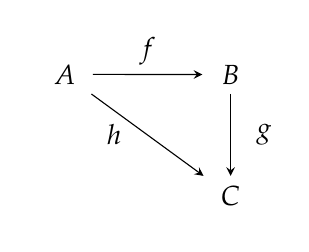
\begin{tikzpicture}
		\matrix (m) [matrix of math nodes,row sep=3em,column sep=4em,minimum width=2em]
		{
			A & B  \\ 
			& C\\};
		\path[-stealth]
		(m-1-1) edge node [above] {$f$} (m-1-2)
		(m-1-1) edge node [left]  {$h~~$} (m-2-2)
		(m-1-2) edge node [right] {$~~g$} (m-2-2);
	\end{tikzpicture}
	\\ 	
	It will be said to \textit{commute} if $h = g\circ f$. The point is that the diagram offers 
	two paths from $A$ to $C$, either by composing to follow $f$ and then $g$, or by 
	following h directly. Commutativity means that the two paths amount to 
	the same thing. A more complex diagram, like the previous one, is said to 
	be commutative when all possible triangles that are parts of the diagram 
	are themselves commutative. This means that any two paths of arrows in 
	the diagram that start at the same object and end at the same object 
	compose to give the same overall arrow. By a \textit{diagram} $D$ in a 
	category $\mathscr C$ we simply mean a collection of $\mathscr C$-objects $d_j, d_k,...$ together 
	with some $\mathscr C$-arrows $g: d_j \to d_k$ between certain of the objects in the 
	diagram. (Possibly more than one arrow between a given pair of objects, 
	possibly none). 
	A \textit{cone} for diagram $D$ consists of a $\mathscr C$-object $c$ together with a $\mathscr C$-arrow 
	$c\to d_j$ for each object $f_j$ in $D$, such that
	\newline
	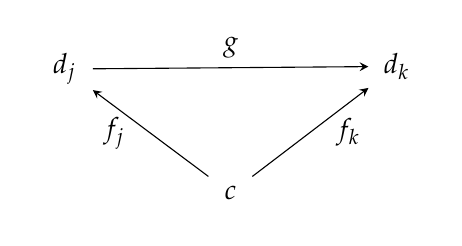
\begin{tikzpicture}
		\matrix (m) [matrix of math nodes,row sep=3em,column sep=4em,minimum width=2em]
		{
			d_j  & & d_k \\ 
			& c  & \\};
		\path[-stealth]
		(m-1-1) edge node [above] {$g$} (m-1-3)
		(m-2-2) edge node [left]  {$f_j~~$} (m-1-1)
		(m-2-2) edge node [right] {$~~f_k$} (m-1-3);
	\end{tikzpicture}
	\\ 	
	commutes, whenever g is an arrow in the diagram $D$. We use the 
	symbolism $\left\{f_j: c\to d_j\right\}$ to denote a cone for $D$. 
	
	
	A \textit{limit} for a diagram $D$ is a $D$-cone $\left\{f_j: c\to d_j\right\}$ with the property that for 
	any other $D$-cone $\left\{f'_j: c'\to d_j\right\}$ there is exactly one arrow $f:c' \to c$ such 
	\newline
	\begin{tikzpicture}
		\matrix (m) [matrix of math nodes,row sep=3em,column sep=4em,minimum width=2em]
		{
			& d_j &  \\ 
			c'	&  & c \\};
		\path[-stealth]
		(m-2-1) edge node [above] {$g$} (m-2-3)
		(m-2-1) edge node [left]  {$f'_j~~$} (m-1-2)
		(m-2-3) edge node [right] {$~~f_j$} (m-1-2);
	\end{tikzpicture}
	\\ 	
	commutes for every object $d_j$ in $D$. 
	This limiting cone, when it exists, is said to have the \textit{universal property} 
	with respect to $D$ -cones.
	A limit for 
	diagram $D$ is unique up to isomorphism.%:- if {ft: �> a\} and {f-:c'�> d;} 			are both limits for D, then the unique commuting arrow f: c'� above is 			iso (its inverse is the unique commuting arrow c-�*c' whose existence 			follows from the fact that {/,': c' �> dj is a limit). 
			% It is universal amongst such cones-any other 		D-cone factors uniquely through it as in the last diagram.		
			
			
			\begin{definition}\label{pull_back_defn}\cite{goldblatt:topoi}
				A \textit{pullback} of a pair $a \xrightarrow{f}c \xleftarrow{g} b$ of $\mathscr C$-arrows with a common codomain 
				is a limit in $\mathscr C$ for the diagram 
				\newline
				\begin{tikzpicture}
					\matrix (m) [matrix of math nodes,row sep=3em,column sep=4em,minimum width=2em]
					{
						& b  \\ 
						a	&  c \\};
					\path[-stealth]
					(m-1-2) edge node [right]  {$g$} (m-2-2)
					(m-2-1) edge node [above] {$f$} (m-2-2);
				\end{tikzpicture}
				\\ 	
				
			\end{definition}
			
				\begin{definition}\label{pullback_defn}\cite{milne:lec}
				For $X$ an object of a category $\mathscr C$, $\mathscr C/X$ denotes the category whose objects are the morphisms $U\to X$ in $\mathscr C$
				and whose arrows are the commutative diagrams 
				\newline
				\begin{tikzcd}
					U \arrow[rr]\arrow[rd] && U'\arrow[ld]\\
					& X &
				\end{tikzcd}
				\\
				A morphism $U \to U'$ making this diagram commute is also referred to as an $X$-\textit{morphism}. The \textit{fibre product} or the \textit{pullback} $U_1\times_X U_2$ of morphisms $\varphi_1: U_1\to X$,  $\varphi_2: U_2\to X$ in $\mathscr C$ is their product in the category $\mathscr C/X$. Thus, there is a commutative diagram 
				\newline
				\begin{tikzcd}
					U_1\times_X U_2 \arrow[d] \arrow[r]
					& U_2 \arrow[d, "\varphi_2"]\\
					U_1\arrow[r, "\varphi_1"]	& X
				\end{tikzcd}
				\\
				\\
				having the obvious universal property. 
				
			\end{definition}
			
			\begin{defn}\label{sets_cat_defn}\cite{johnstone:topos}
				There is the \textit{category  of sets and functions} $\mathscr{S}$. We use the therm \textit{small category} for a category those morphisms form a set. If $\mathscr C$ is a small category, we write $\mathscr{S}^{\mathscr{C}^{\mathrm{op}}}$ for the category of \textit{presheaves}, i.e. contravariant functors from $\mathscr{C}$ to $\mathscr{S}$; among the objects of $\mathscr{S}^{\mathscr{C}^{\mathrm{op}}}$, we have the \textit{representable} functors $h_U$, where $U$ is an object of $\mathscr C$, defined by $h_U\left( V\right) \bydef \Hom_{\mathscr{C}}\left( V, U\right)$; we shall also write $h^U$ for the covariant representable  functor $\Hom_{\mathscr{C}}\left( U, -\right)$.
			\end{defn}
			\begin{lemma}\label{repr_func_lem}\cite{johnstone:topos}
				For objects $U$, $X$ of $\mathscr{C}$ and $\mathscr{S}^{\mathscr{C}^{\mathrm{op}}}$ respectively there is a bijection (natural in both variables) between morphisms $h_U \to X$ in $\mathscr{S}^{\mathscr{C}^{\mathrm{op}}}$ and elements of the set $X\left(U \right)$. 
			\end{lemma}
			\begin{lemma}\label{to_set_lem}\cite{johnstone:topos}
				Any object of $\mathscr{S}^{\mathscr{C}^{\mathrm{op}}}$ can be expressed as a colimit of a diagram whose vertices are representable functors.
			\end{lemma}
			
\begin{definition}
	\label{(co)complete_defn}A category $\mathbf{C}$ is called \textit{complete}
	if it admits small limits, and \textbf{cocomplete} if it admits small
	colimits.
\end{definition}
			
\subsection{Functors}
\begin{definition}\label{functor_defn}\cite{goldblatt:topoi}
	A \textit{functor} $F$ from category $\mathscr{C}$ to category $\mathscr{D}$ is a function that assigns 
	\begin{enumerate}
		\item [(i)]
		to each $\mathscr{C}$-object $a$, a $\mathscr{D}$-object $F(a)$; 
		\item[(ii)] to each $\mathscr{C}$-arrow $f:a \to b$ a $\mathscr{D}$-arrow $F(f): F(a) \to F(b)$, 
		such that 
		\begin{enumerate}
			\item[(a)]  $F\left(\mathbb 1_a\right) = \mathbb 1_{F\left(a\right)}$ for all  $\mathscr{C}$-objects $a$, i.e. the identity arrow on $a$ is assigned 
			the identity on $F\left(a\right)$,
			\item[(b)]  $F\left(g\circ f\right)=F\left(g\right)\circ F\left( f\right) $, whenever $g \circ f$ is defined. 
			This last condition states that the $F$-image of a composite of two arrows 
			is the composite of their $F$-images.
		\end{enumerate}
		
		
	\end{enumerate}
	We write $F:\mathscr{C}\to \mathscr{D}$ or  $\mathscr{C}\xrightarrow{F} \mathscr{D}$ to indicate that $F$ is a 
	functor from $
	\mathscr{C}$ to $\mathscr{D}$. Briefly then a functor is a transformation that 
	"preserves" dom's, cod's, identities and composites. 
\end{definition}
If $a$ and $b$ are  $\mathscr{C}$-objects then a functor $\mathscr{C}\xrightarrow{F} \mathscr{D}$ yields a map
\be\label{f_ab_funct_eqn}
F_{a,b}:\mathscr{C}\left(a, b \right)  \to \mathscr{D}\left( F\left(a\right), F\left(b\right)\right)  
\ee
(cf. Notation \ref{category_not}).
\begin{definition}\label{funct_full_faithfull_defn}\cite{bass}
	A functor $\mathscr{C}\xrightarrow{F} \mathscr{D}$ is said to be \textit{faithful} (resp. \textit{full}) if the given by \eqref{f_ab_funct_eqn} map is injective (resp. surjective).
\end{definition}
\begin{defn}\label{functor_contravariant_defn}\cite{goldblatt:topoi}
	A \textit{contravariant} functor is one that reverses direction by mapping domains 
	to codomains and vice versa. 
	Thus $\mathscr{C}\xrightarrow{F} \mathscr{D}$ is a contravariant functor if it assigns to $f: a\to b$ an 
	arrow $F(f):F(b)\to F(a)$, so that $F\left(\mathbb{1}_a\right)= \mathbb{1}_{F(a)}$ as before, but now 
	$$
	F\left( g\circ f\right) = F\left( f\right)\circ  F\left( g\right). 
	$$
\end{defn}


\begin{definition}\label{exact_functor_defn}\cite{goldblatt:topoi}
	A left/right exact functor is a functor that preserves finite limits/finite colimits.
\end{definition}
\subsection{Natural transformations}\label{natural_transformation_sec}
\paragraph{}
Here I follow to \cite{goldblatt:topoi}.
Given two categories $\mathscr C$ and $\mathscr D$ we are going to construct a category, 
denoted $\mathrm{Funct}\left(\mathscr C, \mathscr D\right)$, or $\mathscr D^{\mathscr C}$, whose objects are the functors from $\mathscr C$ to $\mathscr D$. 
We need a definition of arrow from one functor to another. Let 
$F: \mathscr C\to \mathscr D$ and $G: \mathscr C\to \mathscr D$ be two functors. For any $\mathscr C$-object $a$ we define a $\mathscr D$-arrow $\tau_a : F\left(a\right)\to  G\left(a\right)$. We require that each  $\mathscr C$-arrow $f: a \to b$  gives rise to a diagram 
\\
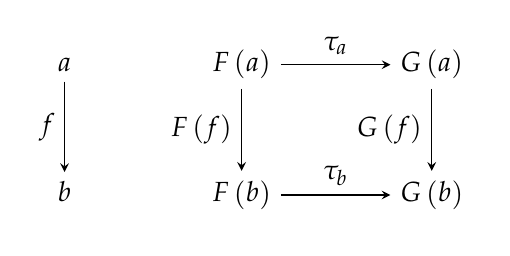
\begin{tikzpicture}
	\matrix (m) [matrix of math nodes,row sep=3em,column sep=4em,minimum width=2em]
	{
		a	& F\left(a \right)  &   G\left(a \right)\\ 
		b	& F\left(b \right)  &   G\left(b \right) \\};
	\path[-stealth]
	(m-1-1) edge node [left]  {$f$} (m-2-1)
	(m-1-2) edge node [above] {$\tau_a$} (m-1-3)
	(m-2-2) edge node [above]  {$\tau_b$} (m-2-3)
	(m-1-2) edge node [left]  {$F\left( f \right)$} (m-2-2)
	(m-1-3) edge node [left]  {$G\left( f \right)$} (m-2-3);
\end{tikzpicture}
\\ 	
that commutes.
%a F(a) Ta > G(a) Ftf)  F(b) T"  G(b) that commutes. Thus  and provide a categorical way of turning the F-picture of f:a-*b into its G-picture. 
In summary then, a \textit{natural transformation} from functor $F: \mathscr C\to \mathscr D$ and $G: \mathscr C\to \mathscr D$  to functor $F: \mathscr C\to \mathscr D$ and $G: \mathscr C\to \mathscr D$  is an assignment $\tau$ that provides, for each $\mathscr C$-object $\mathscr D$-arrow $\tau_a :F(a) \to G(a)$, such that for any $\mathscr C$-arrow $f:a\to b$, the above diagram commutes in $\mathscr D$, i.e. $\tau_b \circ F(f)= G(f)\circ \tau_a$. We use the symbolism $\tau: F\to G$, or $F \xrightarrow{\tau}G$, to denote that $\tau$ is a natural transformation from $F$ to $G$. The arrows $\tau_a$ are called the \textit{components} of $a$. Now if each component $\tau_a$ of $a$ is an iso arrow in $\mathscr D$ then  case we call $\tau$ a \textit{natural isomorphism}. Each $\tau_a: F(a)\to G(a)$ then has an inverse $\tau_a^{-1}: G(a) \to F(a)$, and these $\tau^{-1}_a$'s form the components of a natural isomorphism $\tau^{-1}: G \to F$. We denote natural isomorphism by $\tau: F \cong G$. 
\begin{example}
	The identity natural transformation $\mathbb{1}_F :F\to F$ assigns to each object $a$, the identity arrow $\mathbb{1}_{F(a)}:F(a)\to F(a)$. This is clearly a natural isomorphism. 
\end{example}

\begin{definition}\label{category_equivalence_definition}\cite{goldblatt:topoi}
	A functor $F: \mathscr C\to  \mathscr D$ is called an \textit{equivalence of categories} if there 
	is a functor $G: \mathscr D\to  \mathscr C$ such that there are natural isomorphisms $\tau : 1_{\mathscr C} \cong G \circ F$, and $\sigma : 1_{\mathscr D} \cong F \circ G$, from the identity functor on ${\mathscr C}$ to $ G \circ F$, and 
	from the identity functor on ${\mathscr D}$ to $ F \circ G$.
	
	Categories $\mathscr C$ and $\mathscr D$ are \textit{equivalent},  $\mathscr C$ and $\mathscr D$ when there exists an equivalence $F: \mathscr C\to  \mathscr D$ .
\end{definition}

			



%We assume that reader is familiar with the notions of \textit{limit} and \text{colimit}.


\subsection{Adjoint functors}\label{adjoint_functor_sec}
\paragraph*{}

If both $\mathscr C$ and $\mathscr D$ are categories then a pair of functors $\mathscr C \substack{ \xrightarrow{F}\\\xleftarrow[G]{}}\mathscr D$ are \textit{adjoint functors} if for any $\mathscr C$-object $A$ and $\mathscr D$-object $B$ there is a natural bijection
$$
\Hom_{\mathscr D}\left(F\left(A \right), B  \right) \cong \Hom_{\mathscr C}\left(A, G\left(B \right)  \right).
$$
	A pair of {adjoint functors} can be defined via counit�unit adjunction, i.e. there are natural transformations
\bean
\eps : FG \to 1_{\mathscr C},\\
\eta : 1_{\mathscr  D} \to  GF 
\eean
respectively called the \textit{counit} and the \textit{unit} of the adjunction (terminology from universal algebra), such that the compositions
		\be\label{id_thens_eqn}
		\begin{split}
F{\xrightarrow {\;F\eta \;}}FGF{\xrightarrow {\;\varepsilon F\,}}F,\\
G{\xrightarrow {\;\eta G\;}}GFG{\xrightarrow {\;G\varepsilon \,}}G
		\end{split}
\ee
are the identity transformations $1_F$ and $1_G$ on $F$ and $G$ respectively. $F$ is said to be \textit{left adjoint} $G$, and $G$ is \textit{right adjoint} $F$.
\section{Elementary topoi}

\begin{definition}\label{topos_defn}\cite{johnstone:topos}
A category $\mathcal E$ is called an (elementary) \textit{topos} if
\begin{enumerate}
	\item [(a)]  $\mathcal E$ has all finite limits (Equivalently,  $\mathcal E$ has pullbacks and a terminal object).
	\item[(b)]  $\mathcal E$ is \textit{cartesian closed}, i.e. for each object $X$ we have an \textit{exponential functor} $\left(-\right)^X$ which is right adjoint to the functor $\left(-\right)\times X$.
	\item[(c)] $\mathcal E$ has a \textit{subobject classifier}, i.e. an object $\Om$ and a morphism $1 \xrightarrow{t} \Om$ (called "true") such that for each monomorphism $Y \xhookrightarrow{\sigma} X$ there is a unique $\phi_\sigma: X \to \Om$ (the \textit{classifying map} of $\sigma$) making 
		\newline
	\begin{tikzcd}
		Y \arrow[d, hook, "\sigma"] \arrow[r]
		& 1 \arrow[d, "t"]\\
	X\arrow[r, "\phi_\sigma"]	& \Om
	\end{tikzcd}
	\\
	a pullback diagram.
\end{enumerate}
\end{definition}
\begin{example}\label{sets_exm}\cite{johnstone:topos}
A category category  of sets and functions $\mathscr S$ (cf. Definition \ref{sets_cat_defn}) of sets is a topos.
\end{example}
	\begin{definition}\label{geometric_morphism_defn}\cite{johnstone:topos}
	% 1.16 
	If both $\mathscr E$, $\mathscr F$ are toposes then \textit{geometric morphism} $\mathscr F\xrightarrow{f}\mathscr E$ consists of a pair of functors $\mathscr F\xrightarrow{f_*}\mathscr E$  and $\mathscr E\xrightarrow{f^*}\mathscr F$ (called the \textit{direct} and \textit{inverse images}) such that $f^*$ is left adjoint to $f_*$ and $f^*$ is left exact. 
\end{definition}
%\begin{definition}\label{relative_topos_defn}\cite{johnstone:topos}
%For any topos $\mathscr E$ there is a category $\mathfrak {Top}/\mathscr E$. Objects of  $\mathfrak {Top}/\mathscr E$ are $\mathscr E$-\textit{toposes}, i.e. toposes $\mathscr F$ with geometric $\mathfrak {Top}/\mathscr E$-morphisms $\mathscr F\to \mathscr E$, morphisms are commutative diagrams
%		\newline
%\begin{tikzcd}
%\mathscr F' \arrow[rr]\arrow[rd] && \mathscr F''\arrow[ld]\\
%& \mathscr E &
%\end{tikzcd}
%\\

%\end{definition}




	\section{Grothendieck topology, sheaves and cosheaves}
	
	\subsection{Sites}\label{appendix_etale_sec}

	\begin{definition}\label{pretopology_defn}\cite{johnstone:topos,milne:lec}
		Let  $\mathscr C$  be a category with pullbacks. Suppose that  for each object $U$ of $\mathscr C$ there are  distinguished sets of families of morphisms $\left\{U_\iota \to U\right\}_{\iota\in I}$, called the \textit{coverings} of $U$, 
		satisfying the following axioms: 
		\begin{enumerate}
			\item[(a)] for any covering $\left\{U_\iota \to U\right\}_{\iota\in I}$ and any morphism $U \to V$ in $\mathscr C$, the fibre products 
			$U_\iota\times_U V$ exist, and $\left\{U_\iota\times_U V \to V\right\}_{\iota\in I}$ is a covering of $V$; 
			\item[(b)] if $\left\{U_\iota \to U \right\}_{\iota\in I}$ is a covering of $U$, and if for each $\iota \in I$, $\left\{V_{\iota j} \to U_\iota  \right\}_{j \in I_\iota}$	is a 
			covering of $U_\iota$, then the family $\left\{V_{\iota j }\to U\right\}_{\iota j}$ is a covering of $U$; 
			\item[(c)] for any $U$ in $\mathscr C$, the family $\left\{U\xrightarrow{\Id}U \right\}$ consisting of a single map is a covering of $U$. 
		\end{enumerate}
		The system of coverings is then called a \textit{Grothendieck pretopology}.
	\end{definition}
	\begin{example}\label{top_gro_exm}
		If $\sX$ is a topological space then one has a category of open subsets and their inclusions. If both $\sU_1, \sU_2 \subset \sX$ are open subsets then one can define a fibre product (cf. Definition \ref{pullback_defn}) by the following way
		$$
		\sU_1\times_\sX \sU_2 \bydef \sU_1 \cap \sU_2.	
		$$
		If $\sU \subset \sX$ is an open subset then we assume that a family  $\left\{\sU_\iota \subset \sU\right\}_{\iota\in I}$, is a covering of $\sU$ (cf. Definition \ref{pretopology_defn}) if and only if  $\sU = \cup_{\iota\in I}\sU_\iota$. This system of coverings is a specialization of Grothendieck pretopology. 
	\end{example}
	\begin{definition}\label{top_gro_definition}
		In the situation of the Example \ref{top_gro_exm} one has a site $\mathbf T_{\sX}$ \textit{arising} from $\sX$.
	\end{definition}
	\subsection{Sheaves and cosheaves}
	\begin{definition}\label{etale_presheaf_defn}\cite{milne:lec}
		A \textit{presheaf of sets} on a category $\mathscr C$
		is a contravariant functor $\mathscr F$ from $\mathscr C$ to the category of sets. Thus,  $\mathscr F$
		to each object $U$ in $\mathscr C$ 
		attaches a set $\mathscr F\left(U \right)$ , and to each morphism $\varphi: U \to V$
		in $\mathscr C$, a map $\mathscr F\left(\varphi\right):\mathscr F\left(V \right)\to \mathscr F\left(U \right)$. Note that the notion of a presheaf on $\mathscr C$ 
		does not depend on the 
		coverings. We sometimes denote $\mathscr F\left(\varphi\right)$ by $a \mapsto a|_U$.
		
	\end{definition}
	\begin{remark}\label{etale_presheaf_rem}\cite{milne:lec}
	Similarly, a presheaf of (Abelian) groups or rings for the Grothendieck pretopology is a contravariant functor from
$\mathscr C$ to the category of (Abelian) groups or rings.
	\end{remark}
	\begin{definition}\label{etale_sheaf_defn}\cite{milne:lec}
		A \textit{sheaf} for the Grothendieck pretopology
		is a presheaf $\mathscr F$ 
		that satisfies the sheaf condition, that is a sequence 
		\be\label{sheaf_eqn}
		\mathscr F \left(U\right) \to \prod_{\iota \in I} \mathscr F \left(U_\iota \right)\rightrightarrows  \prod_{\iota, j \in I\times I} \mathscr F \left(U_\iota \times_U U_j\right)
		\ee
		is exact for every covering $\left\{U_\iota \to U\right\}$. Thus $\mathscr F$ 
		is a sheaf if the map 
		$$
		f \mapsto \left\{f|_{U_\iota }\right\}:\mathscr F \left(U\right) \to \prod_{\iota \in I} \mathscr F \left(U_\iota \right)
		$$
		identifies $\mathscr F\left( U\right)$ with the subset of the product consisting of families $\left\{f|_{U_\iota }\right\}$ such that 
		$$
		f_\iota|_{U_\iota \times_U U_j}= f_j|_{U_\iota \times_U U_j}
		$$
		for all $\iota, j \in I$. 
		When $\mathbf T$ 
		is the site arising from a topological space then these definitions coincide with the 
		topological ones. 
		
	\end{definition}
	\begin{empt}\cite{johnstone:topos}
	Two different Grothendieck pretopologies can give the same sheaves. To remove this disadvantage we consider those families which are "saturated" in the sense that $\left(V \xrightarrow{\a}U\right) \in R$ implies $\left(W\xrightarrow{\a\bt}U\right)\in \R$ for any $W \xrightarrow{\bt} V$. Such a family is called a \textit{sieve}.
	\end{empt}
	\begin{defn}\label{grotendieck_topolgy_defn}\cite{johnstone:topos}
		Let $\mathscr C$ be a small category. A \textit{Grothendieck topology} on $\mathscr C$ is defined by specifying, for each object $U$ of $\mathscr C$ a set $J\left(U\right)$ of {sieves} called \textit{covering sieves} of the topology such that
		\begin{enumerate}
			\item [(a)] For any $U$, the maximal sieve $\left\{\a | \text{codomain}(a)= U\right\}$ is in $J\left(U \right)$.
			\item[(b)] if $R \in J\left( U\right)$ and $V\xrightarrow{f} U$ is a morphism of $\mathscr C$ then the sieve
			$$
			f^*\left( R\right) \bydef \left\{W\xrightarrow{a}V| f\a \in R \right\}
			$$
			is in $J\left(V\right)$.
			\item[(c)] If $R \in J\left(U \right)$ is sieve on $U$ such that for each $V\xrightarrow{f}U$ in $R$ we have $f^*\left( S\right)\in J\left( V\right)$, then $S\in J\left( U\right)$.    
			
		\end{enumerate}
A category $\mathscr C$  together with 
		the Grothendieck  topology is called a \textit{site} $\mathbf T\bydef \left( \mathscr C, J\right)$. Then $\mathrm{Cat}\left( \mathbf T\right)\bydef \mathscr C$ denotes the underlying category. 
		
\end{defn}
\begin{rem}\label{pretopology_to_topology_rem}\cite{johnstone:topos}
If we are given a pretopology $P$ on  $\mathscr C$, we can replace it be a topology having same sheaves, by defining a sieve to be $J$-covering if and only if it contains $P$-covering family.
\end{rem}
	\begin{definition}\label{forget_sheaf_defn}
		There are categories $\mathbf{PreSh}\left(\mathbf T \right)$, $ \mathbf{Sh}\left(\mathbf T\right)$ of presheaves an sheaves. Moreover there is a \textit{forgetful functor} $\mathfrak{Forget} : \mathbf{Sh}\left(\mathbf T \right)\to \mathbf{PreSh}\left(\mathbf T \right)$.
	\end{definition}
	
	\begin{statement}\label{associated_sheaf_stmnt}\cite{johnstone:topos}
		There is an adjoint $\mathfrak{Ass} : \mathbf{PreSh}\left(\mathbf T  \right)\to \mathbf{Sh}\left(\mathbf T \right)$ to the  forgetful functor $\mathfrak{Forget} : \mathbf{Sh}\left(\mathbf T  \right)\to \mathbf{PreSh}\left(\mathbf T \right)$ (cf. Definition \ref{forget_sheaf_defn}).
	\end{statement}	
	\begin{defn}\label{associated_sheaf_defn}\cite{johnstone:topos}
		The given by the Statement  \ref{associated_sheaf_stmnt} functor $\mathfrak{Ass} : \mathbf{PreSh}\left(\mathbf T  \right)\to \mathbf{Sh}\left(\mathbf T \right)$  is said to be an  \textit{associated sheaf functor}.
	\end{defn}
		\begin{rem}\label{ab_uss_rem}
		Similarly there are categories re categories $\mathbf{PreShAb}\left(\mathbf T \right)$, $ ~~\mathbf{Ab}\left(\mathbf T\right)$ of presheaves an sheaves of Abelian groups (cf. Remark \ref{etale_presheaf_rem}). Also there a functors $\mathfrak{Forget} : \mathbf{Ab}\left(\mathbf T \right)\to \mathbf{PreShAb}\left(\mathbf T \right)$ and $\mathfrak{Ass} : \mathbf{PreShAb}\left(\mathbf T  \right)\to \mathbf{Ab}\left(\mathbf T \right)$. The functor $\mathfrak{Ass}$ is an adjoint to $\mathfrak{Forget}$.
	\end{rem}
	
	\begin{statement}\label{site_enough_stmt}\cite{johnstone:topos}
		%8.13$
		If $\mathbf T$ is a site then a category $\mathbf{Ab}\left(\mathbf T \right)$ of sheaves of Abelian groups has enough injectives.
	\end{statement}
	\begin{definition}\label{grothenidieck_topos_defn}\cite{johnstone:topos}
		If $\mathbf T$ is a site then  a category  $\mathbf{Sh}\left( \mathbf T \right)$ of sheaves of sets is a \textit{Grothendieck topos}.
	\end{definition}
		\begin{definition}\label{grothendiek_topos_defn}\cite{johnstone:topos}
		A category $\mathscr E$ is said to be a \textit{Grothendieck topos} if there exist a site $\mathbf T$ such that $\mathscr E$ is equivalent to a category  $\mathbf{Sh}\left(\mathbf T  \right)$ of sheaves of sets on $\mathbf T$.
	\end{definition}
	
	
	\begin{proposition}\label{grothenidieck_topos_prop}\cite{johnstone:topos}
Any {Grothendieck topos} is a topos in the sense of the Definition \ref{topos_defn}.
\end{proposition}
%\begin{remark}\cite{johnstone:topos}
%If $\mathscr E$ is  a {Grothendieck topos} and $\mathscr S$ is a category of sets and functions then $\mathscr E$ is $\mathscr S$-topos (cf. Definition \ref{relative_topos_defn}).
%\end{remark}

	%\begin{rem}\label{geom_mor_g_rem}\cite{johnstone:topos}
	% 1.16 Grothendieck
	%If both $\mathscr E$, $\mathscr F$ are Grothendieck toposes and  $\mathscr F\xrightarrow{f}\mathscr E$ is {geometric morphism} then direct image $f^*$ is left exact. 
	%\end{rem}
	\begin{definition}\label{constant_presheaf_defn}\cite{johnstone:topos}
		If $X$ is an object of $\mathrm{Cat}\left( \mathbf T\right)$ (cf. Definition \ref{pretopology_defn}    then for any set $F$ there is a \textit{constant presheaf} $\mathscr P$ such that $\mathscr P\left( U\right) \bydef F$ and $\mathscr P\left( f\right) \bydef \Id_F$ for all $\mathrm{Cat}\left( \mathbf T\right)/X$-morphism $f: U\to V$.
		We use a following notation
		\be\label{constant_presheaf_eqn}
		F_X \bydef \mathscr P.
		\ee
	\end{definition}

\paragraph{}

\begin{definition}\label{coheaf_defn}\cite{shimizu_cosh}
Let $X$ be a small category equipped with a pretopology $J$ and $\V$ be a category. 
Recall that a functor $\mathscr G : X \to \V$ is called a \textit{precosheaf} on $X$. 
It is called a \textit{cosheaf} if the diagram
\begin{equation}\label{coeq cosh}
	\coprod_{j,k \in I} \mathscr G(U_j \times_U U_k) \rightrightarrows \coprod_{i \in I} \mathscr G(U_i) \to \mathscr G(U)
\end{equation}
is a coequalizer in $\V$ for all $\{U_i \to U\}_i \in J$. 
In other words, a cosheaf is a $\V^{\mathrm{op}}$-valued sheaf. If $X$ is a site or a locale then we denote by $\mathbf{PreCSh}\left(X \right)$ and  $\mathbf{CSh}\left(X \right)$ a category of precosheafs and cosheaves respectively.
\end{definition}




		\subsection{Localic topoi}
	\begin{definition}\label{frame_defn}\cite{topos:intro}
A \textit{frame} is lattice with all joins and all finite meets which satisfies the infinite distributive law:
\be\label{frame_eqn}
x \wedge \left( \bigvee_\iota y_\iota \right) = \bigvee_\iota\left(x\wedge   y_\iota \right) 
\ee
A \textit{frame homomorphism} 
is a function which preserves finite meets and arbitrary joins. Notice
that any frame has a largest element 1 (the empty meet) and a smallest
element 0 (the empty join); thus a morphism   of frames $\Phi: B \to A$
satisfies
\be\label{locale_mor_eqn}
\begin{split}
\Phi\left(0\right)= 0,\\
\Phi\left(1\right)= 1,\\
\Phi\left(U\wedge V\right) = \Phi\left(U\right)\wedge  \Phi\left(V\right),\\
\Phi\left(\bigvee U_\iota\right) = \bigvee \Phi\left(U_\iota\right).\\
\end{split}
\ee

for all elements $U_\iota$ , $U$, and $V$ of $B$.

 Frames and frame homomorphisms form a category $\mathbf{Frm}$.
	\end{definition}
		\begin{definition}\label{locale_defn}\cite{topos:intro}
		The category $\mathbf{ Locale}$ of \textit{locales} is the opposite of the category of frames
		$$
		\mathbf{ Locale} \bydef \mathbf{Frm}^\text{op}.
		$$
		If $X$ is  a locale  denote by $\mathcal O\left( X\right)$ the corresponding  frame.
	\end{definition}
	The definition  of sheaves on a topological space depends
	only on the lattice of open sets of that space, and so extends at once to
	define sheaves on a locale $X$. Thus an "open" object $U$ is underlying category is said to be
	covered by a family $\left\{U_\iota \right\}$ of "opens" of $X$ with each $U_\iota \le U$  if and only if $U= \bigvee_\iota V_\iota$ thus
	\be\label{localic_site}
	\left\{U_\iota\subset U \right\} \text{ covers } U \text{ if and only if } U= \bigvee_\iota V_\iota
	\ee
	The equation \eqref{localic_site} yields a Grothendieck pretopology, so one obtains a Grothendieck topology. In result we obtain a site and a Grothendieck topos.
	
\begin{definition}\label{localic_topos_defn}\cite{topos:intro}
	A Grothendieck topos obtained from a locale is said to be \textit{localic}.
\end{definition}
	\begin{theorem}\label{locale_thm}\cite{topos:intro}
		For a Grothendieck $\mathscr E$ the following are equivalent:
		\begin{enumerate}
			\item [(i)] $\mathscr E$ is localic,
			\item[(ii)] there exists a site for $\mathscr E$ with a patrially ordered set as underlying category,
			\item[(iii)] $\mathcal{E}$ is generated by the subobjects of its terminal object 1.
		\end{enumerate}
	\end{theorem}
	

\begin{proposition}\label{locale_funct_prop}\cite{topos:intro}
%Proposition 2. 
The natural  functor $X \mapsto \mathbf{ Sh}(X)$ from locales to topoi induces
for any two locales $X$ and $Y$ an equivalence of categories
$$
\mathbf{Maps}(X, Y) \xrightarrow{\cong} \Hom\left( \mathbf{Sh}(X), \mathbf{Sh}(Y)\right) 
$$
of locales and localic toposes.

\end{proposition}


\subsection{Spatial locales}\label{spatial_toposes_sec}
\paragraph*{}	
Any topological space $\sX$ yields a Grothendieck topology, so 	a Grothendieck topology is a generalization of the classical topology. A topos is \textit{spatial} if it corresponds to a classical topology.
%\begin{definition}\label{topos_point_defn}\cite{johnstone:topos}
%Let $\mathscr S$ be a category of sets and functions, and let $\mathscr E \xrightarrow{\ga} \mathscr S$ be an $\mathscr S$-topos (cf. Definition \ref{relative_topos_defn}). By a \text{point} of $\mathscr E$ we mean a Geometric morphism $\mathscr S \xrightarrow{p} \mathcal E$ over $\mathscr S$. If $K$ is a class of points, we say that $K$ is \textit{sufficient} if the family of functors $\left\{\left.p^*\right| p\in K\right\}$ is conservative, i.e. if any $X \xrightarrow{f} Y$ in $\mathscr E$ such that $p^*\left(f \right)$ is iso for all $K$ is necessary iso. We say that $\mathscr E$ \text{has enough points} if the class of all points of $\mathscr E$ is sufficient.
%\end{definition}
%\begin{example}\label{top_points_exm}\cite{johnstone:topos}
%Let  $\mathcal E \bydef \mathbf{Sh}\left( \sX\right)$,  $\sX$ is a topological space. Then any point $x$ of $\sX$ corresponds to a continuous map ${x} \xrightarrow{x}\sX$. Moreover, the set of points which arise in this way is sufficient.
%\end{example}


\begin{definition}\label{locale_point_defn}\cite{topos:intro}
A	\textit{point} $p: 1\to X$ of a locale $X$ is the same thing
	as a frame morphism to the initial frame
	\be\label{locale_point_eqn}
	p^{-1}:\mathcal{O}\left( X \right) \to \left\{0, 1\right\}.
	\ee
\end{definition}
	The map $p^{-1}$ can be conveniently presented in terms of its \textit{kernel} $K \bydef
\left\{U \left.| p^{-1} \left( U \right)  = 0\right.\right\}$, a subset of $X$ with the following properties
\be\label{k_p_eqn}
\begin{split}
1 \notin K,\\
U \wedge V \in K\quad  \Leftrightarrow \quad U \in K \text{ or } V \in K,\\
\bigvee V_\iota \in K \quad  \Leftrightarrow \quad \forall \iota \quad V_\iota \in K
\end{split}
\ee
If
\be\label{p_p_eqn}
 P \bydef  \bigvee K \bydef \left( \bigvee_{U\in K} U\right) \in \mathcal O\left( X\right) 
 \ee
 then
 \bea\label{prime_eqn}
U\wedge V = P  \quad  \Leftrightarrow \quad U \le P \text{ or } V\le P,\\
\label{pprime_eqn}
1 \neq P.
 \eea
 A satisfying to \eqref{prime_eqn} element $P\in \mathcal O\left(X \right)$ is said to be \textit{prime}, if it also satisfies to  \eqref{pprime_eqn} then we say that $P$ is. \textit{properly prime}.
\begin{lemma}\label{point_lem}\cite{topos:intro}
The points of a locale $X$ may be described in any of the
following three equivalent ways:
\begin{enumerate}
	\item[(i)] as maps of locales $p: 1 \to X$; i.e., as frame morphisms
		$p^{-1}:\mathcal{O}\left( X \right) \to \left\{0, 1\right\}$;
	\item[(ii)] as subsets $K \subset \mathcal{O}\left( X \right)$ satisfying the three conditions of \eqref{k_p_eqn};
	\item[(iii)] as proper prime elements $P \in  \mathcal{O}\left( X \right)$); i.e., as elements $P\in \mathcal{O}\left( X \right)$ satisfying \eqref{prime_eqn} and \eqref{pprime_eqn}.
\end{enumerate}
\end{lemma}

This set of points carries a natural
topology for which the open sets are the sets of the form
\be\label{point_set_eqn}
\mathrm{pt}(U) = \left\lbrace p \in \mathrm{pt}(X) \left| p^{-1}\left( U\right)  = 1\right.\right\rbrace \subset \mathrm{pt}(X)\quad \text{ for some }\quad U \in \mathcal O\left(X\right)
\ee
From a map $f: X\to Y$ of locales one can construct a continuous map $\mathrm{pt}(X)\to \mathrm{pt}(Y)$ of topological spaces, i.e.
\be\label{sober_map}
\mathrm{pt}(f): (p: 1 \to X) \mapsto  (f \circ p : 1 \to X \to Y). 
\ee
Thus there is a functor 
\be\label{point_f_eqn}
\mathrm{pt}: \mathbf{Locales}\to \mathbf{Spaces}
\ee
from the category of locales to the category of topological spaces (cf. \cite{topos:intro} for details).
\begin{theorem}
The functor $\mathrm{pt}: \mathbf{Locales}\to \mathbf{Spaces}$ is right adjoint
to the functor $\mathrm{Loc} : \mathbf{Spaces} \to \mathbf{Locales}$.
\end{theorem}


\begin{definition}\label{sober_defn}\cite{topos:intro}
A topological space $\sX$ is said to be \textit{sober} if and only is for any
open subset $\sU\subset \sX$ such that
\begin{enumerate}
	\item[(a)] $\sU \neq \sX$,
	\item[(b)] $\sV \cap \mathcal W \subset \sU \Rightarrow \sV \subset \sU$ or $\mathcal W\subset \sU$ (all open $\sV , \mathcal W\subset \sU$,
\end{enumerate}
there is a unique point $x \in \sX$ with   $\sU = \sX \setminus \overline{\{x\}}$ where  $\overline{\{x\}}$ is the  closure of the one-point set $\{x\}$.
\end{definition}
\begin{remark}\label{sober_rem}\cite{topos:intro}
	A closed	subset $F \subset \sX$ is called \textit{irreducible} if it can not be written as the union of two smaller closed subsets; that is, whenever $F_1$ and $F_2$ are closed sets
	with $F= F_1 \cup F_2$, then $F_1 = F$ or $F_2 = F$. Clearly, if $x$ is a point of $\sX$,
	then a closure of $\{x\}$ is an irreducible closed set. Thus $\sX$ is sober if and only if every nonempty
	irreducible closed set is the closure of a unique point.
\end{remark}

\begin{proposition}\label{sober_prop}\cite{topos:intro}
For any topological space $\sX$, the following are equivalent: 
\begin{enumerate}
\item[(i)] $\sX$ is sober;
\item[(ii)] the unit of the adjunction $\sX \mapsto \mathrm{pt}\circ \mathrm{Loc}\left( \sX\right)$  is a homeomorphism;
\item[(iii)] there is a homeomorphism $\sX \cong \mathrm{pt}(X)$ for some locale $X$.
\end{enumerate}	
\end{proposition}
\begin{remark}\label{pointless_loc}\cite{topos:intro}
	The functor $\mathrm{pt}$ from locales to spaces is by no means faithful. In
	fact, there are many locales which have no points at all.
\end{remark}
\begin{definition}\label{spatial_locale_defn}\cite{topos:intro}
A locale $X$ is said to have \textit{enough points} (or to be \textit{spatial}) if elements of the lattice $\mathcal O(X)$ can be distinguished by points of $X$. Specifically, this means
that for any two distinct elements $U, V \in  \mathcal O(X)$, there exists a point
$p : 1 \to X$ such that $p^{-1}\left( U\right)\neq p^{-1}\left(V \right)$, i.e.
\be\label{enough_points_p_eqn}
\forall U, V\in \mathcal O\left(X \right) \quad U \neq V \quad \Rightarrow\quad \exists p \in \mathrm{pt} (X)\quad p^{-1}\left(U \right) \neq p^{-1}\left(V \right) 
\ee

Equivalently, $X$ has enough points if and only if, for any  $U, V \in  \mathcal O(X)$.
\be\label{enough_points_eqn}
\mathrm{pt}(U) = \mathrm{pt}(V) \quad \Rightarrow \quad U = V.
\ee
\end{definition}

\begin{proposition}\label{enough_points_prop}\cite{topos:intro}
For any locale X, the following are equivalent:
\begin{enumerate}
	\item[(i)] $X$ has enough points;
\item[(ii)] the counit $\mathrm{Loc}\circ\mathrm{pt} X \to X$ is an isomorphism of locales;
\item[(iii)] $X \cong \mathrm{Loc}\left(\sX \right)$  for some topological space $\sX$.
\end{enumerate}

\end{proposition}
% And we define the \textit{upper interval topology} $\Phi(X, \le)$ (sometimes called the weak topology) to be the smallest topology for which all sets of the form $\downarrow\left(  x\right) $ are closed, i.e. the topology based by sets of the form 
%$$
%X\setminus  \left( \downarrow\left(  x_1\right)\cup ... \cup \downarrow\left(  x_n\right)\right) 
%$$

\subsection{Cohomology}\label{grothendieck_cohomology_section}
\paragraph{}
Here I follow to \cite{milne:lec}. The functor
\bean
\Ga\left(X, \cdot \right) : \mathbf {Ab} \left(\mathbf T \right) \to \mathbf {Ab} ,\\
\mathscr F \mapsto \mathscr F\left(X \right) 
\eean
of global sections is left exact, and we define $H^r\left(X,~ \cdot ~\right)$ to be its $r^{\text{th}}$ right derived functor. Explicitly, for a sheaf $\mathscr F$, choose an injective resolution
$$
0 \to \mathscr F \to \mathscr I^0\to \mathscr I^1\to \mathscr I^2 \to ...
$$
and apply the functor $\Ga\left(X, \cdot \right)$ to obtain a complex
\be\label{complex_eqn}
\Ga\left(X,\ \mathscr I^0  \right) \xrightarrow{d_0} \Ga\left(X, \mathscr I^1  \right) \xrightarrow{d_1} \Ga\left(X, \mathscr I^2  \right) \to ... 
\ee
This is no longer exact (in general).

\begin{theorem}\label{derived_finctor_thm}\cite{hartshorne:ag}
	%			Theorem 1.1 A. 
	Let $\mathfrak A$ be an Abelian category with enough injectives, and let 
	$F: \mathfrak A \to  \mathfrak B$ be a covariant left exact functor to another Abelian category $\mathfrak B$. 
	Then 
	\begin{enumerate}
		\item [(a)] For each $n \ge 0$, $R^nF$ as defined above is an additive functor from  $\mathfrak A$ 
		to $\mathfrak B$. Furthermore, it is independent (up to natural isomorphism of functors) 
		of the choices of injective resolutions made.
		\item[(b)] There is a natural isomorphism $F \cong R^0F$.
		\item[(c)] For each short exact sequence $0 \to A'\to A \to A'' \to 0$ and for each 
		$n \ge 0$ there is a natural morphism $\delta^n R^nF\left(A''\right)\to R^{n +1}F\left(A''\right)$, such that we 
		obtain a long exact sequence 
		$$
		\dots \to R^nF\left(   A'\right) \to R^nF\left(   A\right) \to R^nF\left(   A''\right) \xrightarrow{\delta^n} R^{n+1}F\left(   A'\right) \to  R^{n+1}F\left(   A\right) \to \dots.
		$$
		\item[(d)] Given a morphism of the exact sequence of (c) to another $0\to B'\to B \to B''\to 0$, the $\delta$'s give commutative diagram 
		\newline
		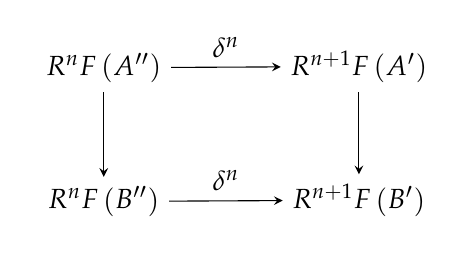
\begin{tikzpicture}
			\matrix (m) [matrix of math nodes,row sep=3em,column sep=4em,minimum width=2em]
			{
				R^nF\left(A''\right) & R^{n+1}F\left(A'\right)\\ 
				R^nF\left(B''\right) & R^{n+1}F\left(B'\right)\\};
			\path[-stealth]
			(m-1-1) edge node [above] {$\delta^n$} (m-1-2)
			(m-2-1) edge node [above]  {$\delta^n$} (m-2-2)
			(m-1-1) edge node [right]  {} (m-2-1)
			(m-1-2) edge node [right] {} (m-2-2);
		\end{tikzpicture}
		\\
		\	
		\item[(e)] For each injective object $I$ of $\mathfrak A$, and for each $n \ge 0$, we have $R^nF\left(I\right)= 0$.
		
	\end{enumerate}
\end{theorem}
\begin{definition}\label{acyc_defn}\cite{hartshorne:ag}
With 	$F: \mathfrak A \to  \mathfrak B$  as in the theorem \ref{derived_finctor_thm}, an object $J$ of $\mathfrak A$ is acyclic for 
$F$ if $R^pF = 0$ for all $p > 0$. 
\end{definition}
\begin{proposition}\label{acyc_prop}\cite{hartshorne:ag}
%Proposition 1.2A. 
With 	$F: \mathfrak A \to  \mathfrak B$  as in the theorem \ref{derived_finctor_thm}, suppose there is an exact 
sequence 
$$
0 \to A \xrightarrow{\dl_0} J^0 \xrightarrow{\dl_1}J^1 \to \dots
$$
where each $J^p$ is acyclic for $F$,  $p\ge 0$. (We say $J^\bullet$ is an $F$-\textit{acyclic resolution}
of $A$.) Then for each $p \ge 0$ there is a natural isomorphism $R^p\left( F\left(A \right) \right) = h^p\left( F\left( J^\bullet\right) \right)$
where 
	\be\label{etale_der_eqn}
	\begin{split}
h^p\left( F\left( J^\bullet\right) \right)\bydef\begin{cases}
	\ker F\left( \dl^0 \right) & p = 0\\
	\ker~ F\left(  \dl_{p} \right) / \im~ F\left(  \dl_{p-1}\right)   & p > 0
\end{cases}
	\end{split}
\ee

\end{proposition}


The complex \eqref{complex_eqn}  and the Theorem \ref{derived_finctor_thm} define the $r^{\text{th}}$ cohomology
group  $$
H^r\left(X,\ \mathscr F \right)\bydef R^r\Ga\left(X, \F \right) 
$$.
The theory of derived functors (cf. Theorem \ref{derived_finctor_thm}) shows:
\begin{enumerate}
	\item [(a)] $H^0\left(X,\ \mathscr F  \right)\cong \Ga\left(X,\ \mathscr F \right)$ for any sheaf $\mathscr F$;
	\item [(b)] if $\mathscr I$ is injective, then $H^r (X,\mathscr I )= 0$ for $r > 0$;
	\item [(c)]  short exact sequence of sheaves
	$0\to \mathscr F' \to \mathscr F \to \mathscr F'' \to 0$	gives rise to a long exact sequence
	$$
	0 \to H^0\left(X, \mathscr F'  \right) \to H^0\left(X, \mathscr F  \right) \to H^0\left(X, \mathscr F''  \right) \to H^1\left(X,\ \mathscr F'  \right) \to ...
	$$
	and the association of the long exact sequence with the short exact sequence is functional;
	\item[(d)]
	
	\be\label{etale_coh_eqn}
\begin{split}
	H^p\left(X, \mathscr F \right)\bydef\begin{cases}
		\ker \Ga\left( \dl^0 \right) & p = 0\\
		\ker~ \Ga\left(  \dl_{p} \right) / \im~ \Ga\left(  \dl_{p-1}\right)   & p > 0
	\end{cases}
\end{split}
\ee
\end{enumerate}
Moreover, the functors $H^r\left( X,~ \cdot ~\right)$  are uniquely determined (up to a unique isomorphism)
by the properties (a), (b) and (c).

\begin{proposition}\label{spectral_sequence_prop}\cite{johnstone:topos}
	%8.17 
	Let $\mathscr F \xrightarrow{f} \mathscr E$ be a geometric morphism (cf. Definition \ref{geometric_morphism_defn}) between Grothendieck toposes (cf. Definition \ref{grothendiek_topos_defn}). Then
		\begin{enumerate}		\item [(i)] 
		if $A$ is an Abelian group in $\mathscr E$ then we have a homomorphism $H^q\left(\mathscr E, A \right) \xrightarrow{} H^q \left(\mathscr F, f^*A\right)$ for each $q$ which is functorial in $f$ and natural in $A$.
			\item [(ii)] If $B$ is an Abelian group in $\mathscr F$ then we have a spectral sequence (Leray spectral sequence) $H^p\left(\mathscr E, R^qf_*\left(B \right) \right)\Rightarrow H^{p + q}\left(\mathscr F, B \right)$ which is natural in $B$.
			\end{enumerate}
\end{proposition}
	\begin{notation}\label{const_shef_coh_not}
		If  $F$ is an Abelian group and $F_X$ is a {constant presheaf} (cf. Definition \ref{constant_presheaf_defn}) then we use the following notation
		\be\label{const_shef_coh_eqn}
		\forall r\ge 0\quad H^r\left(X, F \right) \bydef H^r\left(X, \mathfrak{Ass} \left( F_X\right)  \right).
		\ee
		where $\mathfrak{Ass}$ means the associated sheaf functor (cf. Definition \ref{associated_sheaf_defn}).
	\end{notation}
	
	
	
	
	\subsection{\v{C}ech cohomology}\label{presheaf_cohomology_sec}
	\paragraph*{} Here I follow to \cite{milne:lec}. Let $\mathbf T$ be a site, and let $X$ be an object of $\mathrm{Cat}\left( \mathbf T\right)$. Let $\mathscr U \bydef \left\{U_\iota \to X\right\}_{\iota \in I}$ be  covering of $X$, and let $\mathscr P$ be a presheaf of Abelian groups. Define
	\be\label{cech_eqn}
	C^r\left( \mathscr U, \mathscr P\right)\bydef \prod_{\left(\iota_0,.... \iota_r\right) \in I^{r+1}} \mathscr P\left(U_{\iota_0,.... \iota_r} \right)\quad \text{where} \quad U_{\iota_0,.... \iota_r} \bydef U_{\iota_0}\times_X...\times_XU_{\iota_r}. 
	\ee
	For $s \in C^r\left( \mathscr U, \mathscr P\right)$ define $d^rs \in C^{r+1}\left( \mathscr U, \mathscr P\right)$ by the rule
	$$
	d^rs_{\iota_0,..., \iota_{r + 1}}\bydef \sum_{j = 0}^{r + 1}\left(-1 \right) \mathrm{res}_j\left(s_{\iota_0,..., \iota_{j-1},...,\iota_{j+1},..., \iota_{r + 1}} \right)  
	$$
	$\mathrm{res}_j$ is the restriction map corresponding to the projection map
	$$
	U_{\iota_0,..., \iota_{r + 1}}\mapsto U_{\iota_0,..., \iota_{j-1},...,\iota_{j+1},.., \iota_{r + 1}}.
	$$
	As in the classical case, one verifies by a straightforward calculation that
	$$
	C^\bullet\left( \mathscr U, \mathscr P\right) \bydef C^0\left( \mathscr U, \mathscr P\right) \to C^r\left( \mathscr U, \mathscr P\right) \xrightarrow{d_r} C^r\left( \mathscr U, \mathscr P\right)\to ...
	$$
	is a complex. Define
	\be\label{cech_coh_eqn}
	\check{H}^r\left( \mathscr U, \mathscr P\right) \bydef H^r\left(C^\bullet\left( \mathscr U, \mathscr P\right)   \right)= \begin{cases}
		\ker d_0 & r = 0\\
		\ker d_r / \im d_{r-1} & r > 0
	\end{cases}. 
	\ee
	It is called the $r^{\text{th}}$ \textit{\v{C}ech cohomology group} of $\mathscr P$ relative to the covering $\mathscr U$.
	Note that
	$$
	\check{H}^0\left( \mathscr U, \mathscr P\right)= \ker\left(\prod \mathscr P_\iota \rightrightarrows \prod \mathscr P_{\iota,j} \right) 
	$$
	Therefore, for a sheaf $\mathscr F$ one has
	$$
	\check{H}^0\left( \mathscr U, \mathscr F\right)=\Ga\left( \mathscr U, \mathscr F\right).
	$$
	A second covering $\mathscr V \bydef \left\{V_j\to X \right\}_{j \in J}$ of $X$ is called a \textit{refinement} of $\mathscr U$ if there is a
	map $\tau : J\to I$ such that $V_j \to X$ factors through $U_{\tau_j}\to X$ for all $j \in J$ . The choice of
	a $\tau$ and $X$-morphisms $\varphi_{j}: V_j \to U_{\tau_j}$ for each $j$ determines a map of complexes
	\bean
	\tau^\bullet: C^\bullet\left( \mathscr U, \mathscr P\right)\to C^\bullet\left( \mathscr V, \mathscr P\right),\\
	\left( \tau^r s_{j_0,..., j_{r}} \right) \bydef s_{\tau j_0,..., \tau j_{r}}.
	\eean
	As in the classical case, one verifies that the map on cohomology groups
	$$
	\rho \left(\mathscr U, \mathscr V \right): \check{H}^r\left( \mathscr U, \mathscr P\right)\to \check{H}^r \left( \mathscr V, \mathscr P\right)
	$$
	is independent of all choices. We may pass to the limit over all coverings, and so obtain limits
	\be\label{chech_eqn}
	\check{H}^r\left(X, \mathscr P\right)\bydef \varinjlim_{\mathscr U}\check{H}^r\left( \mathscr U, \mathscr P\right).
	\ee
	
	\begin{defn}\label{chech_defn}\cite{bryl:loop,milne:lec}
		The  \textit{\v{C}ech cohomology groups} are given by equation \eqref{chech_eqn}.
	\end{defn}
	These groups  have the following properties:
	\begin{enumerate}
		\item [(a)] $\check{H}^0\left(X, \mathscr F\right)= \Ga\left( X, \mathscr F\right)$ for any sheaf $\mathscr F$ on $X$;
		\item[(b)] $\check{H}^r\left(X, \mathscr I\right)$, $r > 0$, for all injective sheaves $\mathscr I$
	\end{enumerate}
	(cf \cite{milne:lec} for details).
	\begin{empt}
		For any Abelian group $F$ one can define a constant presheaf $F_X$ of Abelian groups (cf. Definition \ref{constant_presheaf_defn}). 
		We use a following notation
		\be\label{etale_hom_a_eqn}
		\check{H}^r\left(X, F\right)\bydef \check{H}^r\left(X, F_X\right).
		\ee
	\end{empt}
	\subsection{Set and universes}
	

	For a set $u$, we denote as usual by $\P\left( u\right)$  the set of subsets of $u : \P(u) \bydef
\left\{x | x \subset u\right\}$
\begin{definition}\cite{kashiwara:cat_sheaves}
%	Definition 1.1.1. 
	A universe $\sU$ is a set satisfying the following properties:
	\begin{enumerate}
		\item[(i)] 		$\emptyset\in \sU$
		\item[(ii)] $u \in \sU$ implies $u\subset \sU$, (equivalently, $x \in \sU$ and $y \in x$ implies $y\in \sU$, or 	else $\sU \subset \P\left( \sU\right)$ ,
		\item[(iii)] $u \in \sU$ implies $\{u\}\in \sU$,
		\item[(iv)] $u \in \sU$ implies $\P\left( u\right)  \in \sU$,
		\item[(v)] if $I \in \sU$ and $u_i\in \sU$ for all $i \in I$ , then $\bigcup_{i \in I}u_i \in \sU$
	\item[(vi)] $\N \in \sU$.
		
	\end{enumerate}
	As a consequence we have
	\begin{enumerate}
		\item[(vii)] $u \in \sU$ implies $\bigcup_{x \in u} x \in \sU$,
			\item[(viii)]$u,v \in \sU$ implies $x \times y \in \sU$,
		\item[(ix)] $u \subset v \in \sU$ implies $u \in \sU$,
		\item[(x)] if $I \in \sU$ and $u_i \in \sU$ for all $i \in I$, then $\prod_{i \in I} u_i \in \sU$.
	\end{enumerate}
	Following Grothendieck, we shall add an axiom to the Zermelo-Fraenkel theory,
asking that for any set $X$ there exists a universe $\sU$ such that $X \in \sU$.
\end{definition}
\begin{definition}\cite{kashiwara:cat_sheaves}
%Definition 1.1.2. 
Let $\sU$ be a universe.
\begin{enumerate}
	\item [(i)] A set is called a $\sU$-\textit{set} if it belongs to $\sU$.
	\item [(ii)] A set is called $\sU$-\textit{small} if it is isomorphic to a set belonging to $\sU$.
\end{enumerate}
\end{definition}
\begin{definition}
A category $\mathscr C$ is called a $\sU$-\textit{category} if $\Hom \mathscr C(X, Y)$ is $\sU$-small for any $\mathscr C$-objects $X$ and $Y$.
\end{definition}

\begin{definition}
%Definition 1.4.2. 
Let $\mathscr C$ be a $\sU$-category. We define the big categories
\bean
\mathscr C^\wedge_\sU \bydef  \text{ the category of functors from } \mathscr C^{\mathrm{op}} \text{ to } \sU\text{-}\mathbf{Set} ,\\
\mathscr C^\vee_\sU \bydef  \text{ the category of functors from } \mathscr C^{\mathrm{op}} \text{ to } \left( \sU\text{-}\mathbf{Set}\right)^{\mathrm{op}} 
\eean 
and the functors
\bean
\mathrm{h}_{\mathscr C}: \mathscr C\to \mathscr \mathscr C^\wedge_\sU\quad X \mapsto \Hom\left(\bullet, X \right),\\ 
\mathrm{k}_{\mathscr C}: \mathscr C\to \mathscr \mathscr C^\vee_\sU\quad X \mapsto \Hom\left( X, \bullet \right)
\eean 

\end{definition}
\begin{definition}
A category $I$ is \textit{filtrant} if it satisfies the conditions (i)�(iii)
below.
\begin{enumerate}
	\item [(i)] $I$ is non empty,
	\item [(ii)]  for any $i$ and $j$ in $I$ , there exist $k \in I$ and morphisms $i \to k$, $j \to k$,
	\item [(ii)]  for any parallel morphisms $f, g : i \rightrightarrows j $, there exists a morphism $h : j \to k$
	such that $h \circ f = h \circ g$.
\end{enumerate}
A category $I$ is \textit{cofiltrant} if $I^{\mathrm{op}}$ is filtrant.
\end{definition} 
Assume first that $\mathscr C$ is the category $\mathbf{Set}$ and let us consider \textit{projective
systems}. In other words, $\bt$ is an object of $I^\wedge$. Denote by $\mathrm{pt}_{I^\wedge}$ the constant
functor from $I^\mathrm{op}$ to $\mathbf{Set}$, defined by $\mathrm{pt}_{I^\wedge}(i) \bydef \mathrm{pt}$ for all $i \in I$ . Note that $\mathrm{pt}_{I^\wedge}(i)$
is a terminal object of $I^\wedge$. We define a set, called the \textit{projective} limit of $\bt$, by
$$
\varprojlim \bt \bydef \Hom_{I^\wedge}\left(\mathrm{pt}_{I^\wedge}, \bt \right) 
$$
\begin{definition}
%Definition 2.1.2. (i)
\begin{enumerate}
	\item [(i)] We define $\varinjlim \a$ and $\varprojlim \bt$ by the formulas
	\bea
	\varinjlim \a \bydef X \mapsto \varinjlim \Hom_{\mathscr{C}}\left(\a , X  \right) = \varinjlim \left(\mathrm{h}_{\mathscr{C}}\circ \a \right) \in \mathbf{Set},\\
	\varprojlim \a \bydef X \mapsto \varprojlim \Hom_{\mathscr{C}}\left( X, b  \right) = \varprojlim \left(\mathrm{k}_{\mathscr{C}}\circ \a \right) \in \mathbf{Set}.
	\eea
\end{enumerate} 

\end{definition}

\begin{proposition}
%Proposition 3.1.3. 

Let $\a : I \to \mathbf{ Set}$ be a functor with $I$ small and filtrant.
Define the relation $\sim$ on $\coprod_i \a\left( i\right)$  as follows: $\a(i)) \ni  x \sim y \in \a( j )$ if there exist
$s : i \to k$ and $t : j \to k$ such that $\a(s)(x) = \a(t)(y)$. Then
\begin{itemize}
	\item [(i)] the relation $\sim$ is an equivalence relation,
\item	[(ii)] $\varinjlim \a = \coprod_i \a(i)/ \sim$.
\end{itemize}

\end{proposition}
	Recall that a universe $\sU$ is given. When we consider a category, it means a
	$\sU$-category and $\mathbf{Set}$ is the category of $\sU$-sets %(see Convention 1.4.1). 
	As far
	as this has no implications, we will skip this point.
	Recall that for a category $\mathscr C$, inductive limits in $\mathscr C^\wedge \bydef \bydef \mathrm{Fct}\left( \mathscr C^{\mathrm{op}}, \mathbf{Set}\right)$  are
	denoted by �$\varinjlim$�.
	\begin{definition}
	%	Definition 6.1.1.
	\begin{enumerate}
		\item[(i)] 	Let $\mathscr C$ be a $\sU$-category. An \textit{ind}-\textit{object} in $\mathscr C$ is an object
		$A \in \mathscr C^\wedge$ which is isomorphic to �$\varinjlim$� for some functor $\a : I \to  \mathscr C$  with
		$I$ filtrant and $\sU$-small.
		\item[(ii)] We denote by $\mathrm {Ind}^\sU\left(  \mathscr C \right)$ (or simply $\mathrm {Ind}\left(  \mathscr C \right)$ if there is no risk of confusion)
		the full big subcategory of $\mathscr C^\wedge$ consisting of ind-objects, and call it the \textit{indization}
		of $\mathscr C$. We denote by $\iota_{\mathscr C} : \mathscr C \to {Ind}\left(  \mathscr C \right)$ the natural functor (induced
		by $\mathrm{h}_{\mathscr C}$).
				\item[(iii)] 	Similarly a \textit{pro}-\textit{object} in $\mathscr C$ is an object
		$B \in \mathscr C^\vee$ which is isomorphic to �$\varprojlim$� $\bt$ for some functor $\bt : I^{\mathrm{op}} \to  \mathscr C$  with
		$I$ filtrant and $\sU$-small.
		\item[(iv)] We denote by $\mathrm {Pro}^\sU\left(  \mathscr C \right)$ (or simply $\mathrm {Pro}\left(  \mathscr C \right)$)
		the full big subcategory of $\mathscr C^\vee$ consisting of pro-objects
		
	\end{enumerate}
	\end{definition}
	There is an equivalence
	\be
	\mathrm {Pro}\left(  \mathscr C \right)= \mathrm {Ind}\left(  \mathscr C^{\mathrm{op}} \right)^{\mathrm{op}}
	\ee
%	Lemma 6.1.2. The categories Ind(C) and Pro(C) are U-categories.

	
	\section{Topological sheaves and cosheaves}
		\subsection{General topology}
	
	\begin{definition}\label{top_paracompact_defn}\cite{munkres:topology}
		A space $\sX$ is \textit{paracompact} if every open covering $\sX = \cup~\sU_{   \a}$ has a locally finite open refinement $\sX = \cup~\sV_{   \bt}$.
	\end{definition}
	
	\begin{lemma}
		%	'Lemma 41.6.
		
		Let $\sX$ be a paracompact Hausdorff space; let $\left\{\sU_\a\right\}$ be an  
		indexed family of open sets covering $\sX$. Then there exists a locally finite indexed family $\left\{\sV_\a\right\}$
		of open sets covering $\sX$ such that for each $\a$ the closure of $\sV_\a$ is a subset of $\sU_\a$.
	\end{lemma}
	
	\subsection{General theory of sheves}
	\paragraph*{}
	The explained below definitions are specializations of   \ref{etale_presheaf_defn} and  \ref{etale_sheaf_defn} ones (cf. Example \ref{top_gro_exm}).
	\begin{definition}\label{presheaf_defn}\cite{hartshorne:ag}
		Let $\sX$ be a topological space. A \textit{presheaf} $\mathscr F$ of Abelian groups on  $\sX$ consists of the data:
		\begin{itemize}
			\item[(a)] for every open subset $\sU \subseteq \sX$, an Abelian group $\mathscr F\left(\sU\right)$, and 
			\item[(b)] for every inclusion $\sV \subseteq \sU$ of open subsets of $\sX$, a morphism of Abelian groups $\rho_{\sU \sV}:\mathscr F\left(\sU\right) \to \mathscr F\left(\sV\right)$,\\
			subject to conditions
			\begin{itemize}
				\item [(0)] $\mathscr F\left(\emptyset \right)= 0$, where $\emptyset$ is the empty set,
				\item[(1)] $\rho_{\sU \sU}$ is the identity map, and
				\item[(2)] if $\mathcal W \subseteq \sV \subseteq \sU$ are three open sets, then $\rho_{\sU \mathcal W} = \rho_{\sV \mathcal W }\circ \rho_{\sU \sV}$.
			\end{itemize}
		\end{itemize}
	\end{definition}
	
	\begin{definition}\label{sheaf_defn}\cite{hartshorne:ag}
		A {presheaf} $\mathscr F$ on  
		a topological space $\sX$ is a \textit{sheaf}  if it satisfies the following supplementary conditions:
		\begin{itemize}
			\item[(3)] If $\sU$ is an open set, and if $\left\{\sV_{\a}\right\}$ is an open covering of $\sU$, and if $s \in \mathscr F\left(\sU\right)$ is an element such that $\left.s\right|_{\sV_{\a}}= 0$ for all $\a$, then $s = 0$;
			\item[(4)] If $\sU$ is an open set, if $\left\{\sV_{\a}\right\}$ is an open covering of $\sU$ (i.e. $\sU = \cup\sV_\a$), and we have elements $s_\a$ for each $\a$, with property that for each $\al, \bt, \left.s_\a\right|_{\sV_{\a}\cap \sV_{\bt}}= \left.s_\bt\right|_{\sV_{\a}\cap \sV_{\bt}}$, then there is an element $s \in \mathscr F\left(\sU\right)$ such that $\left.s\right|_{\sV_\a} = s_\a$ for each $\a$.
		\end{itemize}
		(Note condition (3) implies that $s$ is unique).
	\end{definition}
	
	
	
	%\begin{definition}
	%	A presheaf \ref{top_x_sheaf_defn} satisfying (4) of the Definition \ref{sheaf_defn} is called \textit{conjunctive} (for $\sU$). (cf. \cite{bredon:sheaf})
	%\end{definition}
	\begin{definition}\label{stalk_defn}\cite{hartshorne:ag}
		If $\mathscr F$ is a {presheaf} on $\sX$, and if $x$ is a point of $\sX$ we define the \textit{stalk} or the \textit{germ} $\mathscr F_x$ of $\mathscr F$ at $x$ to be the direct limit of groups $\mathscr F\left(\sU\right)$ for all open sets $\sU$ containing $x$, via restriction maps $\rho$.
	\end{definition}
	
	
	
%	\begin{prdf}\label{sheaf_prdf}\cite{hartshorne:ag}
%		Given a presheaf $\mathscr F$, there is a sheaf  $\mathscr F^+$ and a morphism $\th: \mathscr F \to \mathscr F^+$, with the property that for any sheaf  $\mathscr G$, and any morphism $\varphi: \mathscr F \to \mathscr G$, there is a unique morphism $\psi:\mathscr F^+\to \mathscr G$ such that $\varphi = \psi \circ \th$. Furthermore the pair $\left(\mathscr F^+, \th\right)$ is unique up to unique isomorphism. $\mathscr F^+$ is called the $\mathrm{sheaf~associated}$ to the presheaf $\mathscr F$. 
%	\end{prdf}
%	\begin{remark}
%		The above Proposition is a specialization of the Statement \ref{site_enough_stmt}.
%	\end{remark}
	
	\begin{definition}\label{sheaf_inv_im_defn}\cite{hartshorne:ag}
		Let $f: \sX\to \sY$ be a continuous map of topological spaces. For any sheaf  $\mathscr F$ on $\sX$, we define the \textit{direct image} sheaf  $f_*\mathscr F$ on $\sY$ by $\left(f_*\mathscr F\right)\left(\sV\right)= \mathscr F\left(f^{-1}\left(\sV\right)\right)$ for any open set $\sV \subseteq \sY$. For any sheaf  $\mathscr G$ on $\sY$, we define the \textit{inverse image} sheaf  $f^{*}\mathscr G$ on $\sX$ be the sheaf  associated to the presheaf  $\sU \mapsto \lim_{\sV \supseteq f\left(\sU\right)} \mathscr G\left(\sV\right)$, where $\sU$ is any open set in $\sX$, and the limit is taken over all open sets $\sV$ of $\sV$ containing $f\left(\sU\right)$.
	\end{definition}
	
	\begin{remark}\label{geometric_morphism_rem}\cite{johnstone:topos}
		%1.17
		If $f : \sX \to \sY$ is a continuous map then a given by the Definition \ref{sheaf_inv_im_defn} pair  of functors $f_*$ and $f^{*}$ rise a geometric morphism (cf. Definition \ref{geometric_morphism_defn}) $\mathbf{Sh}\left(\sX\right)\to \mathbf{Sh}\left(\sY\right)$ between categories of sheaves. 
	\end{remark}
	\begin{exercise}\label{dir_image_exer}
		Let $f : \sX \to \sY$ be a continuous map, and let $F$ be a set. Prove that if  	both $F_\sX$ and $F_\sY$ are constant presheaves  (cf. Definition \ref{constant_presheaf_defn}) on $\sX$ and $\sY$ 
		then one has:
		\begin{enumerate}
			\item there is a natural isomorphism of sheaves
			\bean\label{dir_image_eqn}
			\mathfrak{Ass}\left( F_\sY\right) \cong f_*\mathfrak{Ass}\left( F_\sX\right)
			\eean
			where 
			$\mathfrak{Ass}$  means the associated sheaf functor (cf. Definition \ref{associated_sheaf_defn}) and 	
			$f_*$ means the direct image (cf. Definition \ref{sheaf_inv_im_defn}),
			\item if $f$ is a local homeomorphism then there is a natural isomorphism of sheaves
			\be\label{inv_image_eqn}
			\mathfrak{Ass}\left( F_\sX\right) \cong f^*\mathfrak{Ass}\left( F_\sY\right)
			\ee
			where	$f^*$ means the  inverse image (cf. Definition \ref{sheaf_inv_im_defn}).
		\end{enumerate}
	\end{exercise}
%	\begin{definition}\label{sheaf_morphism_defn}\cite{hartshorne:ag}
%		If $\mathscr F$  and $\mathscr G$ are presheaves on $\sX$, a \textit{morphism} $\varphi:\mathscr F\to\mathscr G$  consists 		of a morphism of Abelian groups $\varphi_\sU:\mathscr F\left( \sU\right) \to\mathscr F\left( \sU\right)$ for each open set 		$\sU$, such that whenever $\sV\subset\sU$ is an inclusion, the diagram 
%		\newline
%		\begin{tikzpicture}
%			\matrix (m) [matrix of math nodes,row sep=3em,column sep=4em,minimum width=2em]
%			{
%				\mathscr F\left( \sU\right)   & \mathscr G\left( \sU\right)\\
%				\mathscr F\left( \sV\right)    & \mathscr G\left( \sV\right)\\
%			};
%			\path[-stealth]
%			(m-1-1) edge node [above] {$\rho_{\sU\sV}$} (m-1-2)
%			(m-1-1) edge node [right] {$\varphi_\sU$} (m-2-1)
%			(m-1-2) edge node [right] {$\varphi_\sV$} (m-2-2)
%			(m-2-1) edge node [above] {$\rho'_{\sU\sV}$} (m-2-2);
%		\end{tikzpicture}
%		\\
%		is commutative, where $\rho_{\sU\sV}$ and $\rho'_{\sU\sV}$ are the restriction maps in $\mathscr F$  and $\mathscr G$. If $\mathscr F$  and $\mathscr G$ are sheaves on $\sX$, we use the same definition for a morphism 
%		of sheaves. An isomorphism is a morphism  which has a two-sided inverse. 
%	\end{definition}
%	\begin{empt}\label{open_sheaf_empt}
%		For any topological space $\sX$ there is a \textit{sheaf of stalks of open sets} $\Om_\sX$ on $\sX$ (cf. \cite{goldblatt:topoi})		such that
%		\bean
%		\Om_\sX \left(\sU \right)  \bydef  \text{the family of all open subsets of }\sU;\\
%		\rho_{\sU \sV}: \Om_\sX\left(\sU \right) \to \Om_\sX\left(\sV \right), \quad \mathcal W \mapsto \mathcal W \cap \sV.
%		\eean
%	\end{empt}
\begin{empt}\label{sheaf_empt}
	Following text is the citation of the proof of \ref{sheaf_prdf} (cf. \cite{hartshorne:ag}). For any open set $\sU$, let $\mathscr F^+\left(\sU\right)$ be set of functions $s$ from $\sU$ to the union $\bigcup_{x \in \sU}  \mathscr F_x$ of stalks of $\mathscr F$ over points of $\sU$, such that
	\begin{itemize}
		\item [(1)] for each $x \in \sU$, $s\left(x\right)\in \mathscr F_x$, and
		\item[(2)] for each $x \in \sU$, there is a neighborhood $\sV$ of $x$ contained in $\sU$ and an element $t \in \mathscr F\left(\sV\right)$, such that for all $y \in \sV$ the stalk (germ) $t_y$ of $t$ at $y$ is equal to $s\left(y\right)$.
	\end{itemize}
\end{empt}

\begin{exercise}\label{sheaf_etale_exer}\cite{hartshorne:ag}
	%1.13. 
	\textit{
		\'Espace Etal\'e of a Presheaf}. %(This exercise is included only to establish the connection between our definition of a sheaf and another definition often found in the literature. See for example Godement [1, Ch. II, �1.2].)
	Given a presheaf $\mathscr F$ on $\sX$, we define a topological space $\mathrm{Sp\acute{e}}\left(\mathscr F \right)$ , called the \textit{
		\'espace etal\'e} of a presheaf of $\mathscr F$ as 
	follows. As a set, $\mathrm{Sp\acute{e}}\left(\mathscr F \right)= \bigcup_{x\in\sX} \mathscr F_x$. We define a projection map $p: \mathrm{Sp\acute{e}}\left(\mathscr F \right)\to \sX$
	by sending $s_x\in \mathscr F_x$ to $x$. For each open set $\sU\subset\sX$ and each section $s\in \mathscr F\left(\sU \right)$  we 
	obtain a map: $\overline{s}: \sU \to  \mathrm{Sp\acute{e}}\left(\mathscr F \right)$ by sending $x \mapsto s_x$, its germ at $x$. This map has the property that 
	$p\circ \overline{s}= \Id_\sX$, in other words, it is a "section" of $p$ over $\sU$. We now 
	make $\mathrm{Sp\acute{e}}\left(\mathscr F \right)$ into a topological space by giving it the strongest topology such that 
	all the maps $\overline{s}: \sU \to  \mathrm{Sp\acute{e}}\left(\mathscr F \right)$ for all $\sU$ and all $s\in \mathscr F\left(\sU \right)$ , are continuous. Now 	show that the sheaf $\mathscr F^+$ associated to $\mathscr F$ can be described as follows: for any 
	open set $\sU\subset \mathscr F$, $\mathscr F\left(\sU \right)$ is the set of continuous sections of $\mathrm{Sp\acute{e}}\left(\mathscr F \right)$ over $\sU$. In 
	particular, the original presheaf $\mathscr F$ was a sheaf if and only if for each $\sU\subset \sX$,  $\mathscr F\left(\sU \right)$ is 
	equal to the set of all continuous sections of $\mathrm{Sp\acute{e}}\left(\mathscr F \right)$ over $\sU$. 
	
\end{exercise}



\begin{remark}\label{sheaf_rem}\cite{bredon:sheaf, godement:sheaf}	
	If $\sV \subset \sX$ is any subset  then  one can define a group $\mathscr F\left(\sV\right)$  which is a group of continuous maps  $\iota :\sV\to \mathrm{Sp\acute{e}}\left(\mathscr F \right)$ such that $p\circ\iota = \Id_\sV$. Denote by  $\mathscr F\left(\sV \right)$ the Abelian group of such maps.
\end{remark}
\begin{empt}\cite{bredon:sheaf, godement:sheaf}					
 For any sheaf $\mathscr F$ of Abelian groups on $\sX$ and open set $\sU\subset \sX$  we let $C^0(\left(\sU, \mathscr F \right)$ be the
	collection of all functions (not necessarily continuous) $f: \sU\to \mathrm{Sp\acute{e}}\left(\mathscr F \right)$ such 	that $p \circ f$ is the identity on $\sU$, $~~p : \mathrm{Sp\acute{e}}\left(\mathscr F \right)\to \sX$ being the canonical projection (cf. Exercise \ref{sheaf_etale_exer}).
	Such possibly discontinuous sections are called \textit{serrations}. That is
	\be
	C^0(\left(\sU, \mathscr F \right)\bydef \prod_{x \in \sX} \mathscr F_x
	\ee
	!!! WHERE $F_x$ !!!
	Under point-wise operations, this is an Abelian group, and the functor $\sU \mapsto 	C^0(\left(\sU, \mathscr F \right)$, $\sX$. Indeed it is a sheaf (cf. \cite{bredon:sheaf}) which will be denoted by $\mathscr C^0(\left(\sU, \mathscr F \right)$. Note that if $\sX_d$ denotes the point set of $\sX$ 
	with the discrete topology and if $\phi : \sX_d \to \sX$ is the canonical map, then $\mathscr C^0(\left(\sU, \mathscr F \right)\cong f_*f^* \mathscr F$.
	Inclusion of the collection of sections of $\mathscr F$ in the collection of all serrations
	gives an inclusion $\mathscr F\left(\sU \right)\mapsto   C^0(\left(\sU, \mathscr F \right)= \mathscr C^0(\left(\sU, \mathscr F \right)\left(\sU \right)$  and hence
	provides a natural monomorphism
	\be\label{sheaf_can_res}
	\eps : \mathscr F \hookto \mathscr C^0\left(\sX, \mathscr F \right)
	\ee
	(For $\phi : \sX_d \to \sX$ as above, this inclusion coincides with the monomorphism
	$\bt :\mathscr F \hookto f_*f^*\mathscr F$). 
	Let $\mathscr{Z}^{1}\left(\sX, \mathscr F \right) \bydef \coker\left\{\mathscr F \hookto \mathscr C^0\left(\sX, \mathscr F \right)\right\}$. so that the sequence
	$$
	\{0\}\to \mathscr F \to \mathscr{C}^{0}\left(\sX, \mathscr F \right) \to \mathscr{Z}^{1}\left(\sX, \mathscr F \right)\to {0}
	$$
	is exact. We also define, inductively,
\bean
	\mathscr{C}^{n}\left(\sX, \mathscr F \right) \bydef \mathscr{C}^{0}\left( \mathscr{Z}^{n}\left(\sX, \mathscr F \right)\right),\\
	\mathscr{Z}^{n+1}\left(\sX, \mathscr F \right) \bydef \mathscr{Z}^{1}\left( \mathscr{Z}^{n}\left(\sX, \mathscr F \right)\right)  
\eean
	so that
\bean
		\mathscr{Z}^{n}\left(\sX, \mathscr F \right) \xrightarrow{\eps} \mathscr{C}^{n}\left(\sX, \mathscr F \right)\xrightarrow{\partial}
	\mathscr{Z}^{n+1}\left(\sX, \mathscr F \right)
\eean

	is exact. Let $d \bydef \eps \circ \partial$ be the composition
	$$
	\mathscr{C}^{n}\left(\sX, \mathscr F \right) \xrightarrow{\partial }  \mathscr{Z}^{n + 1}\left(\sX, \mathscr F \right)\xrightarrow{\eps}\mathscr{C}^{n+1}\left(\sX, \mathscr F \right) 
$$

	Then the sequence 
	\be
0 \to \mathscr F \xrightarrow{\eps} 	\mathscr{C}^{0}\left(\sX, \mathscr F \right) \xrightarrow{d } \mathscr{C}^{1}\left(\sX, \mathscr F \right)\xrightarrow{d } \mathscr{C}^{2}\left(\sX, \mathscr F \right)\xrightarrow{d}\dots
	\ee
	is exact. That is, $\mathscr{C}^{\bullet}\left(\sX, \mathscr F \right)$ is a resolution of $\mathscr F$. It is called the \textit{canonical
	resolution} of $\mathscr F$.
\end{empt}

\begin{definition}\label{sub_sheaf_defn}\cite{hartshorne:ag}
	A \textit{subsheaf}  of a sheaf $\mathscr F$ is a sheaf $\mathscr F'$ such that for every open set 
	$\sU \subset \sX$, $\quad \mathscr F'\left(\sU \right)$  is a subgroup of $\mathscr F\left(\sU \right)$, and the restriction maps of the 
	sheaf $\mathscr F'$ are induced by those of $\mathscr F$. It follows that for any point $P$, the 
	stalk $\mathscr F'_P$ is a subgroup of $\mathscr F_P$. 
	%If (p: & -> ^ is a morphism of sheaves, we define the fce/w/ of (p, denoted ker cp, to be the presheaf kernel of cp (which is a sheaf). Thus ker cp is a subsheaf of .^. We say that a morphism of sheaves cp:^ -> (^ is injeetive if ker (p = 0. Thus <p is injeetive if and only if the induced map cp{U)\^(U) -> ^(G) is 	injeetive for every open set of X. 	If cp\ 3F -> ^ is a morphism of sheaves, we define the zm^ of cp, 	denoted im cp, to be the sheaf associated to the presheaf image of cp. By 	the universal property of the sheaf associated to a presheaf, there is a 	natural map im cp -> rS. In fact this map is injeetive (see Ex. 1.4), and thus 	im cp can be identified with a subsheaf of f&. 	We say that a morphism cp\, -> ^ of sheaves is sitrjective if im cp = f^. 	We say that a sequence . . . �> ^l~"] -�> .Wl ^> ,l^x -> . . . of sheaves 	and morphisms is ^xacr if at each stage ker <p' = im cpl ~ l. Thus a sequence
		
	\end{definition}
	
	
	\begin{definition}\label{sheaf_hom_defn}\cite{hartshorne:ag}
		Let $\mathscr F$, $\mathscr G$ be sheaves of Abelian  groups  on $\sX$. For any open set $\sU \subseteq \sX$ the set of morphisms
		$\Hom\left(\left.\mathscr F\right|_{\sU}, \left.\mathscr G\right|_{\sU}\right)$ has the natural structure of Abelian group. 
		It is a sheaf  (cf. \cite{hartshorne:ag}). It is called the \textit{sheaf of local morphisms} of $\mathscr F\to \mathscr G$, "sheaf hom" for short, and is denoted by $\mathscr Hom \left(\mathscr F, \mathscr G\right)$.
	\end{definition}
	
	\begin{definition}\label{sheaf_ringed_space_defn}\cite{hartshorne:ag}
		A \textit{ringed space} is a pair $\left(\sX, \mathcal O_\sX \right)$  consisting of a topological space 
		$\sX$ and a sheaf of rings $\mathcal O_\sX$  on $\sX$.
		% A morphism of ringed spaces from (X,CX) to (Y,GY) is a pair (./,/#) of a continuous map f:X-+ Y and a map f# :(ry -> fJ9x of sheaves of rings on Y. The ringed space (X,x) is a locally ringed space if for each point P e X, the stalk ([x P is a local ring. A morphism of locally ringed spaces is a morphism (/,/#) of ringed spaces, such that for each point P e X, the induced map (see below) of local rings fp :Cyj(P) -+ x,p ls a lcal homomorphism of local rings. We explain this last condition. First of all, given a point P e X, the morphism of sheaves f*:((Y -+ l\fix induces a homomorphism of rings CY(V) -> x(f~ { V), for every open set V in Y. As V ranges over all open neighbor- 	hoods of /(P), f~l(V) ranges over a subset of the neighborhoods of P. 	Taking direct limits, we obtain a map 	&YJ{P) = \jmCY(V)^\jme>'x(f-1V), 		72 
				
			\end{definition}
			
			\begin{definition}\label{sheaf_of_modules_den}\cite{hartshorne:ag}
				Let $\left(\sX, \mathcal O_\sX \right)$  be a ringed space. A \textit{sheaf  of $ \mathcal O_\sX $-modules} 
				(or simply an $\mathcal O_\sX$ -\textit{module}) is a sheaf  $\mathscr F$ on $\sX$, such that for each open set 
				$\sU\subset\sX$, the group 
				$\mathscr F\left(\sU \right)$ is an $\mathcal O_\sX$-module, and for each inclusion of 
				open sets $\sV \subset\sU$, the restriction homomorphism $\mathscr F\left(\sU \right) \to \mathscr F\left(\sV \right)$  is compatible with the module structures via the ring homomorphism $\mathcal O_\sX\left(\sU \right) \to \mathcal O_\sX \left(\sV \right)$.
				%	(9X(V). A morphism #" �> ^ of sheaves of $x-modules is a morphism of 
				%	sheaves, such that for each open set U ^ X, the map <F(U) -> ^(7) is a 
				%	homomorphism of $x(L/)-modules. 	Note that the kernel, cokernel, and image of a morphism of 6rx-modules 	is again an Gx-modu\e. If ^'ls a subsheaf  \ref{top_x_sheaf_defn} of (^'x-modules of an (9x-modu\e 	#", then the quotient sheaf \ref{top_x_sheaf_defn} gFj^F' is an #x-module. Any direct sum, 	direct product, direct limit, or inverse limit of $x-modules is an $x-module. 	If J^ and ^ are two $x-modules, we denote the group of morphisms from 	^ to ^ by Hom^^,^), or sometimes Homx(J^) or Hom( J^) if no 	conncsion can arise. A sequence of $x-modules and morphisms is exact 	if it is exact as a sequence of sheaves of abelian groups. 	If U is an open subset of X, and if J^ is an $x-module, then tF\v is an 	(9x\v-modu\e. If 3F and ^ are two ^x-modules, the presheaf  \ref{top_x_sheaf_defn} 	is a sheaf, which we call the sheaf  \ref{top_x_sheaf_defn} Worn (Ex. 1.15), and denote by 	.^bm^l^). It is also an $x-module. 
			\end{definition}
					
			\subsection{Flasque (flabby) and soft sheaves}
			\begin{definition}\label{sheaf_flasque_defn}\cite{hartshorne:ag}
				A sheaf  $\mathscr F$ on a topological space is \textit{flasque} or \textit{flabby} if for every inclusion $\sV \subseteq \sU$ of open sets, the restriction map $\mathscr F\left(\sU \right)\to\mathscr F\left(\sV \right)$ is surjective. 
			\end{definition}
			\begin{remark}\label{sheaf_locale_flasque}
			If $X$ ia a locale then one can define flasque sheaves in the category $\mathbf{Sh}\left(X \right)$. 
			\end{remark}
			\begin{proposition}\label{sheaf_flasque_prop}\cite{hartshorne:ag}
			%Proposition 2.5. // 
		If $\mathscr F$ is a flasque sheaf on a topological space $\sX$, then  $H^p\left(\sX, \mathscr F \right)  = 0$ for all $p > 0$.
			\end{proposition}
			\begin{exercise}\label{sheaf_flasque_exer}
			Similarly to the described in \cite{hartshorne:ag} theory of flasque shaves prove that
			for any locale $X$ and for every flasque sheaf in the category $\mathbf{Ab}\left(X \right)$ one has  $H^p\left(X, \mathscr F \right)  = 0$ for all $p > 0$ 
			\end{exercise}
		\begin{remark}\label{sheaf_flasque_rem}
	If $X$ is   a locale, $\mathscr F \in \mathbf{Ab}\left(X \right)$ and 
		$$
		0 \to \mathscr F \xrightarrow{\dl_0} \sJ^0 \xrightarrow{\dl_1}\sJ^1 \to \dots
		$$
		is an exact sequence where each $\sJ^p$ is flasque then from the Exercise \ref{sheaf_flasque_exer} it follows that $\sJ^p$ is acyclic for any $p\ge 0$. Taking into account the Proposition \ref{acyc_prop} one has
			\be\label{etale_cohf_eqn}
		\begin{split}
			H^p\left(X, \mathscr F \right)\bydef\begin{cases}
				\ker \Ga\left( \dl^0 \right) & p = 0\\
				\ker~ \Ga\left(  \dl_{p} \right) / \im~ \Ga\left(  \dl_{p-1}\right)   & p > 0
			\end{cases}
		\end{split}
		\ee
		\end{remark}	
			Recall that for $s \in \mathscr{F}\left(\sX \right)$, 
			\be\label{sheaf_supp_eqn}
			\supp s= \left\{\left.x \in \sX \right|s\left(x \right)\neq 0  \right\}
			\ee
			denotes the \textit{support} of the section $s$.
			\begin{definition}\label{phi_supp_defn}\cite{godement:sheaf}.
				Let $\sX$ be a topological space. A \textit{family of supports} on $\sX$ is a family $\Phi$ of closed
				subsets of $\sX$  such that:
				\begin{enumerate}
					\item a closed subset of a member of $\Phi$ is a member of $\Phi$;
					\item $\Phi$ is closed under finite unions.
				\end{enumerate}
				
				$\Phi$  is said to be a  \textit{paracompactifying} family of supports if in addition:
				\begin{enumerate}
					\item  each element of $\Phi$ is paracompact;
					\item each element of $\Phi$ has a (closed) neighborhood which is in $\Phi$.
				\end{enumerate}
			\end{definition}\label{sheaf_soft_defn}
			The family of all compact subsets of $\sX$ is denoted by $c$.
			\begin{definition}\label{soft_sheaf_defn}\cite{bredon:sheaf}
				A sheaf  $\mathscr{F}$ on $\sX$ is called $\Phi$-\textit{soft} if the restriction map	$\mathscr{F}\left(\sX \right) \to  \mathscr{F}\left(K \right)$  is surjective for all $K \in \Phi$. If $\Phi$ is a set of all closed sets  then $\Phi$ is simply
				called \textit{soft}. If $\Phi= c$ is a set of all compact  sets  then $\mathscr{F}$ is called $c$-\textit{soft}.
			\end{definition}
	Now  $\mathscr P$ is a presheaf  on $\sX$ such and $s \in \mathscr P\left(\sX \right)$ we put
			$\left|s\right| = \left|\th\left( s\right) \right|$, where $\th: \mathscr{P}\left(\sX \right)\to \mathscr{P}^+\left(\sX \right) $ is the canonical map, $\mathscr{P}^+$ being the sheaf  generated by $\mathscr{P}$.
			Note that for $s \in \mathscr{P}$ one has $x \notin \left|s\right|\Leftrightarrow\left.s \right|_{\sU}=0$ for some neighborhood $\sU$ of $x$. If $\mathscr{F}$ is a sheaf, we put
			$$
			\Ga_\Phi = \left\{\left.s\in \mathscr{F}\left( \sX\right)\right| \left|s\right| \in \Phi \right\}.
			$$
			
				
			For a presheaf $\mathscr{P}$  on $\sX$ we put  $\mathscr{P}_\Phi\left(\sX \right) = \left\{\left.s\in \mathscr{P}\left( \sX\right)\right| \left|s\right| \in \Phi \right\}$.
			\begin{lemma}\label{schv_soft_n_lem}\cite{godement:sheaf,torsten:sheaves}
				Let $\sX$ be a paracompact space, $\mathscr{F}$ a sheaf on $\sX$. Then $\mathscr{F}$ is soft if and only if every point $x \in \sX$ has a closed neighborhood $\overline{   \mathcal U }$ such that $\left.\mathscr{F}\right|_{\overline{   \mathcal U }}$ is soft.
			\end{lemma}
			
			
			%\begin{theorem}\cite{bredon:sheaf}
			%	6.2.\\
			%	Theorem. Let $\mathscr P$ be a presheaf  DEFN \ref{top_x_sheaf_defn} on $\sX$ that is conjunctive for coverings	of $\sX$ and $\mathscr P^+$ be the sheaf \ref{top_x_sheaf_defn} generated by $\mathscr P$. Then for any paracompactifying 	family $\Phi$ of supports on $\sX$, the sequence
			%	$$
			%	0 \to \mathscr P_0\left( \right) \to  \mathscr{P}_\Phi\left(\sX \right) \xrightarrow{\th}\Ga_\Phi\left(\mathscr{P}^+ \right) 
			%	$$
			%	is exact.
			%\end{theorem}
			\begin{theorem}\label{sheaf_neigh_thm}\cite{godement:sheaf}
				%	3.3.1\\
				Let $\mathscr{F}$ be a sheaf  of set over the space $\sX$, $\mathcal S$ is a subset of $\sX$ and $s$ is a section of the sheaf  $\mathscr{F}$ over $\mathcal S$. If $\mathcal S$ allows a fundamental system of paracompact neighborhoods then $s$ can be extended to a neighborhood of $\mathcal S$ in $\sX$. 
			\end{theorem}
			\begin{theorem}
				%Thorme 3.4.1- � 
				Soit $\mathscr F$ un faisceau surun espace $\sX$ paracompact. Supposons que 
				tout point de $\sX$ poss�de un  voisinage $\sU$ v�rifiant la condition suivante : toute section de $\mathscr F$
				au-dessus d'un sous-ensemble ferm� de $\sX$ contenu dans $\sU$, se prolonge � $\sU$. Alors $\mathscr F$ est mou.
			\end{theorem}
			Following text is an English translation of the above theorem
			\begin{theorem}
				Let  $\mathscr{ F}$ be a sheaf on  a paracompact space $\sX$. Suppose that for any $x \in\sX$ there is a neighborhood  $\sU$ which satisfies to the following condition; every section of $\mathscr{ F}$ over closed subset  $\sY\subset \sX$ such that $\sY\subset \sU$ can be extended up to $\sU$. Then the sheaf $\mathscr{ F}$ is soft.
			\end{theorem}
			\begin{thm}\cite{godement:sheaf}
				%Thorme 3-7-2. � 
				Soit $\mathscr{ A}$ un faisceau d'anneaux avec unit� sur un espace paracompact $\sX$. Pour que $\mathscr{ A}$ soit mou, il faut et il suffit que tout point de $\sX$ poss�de un  voisinage $\sU$ tel que, 	�tant donn�s des ferm� disjoints $S,T \subset \sU$, il existe une section de $\mathscr{ A}$ au-dessus de $\sU$, �gale � 1 sur $S$ et � 0 sur $T$.
			\end{thm}
			Following text is an English translation of the above theorem.
			\begin{theorem}\label{sheaf_a_soft_thm}
				Let $\mathscr{ A}$ be a sheaf of unital algebras on a paracompact apace $\sX$. The sheaf $\mathscr{ A}$ is soft if and only if any $x\in\sX$ have a neighborhood $\sU$ such that for any closed sets $S, T\subset \sU$ one has
				\bean
				S\cap T = \emptyset \quad \Rightarrow \quad \exists s \in \mathscr{ A}\left( \sU\right) \quad s|_S = 1\quad \mathrm{AND} \quad \quad s|_T = 0.
				\eean
			\end{theorem}
			
			\begin{proposition}\label{flabby_soft_prop}\cite{bredon:sheaf}
				%	9.22. Proposition. \\
				If $\sU$ is a compact relatively Hausdorff subspace of $\sX$,
				then $\left.\mathscr{F}\right|_{\sU} $ is soft for any flabby sheaf  $\mathscr{F}$ on $\sX$.
			\end{proposition}
			
			
	
	\subsection{Cohomology}
	\paragraph*{}
	The described below theories are specializations of described in sections \ref{grothendieck_cohomology_section} and \ref{presheaf_cohomology_sec} ones (cf. Example \ref{top_gro_exm}).
	%\begin{lemma}\cite{hartshorne:ag}
	%	Let $\sX$ be a topological space, and $\mathscr U$ an open covering of $\sX$. Then for any sheaf $\mathscr U$ on $\sX$ and	for each $r \ge 0$ there is a natural map, functorial in $\mathscr F$.
	%	$$
	%	\check{H}^r\left(\mathscr U, \mathscr F \right) \to H^r\left( \sX, \mathscr F\right) 
	%	$$
	%	where both $\check{H}^r$ and $H^r$ are given by the equations \eqref{cech_coh_eqn} and \eqref{etale_coh_eqn} respectively.
	%\end{lemma}
	%\begin{remark}
	%From the above lemma and the equation  \ref{chech_eqn} for each $r\ge 0$ one has a homomorphism
	%$$
	%\check{H}^r\left(\sX, \mathscr F \right) \to H^r\left( \sX, \mathscr F\right).
	%$$
	%\end{remark}
	\begin{empt}
		If $f: \sX\to\sY$ is a continuous map  $\mathscr U = \left\{\sU_\iota\right\}_{\iota} \in I$ is a covering of $\sY$ (cf. Definition \ref{pretopology_defn}    and Example \ref{top_gro_exm}) then a family $f^{-1}\left(\mathscr U \right) \bydef \left\{f^{-1}\left( \sU_\iota\right) \right\}_{\iota} \in I$ is a covering of $\sX$. Let $F$ be a Abelian group, and let $F_\sX$, $F_\sY$ be a corresponding constant presheaves (cf. Definition \ref{constant_presheaf_defn}) on $\sX$ and $\sY$.  Following equation
		\be\label{top_cech_eqn}
		C^r\left( \mathscr U,  F_\sY\right)\bydef \prod_{\left(\iota_0,.... \iota_r\right) \in I^{r+1}}  F_\sY\left(\sU_{\iota_0,.... \iota_r} \right)\quad \text{where} \quad \sU_{\iota_0,.... \iota_r} \bydef \sU_{\iota_0}\cap...\cap \sU_{\iota_r}. 
		\ee
		is a specialization of \eqref{cech_eqn} one (cf. Example \ref{top_gro_exm}). For any $\left(\iota_0,.... \iota_r\right) \in I^{r+1}$ one has an isomorphism
		$$
		F_\sY\left(\sU_{\iota_0,.... \iota_r} \right)\cong F_\sX\left(f^{-1}\left( \sU_{\iota_0,.... \iota_r} \right)\right) \cong F.
		$$
		Above isomorphisms yield an isomorphism
		$$
		C^r\left( \mathscr U, F_\sY\right)\xrightarrow{\approx} C^r\left( f^{-1}\left( \mathscr U\right) , F_\sX\right)
		$$
		So there is an isomorphism
		$$
		\varinjlim_{\mathscr U}\check{H}^r\left( \mathscr U, F_\sY\right)\xrightarrow{\approx}\varinjlim_{\mathscr U}\check{H}^r\left(f^{-1}\left(  \mathscr U\right) , F_\sX\right).
		$$
		On the other hand from   \eqref{chech_eqn}  it follows that there are homomorphisms
		\bean
		\check{H}^r\left(f^{-1}\left(  \mathscr U\right) , F_\sX\right)\to \check{H}^r\left(\sX , F_\sX\right),\\
		\varinjlim_{\mathscr U} \check{H}^r\left(f^{-1}\left(  \mathscr U\right), F_\sX\right)\to \check{H}^r\left(\sX , F_\sX\right)
		\eean
		so one has a homomorphism
		$$
		\varinjlim_{\mathscr U} \check{H}^r\left(  \mathscr U, F_\sY\right)\to \check{H}^r\left(\sX , F_\sX\right)
		$$
		and applying \eqref{chech_eqn} one can obtain a natural homomorphism
		$$
		\check{H}^r\left(f\right):\check{H}^r\left(\sY, F_\sY \right)\to \check{H}^r\left(\sX, F_\sX \right)\quad r \ge 0.
		$$
		The details of the construction of the homomorphism $\check{H}^r\left(f\right)$  are explained in \cite{eust}. Using the Notation \ref{constant_presheaf_defn} one has homomorphisms
		\be\label{cech_hom_eqn}
		\begin{split}
			\check{H}^r\left(f\right):\check{H}^r\left(\sY, F \right)\to \check{H}^r\left(\sX, F \right)\quad r \ge 0,\\
			\check{H}^\bullet\left(f\right):\check{H}^\bullet\left(\sY, F \right)\to \check{H}^\bullet\left(\sX, F \right).
		\end{split}
		\ee
		If both $\sX \xrightarrow{f}\sY$ and $\sY \xrightarrow{g}\sZ$ are continuous maps then from this construction it turns out that
		\be\label{cech_hom_comp_eqn}
		\begin{split}
			\check{H}^\bullet\left(g\circ f\right)= \check{H}^\bullet\left( f\right)\circ \check{H}^\bullet\left(g\right):\check{H}^\bullet\left(\sZ, F \right)\to \check{H}^\bullet\left(\sX, F \right)
		\end{split}
		\ee
		
	\end{empt}
	
	\begin{empt}\label{tens_prop_c_empt}\cite{bryl:loop}
		\v{C}ech cohomology has the advantage of allowing an easy and explicit construction of a \textit{cup}-\textit{product}
		$$
		\check{H}^p\left(\mathscr U,  \mathscr F\right) \otimes \check{H}^q\left(\mathscr U,  \mathscr G\right)\to \check{H}^p\left(\mathscr U,  \mathscr F\otimes \mathscr G\right).
		$$
		Here $\mathscr F$ and $\mathscr G$ are sheaves of Abelian groups on $\sX$, and the \textit{tensor product}-\textit{sheaf}
		$\mathscr F\otimes \mathscr G$ is the sheaf associated to the presheaf $\sU \mapsto \mathscr F(\sU)\otimes \mathscr G(\sU)$. The 
		stalk (cf. Definition \ref{stalk_defn}) at $x$ of $\mathscr F\otimes \mathscr G$ is $\mathscr F_x\otimes \mathscr G_x$. The cup-product will be defined from a 
		morphism of complexes. We first need the notion of tensor product $A^\bullet \otimes  B^\bullet$
		of two complexes; this is the total complex of the double complex $A^\bullet \otimes  B^\bullet$. 
		So the degree $n$-term of $A^\bullet \otimes  B^\bullet$ is $\oplus A^p\otimes B^{n-p}$. The differential in $A^\bullet \otimes  B^\bullet$  
		is 
		$$
		d \left(a \otimes b\right)	\bydef \left(da\right)\otimes b + \left(-1\right)^p a \otimes db
		$$
		
		for $a\in A^p$, $b \in B^q$. We have the obvious 
		map 
		$$
		\otimes :H^p\left(A^\bullet\right)\otimes H^q\left(B^\bullet\right)\to H^q\left(A^\bullet\ox B^\bullet\right).	
		$$	
		We now return to the sheaves $\mathscr F$ and $\mathscr G$ of Abelian groups on $\sX$. We 
		have the complexes $C^\bullet\left(\mathscr U,  \mathscr F\right)$ and $C^\bullet\left(\mathscr U,  \mathscr G\right)$.  The interesting part is the 
		construction of a morphism of complexes 
		$$
		\phi: C^\bullet\left(\mathscr U,  \mathscr F\right)\otimes C^\bullet\left(\mathscr U,  \mathscr G\right)\mapsto C^\bullet\left(\mathscr U,  \mathscr F\otimes  \mathscr G\right).
		$$
		For $\a \in C^\bullet\left(\mathscr U,  \mathscr F\right)$ and $\bt \in C^\bullet\left(\mathscr U,  \mathscr G\right)$, we put 
		$$
		\phi:\left( \a \otimes \bt \right)_{\iota_0,..., \iota_{p + q}} \bydef \a_{\iota_0,...,\iota_p}\otimes  \bt_{\iota_{p},..., \iota_{p+q}}.
		$$
		One checks easily that $\phi$ is indeed a morphism of complexes. The induced map on cohomology gives the cup-product on \v{C}ech 
		cohomology. For $\a$ degree $p$ \v{C}ech cocycle with coefficients in $\mathscr F$ and $\bt$
		degree $q$ \v{C}ech cocycle with coefficients in $\mathscr G$, we have 
		\be\label{cup_prod_eqn}
		\left(\a \smile\bt \right)_{\iota_0,..., \iota_{p + q}}\bydef  \a_{\iota_0,...,\iota_p}\otimes  \bt_{\iota_{p},..., \iota_{p+q}}.
	\ee
		The cup-product has the following properties. 
	\end{empt}
	\begin{proposition}\label{cup_ass_prop}\cite{bryl:loop} Following conditions hold.
		%	1.3.7. Proposition. 
		\begin{enumerate}
			\item[(i)] The cup-product is associative, i.e., for $\a \in \check{H}^p\left(\mathscr U,  \mathscr F\right)$,  $\bt \in \check{H}^q\left(\mathscr U,  \mathscr G\right)$, $\ga \in \check{H}^r\left(\mathscr U,  \mathscr H\right)$
			we have 
		\be\label{cup_ass_eqn}
			\a \smile \left( \bt \smile \ga\right) 	= \left( \a \smile \bt\right) \smile \ga. 
	\ee
			\item[(ii)]	 The \textit{cup}-\textit{product} is \textit{graded}-\textit{commutative}. If $\a \in \check{H}^p\left(\mathscr U,  \mathscr F\right)$,  $\bt \in \check{H}^q\left(\mathscr U,  \mathscr G\right)$, we have 
			$$
			\a \smile \bt =\left( -1\right)^p  \bt \smile \a.
			$$			
			
		\end{enumerate}
		
	\end{proposition}
	\begin{empt}
		Let $\sX$ be a topological space. If $R$ be an ring then there is, a corresponding constant presheaf  $R_\sX$ (cf. Definition \ref{constant_presheaf_defn}) on $\sX$. 
		Using the cup product and homomorphism $\phi$ one has a map
		$$
		\check{H}^\bullet\left(\sX, R_\sX \right)\times \check{H}^\bullet\left(\sX, R_\sX \right) \to \check{H}^\bullet\left(\sX, R_\sX \right).
		$$
		So we have proved the following.	
	\end{empt}
	
	\begin{lem}\label{gr_ring_lem}
		Let $\sX$ be a topological space. If $F$ is an Abelian group then any isomorphism $F \otimes_\Z F \cong  F$ yields a product
		\bean
		\smile: \check{H}^\bullet\left(\sX, F \right)\otimes \check{H}^\bullet\left(\sX,F \right) \to \check{H}^\bullet\left(\sX,F \right)
		\eean
		where the notation \eqref{etale_hom_a_eqn} is used. So $\check{H}^\bullet\left(\sX, F\right)$ becomes an associative and graded-commutative ring.
	\end{lem}
	
	\begin{exercise}\label{ring_homo_exer}
Prove that a given by \eqref{cech_hom_eqn} map $\check{H}^\bullet\left(f\right):\check{H}^\bullet\left(\sY, F \right)\to \check{H}^\bullet\left(\sX, F \right)$ is a homomorphism of rings.
	\end{exercise}
	
	\begin{remark}\label{ring_homo_rem} 
	In \cite{milne:lec,swan:cup} it is explained that the homomorphism \eqref{cech_hom_eqn} Lemma \ref{gr_ring_lem} and the Exercise  \ref{ring_homo_exer} can by applied to any Grothendieck topology.
	\end{remark}
	\begin{corollary}
	%Corollary. 
	For $\Phi$ paracompactifying and sheaves $\mathscr F$ on $\sX$ there as
	a natural isomorphism
	$$
\check{H}_\Phi^\bullet\left(\sX, \mathscr F \right) \cong {H}_\Phi^\bullet\left(\sX, \mathscr F \right) 
	$$
	\end{corollary}

	
	\section{$C^*$-algebras}
	\paragraph*{}  
	A notion of $C^*$-algebra is explained in \cite{murphy, pedersen:ca_aut, rae:ctr_morita}.
	
	\begin{thm}(Dauns Hofmann)\label{dauns_hofmann_thm}\cite{pedersen:ca_aut}
		For each $C^*$-algebra $A$ there is the natural isomorphism from the center of $M\left( A\right)$ onto the class of bounded continuous  functions on $\check{A}$. 
	\end{thm}
	
	\begin{thm}\label{gelfand-naimark_thm}\cite{arveson:c_alg_invt} (Commutative Gelfand-Na\u{\i}mark theorem). 
		Let $A$ be a commutative $C^*$-algebra and let $\mathcal{X}$ be the spectrum of A. There is the natural $*$-isomorphism $\gamma:A \xrightarrow{\cong} C_0(\mathcal{X})$.
	\end{thm}
	
	
	\begin{definition}\label{atomic_repr_defn}\cite{pedersen:ca_aut}
		Let $A$ be a $C^*$-algebra with the spectrum $\hat A$. We choose for any $t \in \hat A$ a pure state $\phi_t$ and  associated representation $\pi_t: A \to B\left(\H_t\right)$.		The representation 
		\be
		\pi_a = \bigoplus_{t \in \hat A} \pi_t \quad \text{on the closure } \H_a \text{ of an algebraic direct sum}\quad  \bigoplus_{t \in \hat A} \H_t
	\ee
		is called the (reduced) \textit{atomic representation} of $A$. Any two atomic representations are unitary equivalent and any atomic representation of $A$ is faithful and nondegenerate  %(cf.  Definitions \ref{faithful_repr_defn}, \ref{nondegenerate_repr_defn} and \cite{pedersen:ca_aut}).
	\end{definition}
	\begin{definition}\label{multiplier_el_defn}\cite{matro:hcm}
	Let $\rho: A\hookto B\left( \H\right)$ be a faithful {nondegenerate}  representation, so we assume $A \subset B\left( \H\right)$. An operator $x \in B\left(\H\right)$ is called (two-sided) \textit{multiplier} if 
	\be\label{multiplier_el_eqn}
	xa \in A, \quad ax\in A
	\ee
	for each $a\in A$. Denote by $M\left(A\right)$ the set of all multipliers. It is easy to see that $M\left(A\right)$ is an involutive unital algebra.
\end{definition}

	\begin{definition}\label{lrm_defn}\cite{matro:hcm}
		Let $A\to B\left(\H \right)$ be a faithful nondegenerate representation. An operator $x\in  B\left(\H \right)$ is said to be a \textit{left multiplier} of $A$ if
		$$
		xa\in A
		$$
		for any $a \in A$. Denote by $\mathbf{LM}(A)$ the set of all left multipliers. Similarly one can define \textit{right multipliers} $\mathbf{RM}(A)$.
\end{definition}
	

	\begin{definition}\label{lrc_defn}\cite{matro:hcm}
	If $A$ is a $C^*$-algebra then a linear map $\la: A\to A$ is said to be a \textit{left centralizer} if
	\be
	\la\left(ab\right)= 	\la\left(a\right) b \quad \forall a, b \in A.
	\ee
	Similarly one defines a \textit{right} centralizer. Denote the spaces of left and right centralizers by $\mathbf{LC}(A)$ and  $\mathbf{RC}(A)$.
	\end{definition}
		\begin{lem}
		If $\rho\in  \mathbf{RC}(A)$ then $\rho^*\in  \mathbf{LC}(A)$ where $\rho^*\left(a \right)\bydef \left(\rho\left( a^* \right) \right)^*$. 
	\end{lem}
	
	
	\begin{lem}\label{lrc_lem}\cite{matro:hcm}
	Each left centralizer, and each right centralizer is bounded.
	\end{lem}
\begin{proposition}\label{lrc_prop}\cite{matro:hcm}
	Let $A\to B\left(\H \right)$ be a faithful nondegenerate representation. Then there exists a one-to-one isometric correspondence between left, right multipliers and  left, right centralizers respectively.
\end{proposition}
		
%	\begin{definition}\label{qc_defn}\cite{matro:hcm}
%A linear map $q: A\times A \to A$ is called a \textit{quasi}-\textit{centralizer} if
%\bean
%\la_a \in \mathbf{LC}(A), \quad \text{where}\quad  \la_a : \quad b \mapsto q\left(a, b \right) \quad \forall a, b \in A,\\
%\rho_b \in \mathbf{RC}(A), \quad \text{where}\quad  \rho_b : \quad a \mapsto q\left(a, b \right) \quad \forall a, b \in A.\\
%\eean 
%In other words,
%\bean
%q\left(ca, bd\right)= cq\left(a, b\right)d \quad \forall a, b, c, d \in A 
%\eean 
% Denote the space of quasi-centralizers by $\mathbf{QC}(A)$.
%	\end{definition}
%	
%	\begin{empt}\label{gen_rel_empt}
%		The notion of \textit{generators and relations} $\left(G, R\right)$ is explained in %\cite{phillips:inv_lim_app}. There is the   \textit{universal $C^*$-algebra on the generators $G$ and relations $R$} (cf. \cite{phillips:inv_lim_app} for details). We denote it by $C^*\left(G, R\right)$.
%	\end{empt}
	
	\subsection{Hereditary $C^*$-subalgebras}
	
	\begin{definition}\label{hered_defn}\cite{pedersen:ca_aut}
		A cone $M$ in the positive part of $C^*$-algebra $A$ is said to be \textit{hereditary} if $0 \le x \le y$, $y \in M$ implies $x \in M$ for each $x \in A$. A $C^*$-subalgebra $B$ of $A$ is \textit{hereditary} if $B_+$ is hereditary in $A_+$.
	\end{definition}
	%\begin{lemma}\label{hered_lem}\cite{murphy}
	%	Let $B$ be a $C^*$-subalgebra of $C^*$-algebra $A$. Then $B$ is hereditary in $A$ if and only if $bab' \in B$ for all $b, b' \in B$ and $a \in A$.
	%\end{lemma}
	\begin{lemma}\label{hered_ideal_lem}\cite{murphy}
		Let $A$ be a $C^*$-algebra.
		\begin{enumerate}
			\item[(i)] If $L$ is a closed left ideal in $A$ then $L\cap L^*$ is a hereditary $C^*$-subalgebra of $A$. The map $L \mapsto L\cap L^*$ is the bijection from the set of closed left ideals of $A$ onto the the set of hereditary $C^*$-subalgebras of $A$.
			\item[(ii)] If $L_1, L_2$ are closed left ideals, then $L_1 \subseteq L_2$ is and only if $L_1\cap L_1^* \subset L_2\cap L_2^*$.
			\item[(iii)] If $B$ is a hereditary $C^*$-subalgebra of $A$, then the set 
			\be\label{left_ideal_eqn}
			L\left(B \right) = \left\{\left.a \in A~\right| a^*a \in B\right\}
			\ee
			is the unique closed left ideal of $A$ corresponding to $B$.
		\end{enumerate}
	\end{lemma}
	
	
	\begin{remark}\label{hered_rem}\cite{murphy}
		Obviously, $0$ and
		$A$ are hereditary $C^*$-subalgebras of $A$, and any intersection of hereditary
		$C^*$-subalgebras is one also. 
		
	\end{remark}
		\begin{lemma}\label{hered_lem}\cite{murphy}
		Let $B$ be a $C^*$-subalgebra of $C^*$-algebra $A$. Then $B$ is hereditary in $A$ if and only if $bab' \in B$ for all $b, b' \in B$ and $a \in A$.
	\end{lemma}
	
	\begin{definition}\label{hered_generated_defn}\cite{murphy}
		The hereditary $C^*$-subalgebra \textit{generated} by a
		subset $S$ of $A$ is the smallest hereditary $C^*$-subalgebra of $A$ containing $S$.
	\end{definition}
	
	
%	\begin{lemma}\label{hered_repr_lem}\cite{pedersen:ca_aut}
%		%4.1.5. LEMMA. 
%		Let $B$ be a hereditary $C^*$-subalgebra of $A$. For each irreducible 		representation $\pi: A \to B\left( \H\right)$  such that $B \not\subset\ker\pi$ the map $\pi|_B: B \to \pi\left(B \right)\H$  is an irreducible 		representation of $B$. 
%	\end{lemma}
%	\begin{defn}\label{approximate_unit_defn} \cite{pedersen:ca_aut}
%		Let $A$ be a $C^*$-algebra. A net $\left\{u_\la \right\}_{\la \in \La}$ in $A_+$ with $\left\|u_\la \right\| \le 1$ for all $\la \in \La$ is called an \textit{approximate unit} for $A$ if $\la < \mu$ implies $u_\la < u_\mu$ and if $\lim \left\|x- xu_\la \right\| = 0$ for each $x$ in $A$. Then, of course, $\lim \left\|x- u_\la x \right\| = 0$ as well.
%	\end{defn}
%		\begin{thm}\label{approximate_unit_thm} \cite{pedersen:ca_aut}
%		Each $C^*$-algebra contains an \textit{approximate unit}.
%	\end{thm}
	
	
	\begin{theorem}\label{left_ideal_thm}\cite{murphy}
		%3.1.2. Theorem.
		If $L$ is a closed left ideal in a $C^*$-algebra $A$, then there
		is an increasing net $\left\{u_\la\right\}_{\la\in\La}$ of positive elements in the closed unit ball of
		$L$ such that $a = \lim_{\la\in \La}au_\la $ for all $a\in L$.
	\end{theorem}
	\subsection{Representations}
		
	\begin{theorem}\label{irred_thm}\cite{pedersen:ca_aut}
		Let $\pi: A \to B\left(\H \right)$ be a nonzero representation of $C^*$-algebra $A$. The following conditions are equivalent:
		\begin{enumerate}
			\item [(i)] there are no non-trivial $A$-subspaces for $\pi$,
			\item[(ii)] the commutant of $\pi\left(A \right)$ is the scalar multipliers of 1,
			\item[(iii)] $\pi\left(A \right)$ is strongly dense in   $B\left(\H \right)$,
			\item[(iv)] for any two vectors $\xi, \eta \in \H$ with $\xi \neq 0$ there is $a \in A$ such that $\pi\left(a \right)\xi = \eta$,
			\item[(v)] each nonzero vector in $\H$ is cyclic for  $\pi\left(A \right)$,
			\item[(vi)]  $A \to B\left(\H \right)$ is spatially equivalent to a cyclic representation associated with a pure state of $A$.
		\end{enumerate} 
	\end{theorem}
	\begin{definition}\label{irred_defn}\cite{pedersen:ca_aut}
		Let $A \to B\left(\H \right)$ be a nonzero representation of $C^*$-algebra $A$. The representation is said to be \textit{irreducible} if it satisfies to the Theorem \ref{irred_thm}.
	\end{definition}
	
\begin{lemma}\label{hered_irred_lem}\cite{pedersen:ca_aut}
	%	4.1.5. LEMMA. 
	Let $A$ be a hereditary $C^*$-subalgebra of $A$. For each irreducible 
	representation $\pi: A \to \left(\H \right)$  of $A$ such that $B\not\subset \ker \pi$ the restriction  $\pi|_B : B \to \pi\left(B \right)\H$  is an irreducible 
	representation of $B$.
\end{lemma}
	
	
\begin{definition}\label{faithful_repr_defn}\cite{murphy}
	A representation $\rho : A\to B\left( \H\right)$ is called \textit{faithful} if the *-homomorphism $\rho$ is injective.
\end{definition}

\begin{definition}\label{nondegenerate_repr_defn}\cite{matro:hcm}
	A representation $\rho : A\to B\left( \H\right)$ is called \textit{nondegenerate} if for any $\xi \in \H$  there exists an element $a \in A$ such that $\rho\left(a \right)\xi \neq 0$. 
\end{definition}
\begin{lemma}\label{nondegenerate_repr_lem}\cite{matro:hcm}
	A representation $A\to B\left( \H\right)$ is {nondegenerate} if $\rho\left(A\right)\H$ is dense in $\sH$. 
\end{lemma}
\subsection{Topologies of $C^*$-subalgebras}
	
%	\begin{defn}\label{strict_topology_defn}\cite{pedersen:ca_aut}
%		Let $A$ be a $C^*$-algebra.  The {\it strict topology} on the multiplier algebra $M(A)$ is the topology generated by seminorms 
%		\be\label{strict_topology_norm_eqn}
%		\vertiii{x}_a\bydef \|ax\| + \|xa\|,\quad a\in A.
%		\ee
%		If $\La$ is a directed set and $\left\{a_\la\in M\left( A\right) \right\}_{\la\in \La}$ is a net the we denote by $\bt\text{-}\lim_{\la\in\La }a_\la$ the limit of $\left\{a_\la \right\}$ with respect to the strict topology.
%	\end{defn}
	
	
	\begin{defn}\label{commutant_defn}
		%2.2.1. 
		For each subset $M$ of $B(\H)$ let $M'$ denote the \textit{commutant} of $M$, i.e. 
		\bean
		M'\bydef \left\{b \in B\left(\sH\right)~|~\forall a \in M \quad ab = ba \right\}
		\eean
		The $C^*$-algebra 
		\bean
		M''\bydef (M')'
		\eean
		is said to be a \textit{bicommutant} of $M$.
	\end{defn}
		\begin{defn}
		\label{strong_topology_defn}\cite{pedersen:ca_aut} Let $\H$ be a Hilbert space. The {\it strong} topology on $B\left(\H\right)$ is the locally convex vector space topology associated with the family of seminorms of the form $x \mapsto \|x\xi\|$, $x \in B(\H)$, $\xi \in \H$.
	\end{defn}
	\begin{thm}\label{von_Neumann_thm}\cite{pedersen:ca_aut}
		Let $M$ be a $C^*$-subalgebra of $B(\H)$, containing the identity operator. The following conditions are equivalent:
		\begin{itemize}
			\item $M=M''$ where $M''$ is the bicommutant of $M$;
%			\item $M$ is weakly closed;
			\item $M$ is strongly closed.
		\end{itemize}
	\end{thm}
	\begin{lemma}\label{increasing_convergent_w_lem}\cite{pedersen:ca_aut} Let $\Lambda$ be an increasing in the partial ordering.  Let $\left\{x_\lambda \right\}_{\la \in \La}$ be an increasing of self-adjoint operators in $B\left(\H\right)$, i.e. $\la \le \mu$ implies $x_\la \le x_\mu$. If $\left\|x_\la\right\| \le \ga$ for some $\ga \in \mathbb{R}$ and all $\la$ then $\left\{x_\lambda \right\}$ is strongly convergent to a self-adjoint element $x \in B\left(\H\right)$ with $\left\|x_\la\right\| \le \ga$.
\end{lemma}

	
	
	
	
	
	\subsection{$C^*$-algebras of type I}
	
	\begin{definition}\label{type_i0_defn}\cite{pedersen:ca_aut}
		% 6.1
		A positive element $a$ in a $C^*$-algebra $A$ is \textit{Abelian} if 
		the hereditary $C^*$-subalgebra generated by $a$, i.e. the norm closure of $aAa$, is 
		commutative. If $A$ is  generated (as a $C^*$-algebra) 
		by its Abelian elements we say that it is of \textit{type} $I_0$. We say that a C*-algebra A is of \textit{type} $I$ if each non-zero quotient of A 
		contains a non-zero Abelian element.
	\end{definition}
	\begin{definition}\label{continuous_trace_c_alt_defn}\cite{rae:ctr_morita}
		%Definition 5.13. 
		A \textit{continuous-trace} $C^*$-\textit{algebra} is a $C^*$-algebra $A$ with Hausdorff
		spectrum $\sX$ such that, for each $x_0\in\sX$ there are a neighborhood $\sU$ of $x_0$ and $a\in A$ such that $\rho_{ x}\left( a\right) $ is a rank-one projection for all $x \in \sU$, where $\rho_{ x}: A \to B\left(\H_x\right)$ is a corresponding to $x$ irreducible representation.
	\end{definition}
	\begin{remark}\label{ctr_gen_rem}\cite{pedersen:ca_aut}
		Any {continuous-trace} $C^*$-{algebra}  $A$ is of type $I_0$.
	\end{remark}
	
	\begin{lemma}\label{ctr_rep_eq_lem}\cite{rae:ctr_morita}
	Suppose $A$ is a $C^*$-algebra with Hausdorff spectrum $\mathcal{X}$.
\begin{itemize}
	\item [(i)] If $a, b \in A$ and $\mathfrak{rep}_x\left(a \right)=  \mathfrak{rep}_x\left(b \right)$ for every $x \in  \mathcal{X}$, then $a = b$.
	\item[(ii)] For each $a \in A$ the function $x \mapsto \left\|\mathfrak{rep}_x\left(a \right) \right\|$ is continuous on  $\mathcal{X}$, vanishes at infinity and has sup-norm equal to $\left\| a\right\|$. 
\end{itemize}
	\end{lemma}
%	\begin{rem}\label{ctr_spe_rem}
%		From the Lemma \ref{hered_repr_lem} it follows that if $A$ 	 has continuous trace and $\sX$ is a spectrum of $A$ then a spectrum $\sX_B$ of any hereditary subalgebra $B$ is an open subset of $\sX$ (cf.  \cite{pedersen:ca_aut} for details).
%	\end{rem}

\begin{defn}\label{ccr_defn}\cite{pedersen:ca_aut}
	A $C^*$-algebra is called \textit{liminaly} (or $CCR$) if $\rho\left( A\right)= \K$ for each irreducible representation $\rho: A \to B\left( \H\right)$.  
\end{defn}
\begin{lemma}\label{ctr_sep_haus_lem}\cite{chun-yen:separability}
	%Corollary 2.6. 
	Let $A$ be a separable C*-algebra. Then its spectrum $\sX$
	is metrizable if and only if $\sX$ is Hausdorff. In this case, A is a $CCR$.
\end{lemma}
	
		\subsection{ Dixmier-Douady duality}\label{dd_dual_sec}
%	\begin{proposition}\label{ctr_lt_prop}\cite{cuntz_meyer_ros:bivariant}
		%Proposition 9.3. 
%		Let $\H$ be a Hilbert space, and let $\K \bydef \K\left(\H \right)$  be the algebra of		compact operators on $\H$. Then every irreducible *-representation of $\K$ is unitary		equivalent to the standard representation of $\K$ on $\sH$, and every $*$-automorphism		of $\K$ is given by conjugation by a unitary operator on $\H$. The *-automorphism		group of $\K$ can be identified with the topological group $PU\bydef U/\T$ the		projective unitary group of $\H$, with the quotient topology from the strong operator		topology on $U\left(\H\right)$.
%	\end{proposition}
	
	\begin{proposition}\label{ctr_bundle_prop}\cite{cuntz_meyer_ros:bivariant}
		%Proposition 5.59. 
		%Theorem 9.9 
		(Dixmier�Douady). 
		Any stable separable algebra A of continuous
		trace over a second-countable locally compact Hausdorff space $\sX$ is isomorphic to
		$\Ga_0\left( \sX, \A\right)$ , the sections vanishing at infinity of a locally trivial bundle of algebras
		over $\sX$, with fibres $\K$ and structure group $\Aut(\K) = PU = U/\T$. Classes of
		such bundles are in natural bijection with the \v{C}ech cohomology group $\check{H}^3\left(\sX, \Z \right)$.
		The 3-cohomology class $\dl\left( A\right)$  attached to (the stabilization of) a continuous-trace
		algebra A is called its Dixmier�Douady class.
	\end{proposition}
	\begin{proof}
		Principal $PU$-bundles over $\sU$ are thus classified by
		$\left[\sX, BPU\right] = \left[\sX, K\left( \Z, 3\right) \right] = H^3\left(\sX, \Z \right)$. 
		The details of the proof are presented in \cite{cuntz_meyer_ros:bivariant}.
	\end{proof}
	
	\begin{proposition}\label{ctr_d_prop}\cite{cuntz_meyer_ros:bivariant}
		%Proposition 9.11 (P. Green [51,96,104]). 
		Let $\sX$ be a second-countable locally compact
		Hausdorff space, and let $A$ and $B$ be stable algebras of continuous trace over $\sX$.
		Then $A \times_\sX B$ is also a stable continuous-trace algebra over $\sX$, and the Dixmier�Douady class $\dl \left(A \otimes_\sX B \right)$  of $A \times_\sX B$ is given by $\dl(A) + \dl(B)$. The Dixmier�Douady class of the opposite algebra $A^{\mathrm{op}}$ is given by $\dl\left( A^{\mathrm{op}}\right)=$ - $\dl\left( A\right)$ , so that
		$A\times_\sX  A^{\mathrm{op}}= C_0\left(\sX, \K\right)$.
	\end{proposition}
	\begin{proof}
		Here a fragment of the proof is presented.
From the proposition it follows that that if $A =\Ga_0\left( \sX, \A\right)$ and $B = \Ga_0\left( \sX, \B\right)$, where $\A$ and B are locally trivial bundles of $C^*$-algebras over $\sX$ with fibres isomorphic	to $\K$ then $A\times_\sX B = \Ga_0\left( \sX, \A\otimes B\right)$ where $\A\otimes \B$, where  is the locally trivial bundle with
	fibre $\A_x\widehat \otimes \B_x$ over $x\in \sX$.  It is proven in \ref{ctr_d_prop} that $\dl \left(A \otimes_\sX B \right)= \dl  \left(A  \right)+\left(B \right)$.
	
		\end{proof}
	\begin{notation}\label{ctr_not}
		If $\sX$ is a locally compact Hausdorff space then we denote by $CT\left(\sX, \dl \right)$ the stable
		continuous-trace algebra  with Dixmier�Douady class $\delta \in \check{H}^3\left(\sX,\Z \right)$. From the Proposition \ref{ctr_d_prop} it follows that
		\be\label{bundle_prod_iso}
		\varphi_{\dl \rho}	:CT\left(\sX, \dl \right)\times_\sX CT\left(\sX, \rho \right)\cong CT\left(\sX, \dl +\rho\right).
		\ee
	\end{notation}
	\begin{proposition}\label{ctr_cup_prop}\cite{cuntz_meyer_ros:bivariant}
		%Proposition 9.17.
		There are natural homomorphisms
		\bea\label{ka_eqn}
		K_\bullet\left( CT\left(\sX, \dl \right)\right)\otimes_\Z K_\bullet\left( CT\left(\sX, \rho \right)\right) \to K_\bullet\left( CT\left(\sX, \dl + \rho\right)\right),\\
		\label{kx_eqn}
		K_\bullet\left( CT\left(\sX, 0 \right)\right)\cong K^\bullet\left( \sX\right),
		\eea
		where $K_\bullet\left( CT\left(\sX, \dl \right)\right)$ means $K$-theoretic groups of $C^*$-algebra $ CT\left(\sX, \dl \right)$ and $K^\bullet\left( \sX\right)$ means $K$-theoretic groups of the space $\sX$.
	\end{proposition}
	\subsection{Cuntz algebras}\label{cuntz_alg_sec}
	\paragraph*{} Here I follow to \cite{cuntz_alg}.
	We consider the $C^*$-algebra $\mathcal O_n$ generated by $n \ge 2$ isometries $S_1, ..., S_n$
	on an infinite-dimensional Hubert space, with the property that $S_1S^*_1 + ... + S_nS^*_n = 1_{\mathcal O_n}$. Given $n\in \N$, let $W^n_k$ be the set of all $k$-tuples $\left(j_1,..., j_k\right)$, with $j_l \in \left\{1, ..., n\right\}$. Let $W^n_0 \bydef 0$ and 
\be\label{words_eqn}	
W^n_\infty \bydef \bigcup_{k = 0}^\infty W^n_k
\ee
For any $\a =  \left(j_1,..., j_k\right) \in W^n_k\subset W^n_\infty$ denote by
\be\label{words_a_eqn}
\begin{split}
S_\a \bydef S_{j_1} \cdot ...\cdot S_{j_k}.
\end{split}	
\ee
\begin{statement}\label{word_stmt}\cite{cuntz_alg}
The $C^*$-algebra $\mathcal O_n$ is the $C^*$-norm completion of the linear span of given by 
\bean
S_\mu S^*_\nu \quad \mu, \nu \in W^n_\infty 
\eean
\end{statement}
It is proven in \cite{cuntz_alg} that
\be\label{ss_eqn}
S^*_\mu S_\nu  = \dl_{\mu\nu} 1_{\mathcal O_n}.
\ee


	\section{Groupoids, foliations,  and $C^*$-algebras}\label{foliations_sec}
	\subsection{Groupoids and their $C^*$-algebras}
	\paragraph*{}
	A groupoid is a small category with inverses, or more explicitly:
	\begin{definition}\label{groupoid_defn}\cite{renault:gropoid_ca}
		% 104
		A \textit{groupoid} consists of a set $\G$, a distinguished subset $\G^0\subset\G$, two maps
		$r, s : \G\to \G^0$ and a law of composition
		$$
		\circ: \G^2\bydef\left\{\left.\left(\ga_1,\ga_2 \right) \in \G\times\G~\right| s\left(\ga_1\right)= r\left(\ga_2\right)\right\}\to \G
		$$
		such that
		\begin{enumerate}
			\item $s\left(\ga_1\circ\ga_2\right)=s\left(\ga_2\right), \quad r\left(\ga_1\circ\ga_2\right)=r\left(\ga_1\right)\quad \forall\left(\ga_1, \ga_2 \right) \in \G$
			\item $s\left(x\right)=r\left(x\right)=x \quad\forall x\in\G^0$
			\item $\ga\circ s\left(\ga\right)= r\left(\ga\right)\circ\ga = \ga\quad \forall\ga\in\G$
			\item $\left( \ga_1\circ\ga_2\right) \circ\ga_3=\ga_1\circ\left( \ga_2\circ\ga_3\right) $
			\item Each $\ga \in\G$ has a two-sided inverse $\ga^{-1}$, with $\ga\circ\ga^{-1}=r\left(\ga\right)$, $\ga^{-1}\circ\ga=r\left(\ga\right)$.
		\end{enumerate}
		The maps $r$, $s$ are called the \textit{range} and \textit{source} maps.
	\end{definition}
	
	\begin{empt}\label{cycle_empt}\cite{renault:gropoid_ca}
		The notion of \textit{topological groupoid} is explained in \cite{renault:gropoid_ca}. 
		If $F$ is an Abelian group then then for all $r \ge 0$ there is $r^{\text{th}}$ \textit{cohomology group} $H^r\left( \G, F\right)$. Any element of $H^2\left( \G, F\right)$ can be represented  by a 2-\text{cycle} $\a \in Z^2\left(\G, F \right)$. Note that a 2-cycle $\a$ is a map   $\G^2 \to F$. If $\G$ is a topological groupoid and  $F$ is a topological group then we assume that the map $\a$ is continuous. We write $\left[\a\right]\in H^r\left( \G, F\right)$.
	\end{empt}
	\begin{remark}\label{hoto_rem}
		If both $\a', \a''\in \Z^2\left(\G, F \right)$ are homotopic 2-cocycles  then  $\left[\a'\right]= \left[\a''\right]\in H^2\left( \G, F\right)$.
	\end{remark}
	!!! REPRESENTATION !!!
	\begin{empt}\label{groupoid_haar_empt}\cite{renault:gropoid_ca}
		The notion of  \textit{left Haar system} on locally compact groupoid is explained in \cite{renault:gropoid_ca}. Let $\G$ be a locally compact groupoid with left Haar system $\left\{\la^u\right\}$ and let $\a$ be a continuous 2-cocycle in $Z^2\left(\G, \T\right)$. For $f ,g \in C_c(\G )$, let us define
		\bea\label{groupoid_*_c_eqn}
		f * g \left(x\right)\bydef 
		\int f ( x y ) g \left( y^{-1}\right)\a\left(xy, y^{-1} \right) d\la^{d(x)}(y),\\
		\label{groupoid_inv_c_eqn}
		f^* ( x ) \bydef \overline{f ( x^{ -1})}~\overline{\a\left(x, x^{-1} \right)}, 	
		\eea
		so $ C_c(\G )$ becomes a *-algebra, we denote it by $C_c\left( \G, \a\right)$. Denote by $C^*_r\left( \G, \a\right)$ a completion of  $C_c\left(\G, \a\right)$ with respect to the following $C^*$-norm
		\be\label{groupoid_norm_eqn}
		\left\|a \right\| \bydef \sup_{\pi \in \text{Irr}\left(C_c\left(\G\right)\right)} \left\|\pi\left( a\right)  \right\| 
		\ee
		where $\text{Irr}\left(C_c\left(\G\right)\right)$ is a set of all irreducible representations of $C_c\left(\G\right)$.
	\end{empt}
	\begin{proposition}\label{cohom_groupoid_prop}\cite{renault:gropoid_ca}
		%1.2. Proposition : 
		If $\a$ and $\a'$ are cohomologous, then $C_c\left( \G, \a\right)$  and $C_c\left( \G, \a'\right)$ are
		isomorphic.
	\end{proposition}
	\begin{statement}\label{gropoid_mult_lem}\cite{renault:gropoid_ca}
If $C^*_r\left( \G, \a\right)$ is a completion of $C_c\left( \G, \a\right)$ with respect to the norm \eqref{groupoid_norm_eqn}, then there is the natural inclusion $C_0\left(\G^0 \right) \hookto M\left( C^*_r\left( \G, \a\right)\right)$.
	\end{statement}
	
	\subsection{Foliations}
	\begin{definition}\label{foli_rect_defn}\cite{candel:foliI}	% 	Definition 1.1.16 \\
		A rectangular neighborhood in $\mathbb{F}^n$ is an open subset of the form $B = J_1\times...\times J_n$, where each $J_j$ is a (possibly unbounded) relatively open interval in the $j^{\text{th}}$ coordinate axis. If $J_1$ is of the form $\left( a,0\right]$, we say that $B$ has boundary $\partial B\left\{\left(0, x_2,..., x_n \right)\right\}\subset B$.	%In the following, we will consider coordinate charts that have values in F" x F", allowing the possibility of manifolds with boundary and (convex) COI'Ile1'S.
	\end{definition}
	\begin{definition}\label{foli_chart_defn}\cite{candel:foliI}
		% 	Definition 1.1.17 \\
		Let $M$ be an $n$-manifold. A \textit{foliated chart} on $M$ of codimension $q$ is a pair $\left(\sU, \varphi)\right)$, where $\sU\subset M$ is open and $\varphi : \sU \xrightarrow{\approx} B_\tau\times B_\pitchfork$ is a diffeomorphism, $B_\pitchfork$ being a rectangular neighborhood in $\mathbb{F}^q$ and $B_\tau$ a rectangular neighborhood in $\mathbb{F}^{n-q}$. The set $P_y = \varphi^{-1}\left(B_\tau \times \left\{y\right\} \right)$ , where $y \in B_\pitchfork$, is called a \textit{plaque} of this foliated chart. For each $x \in B_\tau$, the set  $S_x=\varphi^{-1}\left(\left\{x\right\} \times B_\pitchfork \right)$  is called a \textit{transversal} of the foliated chart. The set $\partial_{\tau}\sU = \varphi^{-1}\left(B_\tau \times \left(\partial B_\pitchfork \right)  \right)$ is called the \textit{tangential boundary} of $\sU$ and $\partial_{\pitchfork}\sU = \varphi^{-1}\left(\partial \left( B_\tau\right)  \times \partial B_\pitchfork \right)$ is called the \textit{transverse boundary} of $\sU$.
	\end{definition}
	
	
	\begin{definition}\label{foli_trans_defn}\cite{candel:foliI}
		Let $N \subset M$ be a smooth submanifold. We say that $\sF$ is \textit{transverse} to $N$ (and write $\sF\pitchfork N$) if, for each leaf $L$ of $\sF$ and each point $x \in L\cap N$, $T_x\left(L \right)$ ans $T_x\left(N \right)$ together span $T_x\left( M\right)$. At the other extreme At the other extreme, we say that $\sF$ is tangent to $N$ if, for each leaf $L$ of $\sF$, either $L \cap N = \emptyset$ or $L \subset N$.
	\end{definition}
	The symbol $\mathbb{F}^p$ denotes either the full Euclidean space $\R^p$ or Euclidean half space $\mathbb{H}^p = \left\{\left.\left(x_1,..., x_n \right) \in \mathbb{R}^p\right| x_1 \le 0 \right\}$.
	\begin{definition}\label{foli_manifold_defn}\cite{candel:foliI}
		% Definition 1.1.18
		Let $M$ be an $n$-manifold, possibly with boundary and corners, and let $\sF= \left\{L_\la\right\}_{\la \in \La}$ be a decomposition  of $M$ into connected, topologically immersed submanifolds of dimension $k=n-q$. Suppose that $M$ admits an atlas $\left\{\sU_\a \right\}_{\a \in \mathfrak A}$ of foliated charts of codimension $q$ such that, for each $\a \in \mathscr A$ and each $\la \in \La$, $L_\la \cap \sU_\a$ is a union of plaques. Then $\sF$ is said to be a \textit{foliation} of $M$ of codimension $q$ (and dimension $k$) and $\left\{\sU_\a \right\}_{\a \in \mathscr A}$  is called a \textit{foliated atlas} associated to $\sF$. Each $L_x$ is called a leaf of the foliation and the pair $\left(M, \sF \right)$  is called a \textit{foliated manifold}. If the foliated atlas is of class $C^r$ ($0 \le r \le \infty$ or $r=\om$), then the foliation $\sF$ and the foliated manifold $\left(M, \sF \right)$. is said to be \textit{of class} $C^r$.
	\end{definition}
	\begin{definition}\label{foli_atlas_defn}
		A \textit{foliated atlas} of codimension $q$ and class $C^r$ on the $n$-manifold $M$ is a $C^r$-atlas $\mathfrak{A}\bydef\left\{\sU_\a \right\}_{\a \in \mathscr A}$  of foliated charts of codimension $q$ which are \textit{coherently foliated} in the sense that, whenever $P$ and $Q$ are plaques in distinct charts of $\mathfrak{A}$, then $P\cap Q$ is open both in $P$ and $Q$. 
	\end{definition}
	\begin{definition}\label{foli_coh_atlas_defn}
		Two foliated atlases lt and $\mathfrak{A}$ on $\mathfrak{A}'$ of the same codimension and smoothness class $C^r$ are \textit{coherent} ($\mathfrak{A}\approx\mathfrak{A}'$) if $\mathfrak{A}\cup\mathfrak{A}'$ is a foliated $C^*$-atlas.
	\end{definition}
	\begin{lemma}\label{foli_coh_atlas_eq_lem}
		Coherence of foliated atlases is an equivalence relation.
	\end{lemma}
	\begin{lemma}\label{foli_coh_atlas_ass_lem}
		Let  $\mathfrak{A}$ and $\mathfrak{A}'$ be foliated atlases on $M$ and suppose that $\mathfrak{A}$ is associated to a foliation $\sF$. Then $\mathfrak{A}$ and $\mathfrak{A}'$ are coherent if and only if $\mathfrak{A}'$ is also associated to $\sF$.
	\end{lemma}
	\begin{definition}\label{foli_reg_atlas_defn}
		A foliated atlas $\mathfrak{A}\bydef\left\{\sU_\a \right\}_{\a \in \mathscr A}$ of class $C^r$ is said to be \textit{regular} if
		\begin{enumerate}
			\item [(a)] For each $\al \in \mathscr A$, the closure $\overline{\sU}_\al$ of $\sU_\al$ is a compact subset of a foliated chart  $\left\{\sV_\a \right\}$ and $\varphi_\a = \psi|_{\sU_\a }$.
			\item[(b)] The cover $\left\{\sU_\a \right\}$ is locally finite.
			\item[(c)] if $\sU_\a$ and $\sU_\bt$ are elements of $\mathfrak{A}$, then the interior of each closed plaque $P \in \overline \sU_\a$ meets at most one plaque in $\overline \sU_\bt$.
		\end{enumerate}
	\end{definition}
	\begin{lemma}\label{foli_reg_atlas_ref_lem}
		Every foliated atlas has a coherent refinement that is regular.
	\end{lemma}
	\begin{thm}\label{foli_thm}
		The correspondence between foliations on $M$ and their associated foliated atlases induces a one-to-one correspondence between the set of foliations on $M$.
	\end{thm}
	
	We now have an alternative definition of the term "foliation". 
	\begin{defn}\label{foli_alt_defn}
		A \textit{foliation} $\sF$ of codimension $q$ and class $C^r$ on $M$ is a coherence class of foliated atlases of codimension $q$ and class $C^r$ on $M$.
	\end{defn}
	By Zorn's lemma \ref{zorn_thm}, it is obvious that every coherence class of foliated atlases contains a unique maximal foliated atlas. 
	\begin{defn}\label{foli_max_defn}
		A \textit{foliation of codimension} $q$ and class $C^r$ on $M$ is a maximal foliated $C^r$-atlas of codimension $q$ on $M$.
	\end{defn}
	
	\begin{empt}\label{foli_graph_empt}
		Let  $\Pi\left( M,\sF\right)$ be the space of paths on leaves, that is, maps $\a : [0,1] \to M$ that are continuous with respect to the leaf topology on $M$. For such a path  let $s\left(\a \right) = \a\left( 0\right)$  be its source or initial point and let  $r\left(\a \right) = \a\left( 1\right)$ be its range or terminal point. The space $\Pi\left( M,\sF\right)$ has a partially defined multiplication: the product $\a\cdot \bt$ of two elements $\a$ and $\bt$ is defined if the terminal point of $\bt$ is the initial point of $\a$, and the result is the path $\bt$ followed by the path $\a$. (Note that this is the opposite to the usual composition of paths  $\al\#\bt = \bt \cdot \a$ used in defining the fundamental group of a space.)
	\end{empt}
	\begin{definition}\label{foli_path_space_defn}
		In the situation of \ref{foli_graph_empt} we say that the topological space $\Pi\left( M,\sF\right)$ is the \textit{space of path on leaves}.
	\end{definition}
	\begin{definition}\label{foli_groupoid_defn}\cite{candel:foliI}
		%Definition 2.3.3.
		A groupoid $\G$ on a set $\sX$ is a category with inverses, having $\sX$ as its set of objects. For $y,z \in \sX$ the set of morphisms of $\G$ from $y$ to $z$ is denoted by $\G^z_y$.
	\end{definition}
	\begin{defn}\label{foli_graph_defn}\cite{candel:foliII}
		%	Definition 1.3.1
		The \textit{graph}, or \textit{my groupoid}, of the foliated space $\left( M,\sF\right)$  is the quotient space of $\Pi\left( M,\sF\right)$ by the equivalence relation that identifies two paths $\a$ and $\bt$ if they have the same initial and terminal points, and the loop $\a \cdot \bt$ has trivial germinal holonomy.
		The graph of $\left( M,\sF\right)$ will be denoted by $\G\left(M, \sF\right)$, or simply by  $\G\left( M\right)$ or by $\G$ when all other variables are understood.
	\end{defn}
	\begin{theorem}\label{foli_graph_thm}
		The graph $\G$ of $\left( M,\sF\right)$ is a groupoid with unit space $\G_0 = M$, and this algebraic structure is compatible with a foliated structure on $\G$ and $M$. Furthermore, the following properties hold.
		\begin{enumerate}
			\item [(i)] The range and source maps $r, s : \G \to M$ are topological submersions. 
			\item[(ii)] The inclusion of the unit space $M \to\G$ is a smooth map. 
			\item[(iii)] The product map $\G\times_M \G \to G$, given by $\left( \ga_1 , \ga_2\right) \mapsto\ga_1 \cdot \ga_2$, is smooth.
			\item[(iv)]  There is an involution $j: \G \to \G$, given by $j\left( \ga\right) = \ga^{-1}$, which is a diffeomorphism of $\G$, sends each leaf to itself, and exchanges the foliations given by the range. 
		\end{enumerate}
		
	\end{theorem}
	
	Above definitions refines the equivalence relation coming from
	the partition of $M$ in leaves $M = \cup L_{\alpha}$. 
	An element $\gamma$ of $\mathcal G$ is given by two points $x = s(\gamma)$,
	$y = r(\gamma)$ of $M$ together with an equivalence class of smooth
	paths: $\gamma (t)\in M$, $t \in [0,1]$; $\gamma (0) = x$, $\gamma
	(1) = y$, tangent to the bundle $\mathcal{F}$ ( i.e. with $\dot\gamma (t)
	\in \mathcal{F}_{\gamma (t)}$, $\forall \, t \in {\mathbb R}$) up to the
	following equivalence: $\gamma_1$ and $\gamma_2$ are equivalent if and only if
	the {\it my} of the path $\gamma_2 \circ \gamma_1^{-1}$ at the
	point $x$ is the {\it identity}. The graph $\mathcal G$ has an obvious
	composition law. For $\gamma , \gamma' \in G$, the composition
	$\gamma \circ \gamma'$ makes sense if $s(\gamma) = r(\gamma')$. If
	the leaf $L$ which contains both $x$ and $y$ has no my, then
	the class in $\mathcal G$ of the path $\gamma (t)$ only depends on the pair
	$(y,x)$. In general, if one fixes $x = s(\gamma)$, the map from $\mathcal G_x
	= \{ \gamma , s(\gamma) = x \}$ to the leaf $L$ through $x$, given
	by $\gamma \in \mathcal G_x \mapsto y = r(\gamma)$, is the my covering
	of $L$.
	Both maps $r$ and $s$ from the manifold $\mathcal G$ to $M$ are smooth
	submersions and the map $(r,s)$ to $M \times M$ is an immersion
	whose image in $M \times M$ is the (often singular) subset
	\begin{equation*}\label{subset}
		\{ (y,x)\in M \times M: \, \text{ $y$ and $x$ are on the same leaf}\}.
	\end{equation*}
	% We assume, for notational convenience, that the manifold $\mathcal G$ is Hausdorff, but as this fails to be the case in very interesting examples I shall refer to \cite{connes:foli_survey} for the removal of this hypothesis.  
	For
	$x\in M$ one lets $\Omega_x^{1/2}$ be the one dimensional complex
	vector space of maps from the exterior power $\wedge^k \,  \mathcal{F}_x$, $k =
	\dim F$, to ${\mathbb C}$ such that
	$$
	\rho \, (\lambda \, v) = \vert \lambda \vert^{1/2} \, \rho \, (v)
	\qquad \forall \, v \in \wedge^k \,  \mathcal{F}_x \, , \quad \forall \,
	\lambda \in {\mathbb R} \, .
	$$
	Then, for $\gamma \in\mathcal G$, one can identify $\Omega_{\gamma}^{1/2}$ with the one
	dimensional complex vector space $\Omega_y^{1/2} \otimes
	\Omega_x^{1/2}$, where $\gamma : x \to y$. In other words
	\be\label{foli_om_g_eqn}
	\Omega_{\mathcal G}^{1/2}=\, r^*(\Omega_M^{1/2})\otimes s^*(\Omega_M^{1/2})\,.
	\ee
	
	
	
	\begin{empt}\label{foli_sc_haus_empt}\cite{candel:foliII}
		The  groupoid of a foliated space all leaves of which are simply connected is Hausdorff.
	\end{empt}
	

	
	
	%	\begin{definition}\label{foli_graph_defn1}
		%		The  manifold $\mathcal G$ called the \textit{graph} (or \textit{my groupoid})
		%		of the foliation  $\left(M, \mathcal{F}\right)$  Denote by $\mathcal G\left(M, \mathcal{F}\right)$ the graph of  $\left(M, \mathcal{F}\right)$.
		%	\end{definition}
	
	\subsection{Operator algebras of foliations}\label{foli_alg_subsec}
	\paragraph*{}
	Here I follow to \cite{candel:foliII}.  Since the bundle $\Om^{1/2}$ is trivial (because $\G\left(M, \sF\right)$ admits partitions of unity), a choice of an everywhere positive density $\nu$ allows us to identify \\$\Ga^\infty_c\left(\G\left(M, \sF\right),\Om^{1/2}  \right)$  with $\Coo_c\left( \G\left(M, \sF\right)\right)$. 
	The definition of foliated space makes sense even when the underlying topological space fails to satisfy the Hausdorff separation axiom. Non-Hausdorff spaces appear naturally in the theory of foliations. In a graph of a foliated space is not necessary Hausdorff. For such a sheaf  $\A$ over $\sX$, let $\A$ denote its  resolution: $A'\left(\sU\right)$ is the set of all sections (continuous or not) of $\A$ over $\sU\subset\sX$. For a Hausdorff open subset $\mathcal W$ of $\sX$, let $\Ga^\infty_c\left( \mathcal W, \A\right) $ denote the set of continuous compactly supported sections of $\A$ over $\mathcal W$. If $\mathcal W\subset\sU$, then there is a well defined homomorphism $\Ga^\infty_c\left( \mathcal W, \A\right)\to \A'\left(\sU \right)$. For an open subset $\sU$ of $\sX$, let $\Ga^\infty_c\left( \mathcal U, \A\right)$ denote the image of the homomorphism $\oplus \Ga^\infty_c\left( \mathcal W, \A\right)\to \A'\left(\sU\right)$  it follows that there is the inclusion
	\be\label{foli_incc_eqn}
	\Ga^\infty_c\left(\mathcal W, \A \right) \hookto \Ga^\infty_c\left(\mathcal U, \A \right).
	\ee
	Let $\G\bydef \G\left(M, \sF \right)$ be a foliation chart. 	The bundle $\Omega_M^{1/2}$ is trivial on $M$, and we
	could choose once and for all  a trivialisation $\nu$ turning
	elements of $\Ga^\infty_c \left(\mathcal G , \Omega_{\mathcal G}^{1/2}\right)$ into functions.
	Let us
	however stress that the usage of half densities makes all the
	construction completely canonical.
	For $f,g \in \Ga^\infty_c \left(\mathcal G , \Omega_{\mathcal G}^{1/2}\right)$, the convolution
	product $f * g$ is defined by the equality
	\be\label{foli_prod_eqn}
	(f * g) (\gamma) = \int_{\gamma_1 \circ \gamma_2 = \gamma}
	f(\gamma_1) \, g(\gamma_2) \, .
	\ee
	This makes sense because, for fixed $\gamma : x \to y$ and fixing $v_x
	\in \wedge^k \,  \mathcal{F}_x$ and $v_y \in \wedge^k \,  \mathcal{F}_y$, the product
	$f(\gamma_1) \, g(\gamma_1^{-1} \gamma)$ defines a $1$-density on
	$G^y = \{ \gamma_1 \in G , \, r (\gamma_1) = y \}$, which is smooth
	with compact support (it vanishes if $\gamma_1 \notin\supp f$),
	and hence can be integrated over $G^y$ to give a scalar, namely $(f * g)
	(\gamma)$ evaluated on $v_x , v_y$.
	The $*$ operation is defined by $f^* (\gamma) =
	\overline{f(\gamma^{-1})}$,  i.e. if $\gamma : x \to y$ and
	$v_x \in \wedge^k \, \mathcal{F}_x$, $v_y \in \wedge^k \, \mathcal{F}_y$ then $f^*
	(\gamma)$ evaluated on $v_x , v_y$ is equal to
	$\overline{f(\gamma^{-1})}$ evaluated on $v_y , v_x$. We thus get a
	$*$-algebra $\Ga^\infty_c \left(\mathcal G , \Omega_{\mathcal G}^{1/2}\right)$. 
	where $\xi$ is a square integrable half density on $\mathcal G_x$. 
	For each leaf $L$ of
	$\left(M, \mathcal{F}\right)$ one has a natural representation of this $*$-algebra on the
	$L^2$ space of the my covering $\tilde L$ of $L$. Fixing a
	base point $x \in L$, one identifies $\tilde L$ with $\mathcal G_x = \{
	\gamma , s(\gamma) = x \}$ and defines
	\begin{equation}\label{foli_repr_eqn}
		(\rho_x (f) \, \xi) \, (\gamma) = \int_{\gamma_1 \circ \gamma_2 =
			\gamma} f(\gamma_1) \, \xi (\gamma_2) \qquad \forall \, \xi \in L^2
		(\mathcal G_x),\
	\end{equation}
	
	
	Given
	$\gamma : x \to y$ one has a natural isometry of $L^2 (\mathcal G_x)$ on $L^2
	(G_y)$ which transforms the representation $\rho_x$ in $\rho_y$.
	\begin{lemma}
		%	Lemma 1.4.1. \\
		If $f_1 \in \Ga^\infty_c\left(\sU_{   \a_1},\Om^{1/2} \right)$ and $f_2 \in \Ga^\infty_c\left(\sU_{   \a_2},\Om^{1/2} \right)$ then their convolution is a well-defined element $f_1*f_2 \in \Ga^\infty_c\left(\sU_{   \a_1}\cdot\sU_{   \a_2},\Om^{1/2} \right)$
	\end{lemma}
	%page 24.
	%Let $\Ga^\infty_c\left( \G,\Om^{1/2}\right)$  be the space of compactly supported smooth sections of $\Om^{1/2}$ over $\G$; its elements are the compactly supported half-densities on G. When G is not Hausdorff, the meaning of c (G,D1/2) is that which was described in Section 1.2. This space will now be given the structure of an algebra with involution. This structure is first described when G is Hausdorff, and the details will then be given when G is arbitrary.
	
	\begin{proposition}\label{foli_repr_prop}
		%Proposition 1.4.5. \\
		If $\sV \subset \G$ is a foliated chart for the graph of $\left(M, \sF\right)$ and $f \in \Ga^\infty_c\left(\sV, \Om^{1/2}\right)$ , then $\rho_x\left( f\right)$, given by \eqref{foli_repr_eqn}, is a bounded integral operator on $L^2\left(\G_x \right)$.
	\end{proposition}
	\begin{empt}
		The space of compactly supported half-densities on $\G$ is taken as given by the exact sequence 
		\be\label{foli_ga_p_eqn}
		\bigoplus_{\a_0\a_1}\Ga^\infty_c\left(\sU_{   \a_0\a_1}, \Om^{1/2} \right) \to \bigoplus_{\a_0}\Ga^\infty_c\left(\sU_{   \a_0},\Om^{1/2} \right) \xrightarrow{\Ga_\oplus}  \Ga^\infty_c\left(\G,\Om^{1/2}\right) 
		\ee
		associated to a regular cover for $\left((M, \sF)\right)$ as above. The first step for defining a convolution is to do it at the level of $\bigoplus_{\a_0}\Ga^\infty_c\left(\sU_{   \a_0}\Om^{1/2} \right)$, as the following lemma indicates. 
	\end{empt}
	
	
	
	
	\begin{defn}\label{foli_red_defn}\cite{candel:foliII}
		% 	Definition 1.4.7.\\
		The \textit{reduced} $C^*$-algebra of the foliated space $\left(M,\sF\right)$ is the completion of $\Ga^\infty_c\left( \G,\Om^{1/2}\right)$ with respect to the pseudonorm \be\label{foli_pseudo_norm_eqn}
		\left\|f \right\| =\sup_{x \in M}\left\|  \rho_x\left(f\right)\right\|
		\ee where $\rho_x$ is given by  \eqref{foli_repr_eqn}.
		This $C^*$-algebra is denoted by $C^*_r\left(M,\sF\right)$.
	\end{defn}
	\begin{empt}\label{foli_res_inc_empt}\cite{candel:foliII}
		%	page 29-30.
		Let $\left(M,\sF\right)$ be an arbitrary foliated space and let $\sU\subset  M$ be an open subset.  Then $\left(\sU,\sF|_\sU\right)$ is a foliated space and the inclusion  $\sU\hookto  M$ induces a homomorphism of groupoids $\G\left(\sU \right)\hookto \G$ , hence a mapping
		\be\label{foli_inc_gc_eqn}
		j_\sU : \Ga^\infty_c\left(  \G\left(\sU \right) ,\Om^{1/2}\right)  \hookto \Ga^\infty_c\left( \G\left( M\right) ,\Om^{1/2}\right)
		\ee
		that is an injective homomorphism of involutive algebras. 
		%	It is proven in \cite{candel:foliII,connes:foli_survey} that any restriction of foliation induces an injective *-homomorphism 
		%	\begin{equation}\label{fol_res_hom_eqn}
			%	C^*_r\left(\mathcal{U},\mathcal F|_{\mathcal{U}} \right)\hookto C^*_r\left(M,\mathcal F \right).
			%	\end{equation}
	\end{empt}
	
	An obvious consequence of the construction of 
	$C^*_r\left(M,\sF\right)$ is the following. 
	
	\begin{cor}\label{foli_cov_alg_cor}\cite{candel:foliII}
		%	Corollary 1.4.8.
		Let $M$ be a foliated space and let $\mathfrak{A}$ be a regular cover by foliated charts. Then the algebra generated by the convolution algebras $\Ga^\infty_c\left( \G\left(\sU \right), \Om^{1/2}\right)$, $~\sU\in\mathfrak{A}$ is dense in  $C^*_r\left(M,\sF\right)$.
	\end{cor}
	\begin{prop}\label{foli_res_inc_prop}\cite{candel:foliII} %	Proposition 1.5.5. 
		Let $\sU$ be an open subset of the foliated space $M$. Then the inclusion $\sU \hookto M$ induces an isometry of $C^*_r\left(\sU,\sF|_\sU\right)$  into $C^*_r\left(M,\sF\right)$.
	\end{prop}
	
	\begin{lem}\label{foli_point_lem}\cite{candel:foliII}
		%Lemma 1.4.10. 
		If $f \in \Ga^\infty_c\left(\G, \Om^{1/2}\right)$ does not evaluate to zero at each $\ga \in \G$, then there exists a point $x$ in $M$ such that $\rho_x\left( f\right)  \neq  0$.
	\end{lem}
	
	\begin{definition}\label{foli_fibration_defn}\cite{candel:foliI}
		A foliated space $\left(M, \sF\right)$ is a \textit{fibration} if for any $x$ there is an open transversal $N$ such that $x\in N$ and for every  leaf $L$ of $\left(M, \sF\right)$ the intersection $L\cap  N$ contains no more then one point.
	\end{definition}
	
	
	
	\begin{prop}\label{foli_tens_comp_prop}\cite{candel:foliII}
		% Proposition 1.5.4. \\
		The reduced  $C^*$-algebra $C^*_r\left(\mathcal N\times \mathcal Z \right)$ of the trivial foliated space $\mathcal N \times \mathcal Z$ is the tensor product $\K\otimes C_0\left(\mathcal Z\right)$, where $\K$ is the algebra of compact operators on $L^2\left(\mathcal N \right)$  and $ C_0\left(\mathcal Z\right)$ is the space of continuous functions on $\mathcal Z$ that vanish at infinity.
	\end{prop}
	
	
	%\begin{definition}\label{foli_pseudo_a_defn}\cite{candel:foliII}
	%Definition 1.3.6.\\ 
	%The my pseudogroup of a foliated space is \textit{pseudo analytic} if the following holds. If $h: Z\to Z'$ is a my transformation between two transversals $Z$ and $Z'$, with $Z\subset Z'$, and $W \subset Z$ is an open subset such that $\left.h\right|_W = \Id$, and if $x \in \overline{W}$ is such that $h(x) = x$, then $h = \Id$ on a neighborhood of x. 
	%\end{definition}
	
	%\begin{proposition}\label{foli_pseudo_a_prop}\cite{candel:foliII}
	%Proposition 1.3.7. \\
	%Let M be a foliated space. Then the graph of M is Hausdorff if and only if the my pseudogroup of M is pseudo-analytic.
	%\end{proposition}
%	\begin{theorem}\label{foli_irred_hol_thm} \cite{candel:foliII}
		%Theorem 1.4.11. 
%		Let $(M,\sF)$ be a foliated space and let $x \in M$. Then the representation $\rho_x$ is irreducible if and only if the leaf through $x$ has no holonomy.
%	\end{theorem}
	
	
	\begin{empt}\label{foli_irred_hol_empt}\cite{candel:foliII}
	Let $(M,\sF)$ be a foliated space. Any irreducible representation of $C^*_r(M,\sF)$ corresponds to a leaf $\L$ of  $(M,\sF)$ such that $\L$ has no holonomy. The Hilbert space of the representation is $L^2\left( \L\right)$. 
	\end{empt}
	
%			\begin{empt}\label{foli_haar_empt}
%		If $\a$ be a continuous 2-cocycle in $Z^2\left(\G\left(M, \F \right) , \T\right)$ then similarly to \ref{groupoid_haar_empt} one can define a *-algebra
%		$$
%		C_c\left(M, \F, \a \right) \bydef C_c\left(\G\left(M, \F \right) , \a \right) 
%		$$
%		with the given by the equations \eqref{groupoid_*_c_eqn} and \eqref{groupoid_inv_c_eqn} operations. Let $C^*_r\left(M, \F, \a \right)$ be the completion of $C_c\left(M, \F, \a \right)$ with respect to the norm \eqref{groupoid_norm_eqn}. From the Statement \ref{gropoid_mult_lem}  there is the natural inclusion 		$C_0\left(M \right) \hookto M\left( C^*_r\left(M, \F, \a\right)\right)$.
%	\end{empt}
	
\section{Bohr locales}
\paragraph*{}
The aim of Bohr toposes is to relate algebraic quantum mechanics to
topos theory, so as to construct new foundations for quantum logic
and quantum spaces.	Bohr toposes provide the topos-theoretical notion of a space which
intrinsically carries the intuitionistic logical structure of a Heyting algebra. We need the following.
\begin{definition}\label{alex_top_defn}\cite{johnstone:stone_spaces}.
	Let $X$ be a partially ordered set. We define the \textit{Alexandrov topology} $\Upsilon(X, \le)$ (or simply 
	$\Upsilon(X)$, if the partial order is obvious) to be the collection of all \textit{upper sets}
	in $X$ (i.e. sets $U$ such that $x \in  U$ and $x \le y$ imply $y \in U$); this is clearly a 
	topology, since it is closed under arbitrary unions and intersections. 
	
\end{definition}

\begin{remark}\label{alex_not_sober}\cite{beyond_sober_duality}
	Alexandrov topology are not always sober.
\end{remark} 
For any $C^*$-algebra 
one can consider the partially ordered set $\mathcal C(A)$  of commutative
subalgebras of $A$, ordered by inclusion. The assignment of this partially ordered to
a $C^*$-algebra induces a functor $\mathcal C$ from the category of $C^*$-algebras to the category of partially ordered sets, since one has for any
homomorphism $A \xrightarrow{h}B$ a functor $
\mathcal C(A)\xrightarrow{\mathcal C}  \mathcal C(B)$
\newline
\begin{tikzcd}
	C \arrow[d] \arrow[r, mapsto]
	& h(C) \arrow[d]\\
	B\arrow[r, mapsto]	&h (B)
\end{tikzcd}
\\
\\
A partially ordered set yields an Alexandrov space $L(A)$.
\begin{definition}\label{bohr_topos_defn}\cite{joost:borification}
	The \textit{Bohr topos} of $C^*$-algebra $A$ is a  topos sheaves $\mathbf{Sh}\left( L(A)\right)$ over an Alexandrov space $L(A)$.
\end{definition}
\begin{remark}
	The open sets of the Alexandrov space is a partially ordered set, so from the Theorem \ref{locale_thm} it follows that the {Bohr topos} is localic. 
\end{remark}
\begin{definition}\label{bohr_locale_defn}
	The locale of the {Bohr topos} of $C^*$-algebra $A$ is said to be the \textit{Bohr} $A$-\textit{locale}, denoted by $\mathfrak{BohrLocale}(A)$.
\end{definition}
\begin{remark}\label{bohr_not_spat_rem}
	From the Remark \ref{alex_not_sober} and the Proposition \ref{sober_prop} it follows that the {Bohr topos} should not be always spatial.
\end{remark}
	


\end{appendices}

\section{APP}
 
 \begin{thebibliography}{10}
 	
 		\bibitem{arveson:c_alg_invt} W. Arveson. {\it An Invitation to $C^*$-Algebras}, Springer-Verlag. ISBN 0-387-90176-0, 1981.
 	
 	
 	
 \bibitem{bass} H. Bass. {\it Algebraic K-theory.} W.A. Benjamin, Inc. 1968. 

\bibitem{beyond_sober_duality} Marcello M. Bonsanguea, Bart Jacobs, Joost N. Kok	\textit{Duality beyond sober spaces: Topological spaces and 	observation frames}. Theoretical Computer Science 151 ( 1995) 79-124, 1995.

\bibitem{bredon:sheaf} Bredon, Glen E. (1997), \textit{Sheaf theory}. Graduate Texts in Mathematics, 170 (2nd ed.), Berlin, New York: Springer-Verlag.  ISBN 978-0-387-94905-5, MR 1481706 (oriented towards conventional topological applications), 1997.


\bibitem{bryl:loop}Jean-Luc Brylinski. \textit{Loop Spaces, Characteristic Classes and Geometric Quantization}. Springer Science \& Business Media, Nov 15, 2007.



\bibitem{candel:foliI}Alberto Candel, Lawrence Conlon. \textit{Foliations I}. Graduate Studies in Mathematics, American Mathematical Society (1999), 1999.




\bibitem{candel:foliII}Alberto Candel, Lawrence Conlon. \textit{Foliations II}. American Mathematical Society; 1 edition (April 1 2003), 2003.


\bibitem{chun-yen:separability} Chun-Yen Chou. {\it Notes on the Separability of $C^*$-Algebras.} TAIWANESE JOURNAL OF MATHEMATICS Vol. 16, No. 2, pp. 555-559, April 2012. This paper is available online at http://journal.taiwanmathsoc.org.tw , 2012.


%\bibitem{caramello:topos_dual}Olivia Caramello. \textit{A topos-theoretic approach to Stone-type dualities}. arXiv:1103.3493, 2011.

\bibitem{cuntz_alg} Joachim Cuntz. \textit{Simple }$C^*$-\textit{Algebras Generated by Isometries}. Commun. math. Phys. 57, 173�185, 1977.


\bibitem{cuntz_meyer_ros:bivariant} Joachim Cuntz, Ralf Meyer, Jonathan M. Rosenberg.
\textit{Topological and Bivariant K-Theory}. (Oberwolfach Seminars, 36, Band 36) 2010.
\bibitem{eust} Samuel Eilenberg, Norman E. Steenrod. \textit{Foundations of Algebraic Topology}. Published by Princeton University Press 1952.
%\bibitem{dimca:sheaves} Alexandru Dimca. \textit{Sheaves in Topology} Springer Science \& Business Media, Mar 12, 2004. 

%\bibitem{engelking:general_topology} Ryszard Engelking. \textit{General topology}, PWN, Warsaw. 1977.

%\bibitem{gelfand_manin} Sergei I. Gelfand, Yuri I. Manin. \textit{Methods of Homological Algebra},  Springer Monographs in Mathematics (SMM), 1996.

\bibitem{goldblatt:topoi} Robert Goldblatt. \textit{Topoi: The Categorial Analysis of Logic}. Revised edition of XLVII 445. Studies in logic and the foundations of mathematics, vol. 98. North-Holland, Amsterdam, New York, and Oxford, 1984, xvi + 551 pp. 1984.

\bibitem{godement:sheaf} Roger Godement, \textit{Topologie Alg�brique et Th�orie des Faisceaux}. Actualit�s Sci. Ind. No. 1252. Publ. Math. Univ. Strasbourg. No. 13 Hermann, Paris. 1958.

\bibitem{kashiwara:cat_sheaves}Masaki Kashiwara and Pierre Schapira. \textit{Categories and sheaves} volume 332 ofGrundlehren der Mathematischen Wissenschaften [Fundamental Principles of Mathematical Sciences]. Springer-Verlag, Berlin, 2006.

\bibitem{hartshorne:ag} Robin Hartshorne. {\it Algebraic Geometry.} Graduate Texts in Mathematics, Volume 52, 1977.
\bibitem{johnstone:stone_spaces} Peter Johnstone. \textit{Stone Spaces} Cambridge Studies in Advanced Mathematics 3, Cambridge University Press (1982, 1986).

\bibitem{johnstone:topos}P.T. Johnstone. \textit{Topos Theory}, L. M. S. Monographs no. 10, Academic Press, 1977.



%\bibitem{hatcher:at}Allen Hatcher, \textit{Algebraic topology}. Cambridge University Presses, Cambridge, 2002. 

\bibitem{topos:intro} Saunders Mac Lane, Ieke Moerdijk
\textit{Sheaves in Geometry and Logic. A First Introduction to Topos Theory}. Springer-Verlag - Berlin : New York. 1994.

\bibitem{munkres:topology} James R. Munkres. {\it Topology.} Prentice Hall, Incorporated, 2000.


\bibitem{matro:hcm} Manuilov V.M., Troitsky E.V. \textit{Hilbert $C^*$-modules}. % Publication Year: 2005. ISBN-10: 0-8218-3810-5 ISBN-13: 978-0-8218-3810-5 
Translations of Mathematical Monographs, vol. 226, 2005.

\bibitem{milne:lec} J.S. Milne. \textit{Lectures on \'Etale Cohomology}. Version 2.21 March 22, 2013.



\bibitem{murphy}G.J. Murphy. {\it $C^*$-Algebras and Operator Theory.} Academic Press 1990.


\bibitem{joost:borification} Joost Nuiten. \textit{Bohrification of local nets of observables}. arXiv:1109.1397, 2011.


\bibitem{pavlov_duality} Dmitri Pavlov. \textit{Gelfand-type duality for commutative von Neumann algebras}. arXiv:2005.05284, 2021.




\bibitem{pedersen:ca_aut}Gert Kj�rg�rd Pedersen. {\it $C^*$-algebras and their automorphism groups}. London ; New York : Academic Press, 1979.

%\bibitem{phillips:inv_lim_app}N. Christopher Phillips {\it Inverse Limits of $C^*$ - algebras and Applications.} University of California at Los Angeles, Los Angeles,  CA 90024 Edited by David E. Evans, Masamichi TakesakiPublisher: Cambridge University Press DOI: https://doi.org/10.1017/CBO9780511662270.011 pp 127-186, Print publication year: 1989.

\bibitem{prasolov:coseafication} Andrei V. Prasolov. \textit{Cosheafification}. Theory Appl. Categ., 31:1134�1175, 2016.

\bibitem{rae:ctr_morita} Iain Raeburn, Dana P. Williams. \textit{Morita Equivalence and Continuous-trace $C^*$-algebras}. American Mathematical Soc., 1998.

\bibitem{renault:gropoid_ca} Jean Renault, \emph{A groupoid approach to {$C\sp{\ast} $}-algebras}, Lecture Notes in Mathematics, vol. 793, Springer, Berlin, 1980. 

\bibitem{spanier:at}
E.H. Spanier. {\it Algebraic Topology.} McGraw-Hill. New York. 1966.

\bibitem{swan:cup} Richard G. Swan. \textit{Cup products in sheaf cohomology, pure injectives, and a substitute for projective resolutions}. Journal of Pure and Applied Algebra 144 (1999) 169(2), 1999.
\bibitem{shimizu_cosh}
Yuri Shimizu \textit{$\infty$-cosheafification}, arXiv:2106.14135v2. 2021.


\bibitem{torsten:sheaves} Torsten Wedhorn. \textit{Manifolds, sheaves, and cohomology}. (Springer Studium Mathematik - Master) (Englisch) Taschenbuch . August 2016.




\end{thebibliography}




 \end{document}


